To reconstruct all the particles involved in the reaction we start with the final state particles and go backwards through the reaction chain.

\section{Final state particles}
	The selected final state particle are protons, anti-protons, \piminus, \piplus, \kminus and \kplus mesons.
	For the reconstruction of these particles an ideal tracking was used.
	Ideal tracking means that the hit points caused by a particle track are grouped based on the generated particle information. 
	To achieve a more realistic reconstruction efficiency only particles with more than 3 hits in any inner tracking detector (MVD, STT and GEM)
	are selected.
	The selection criterion is chosen because three hits are needed to defining a circle.
	A fourth hit point is then a validation of the track hypothesis.\\
	The particle identification (PID) is also ideal meaning that the true particle gets the probability $P=1$, the others $P=0$. 
	The selection criterion is set to 'best'.\vspace{11pt} \\
	The reconstruction efficiency and the momentum resolution for the final state particle is shown in table \ref{tab:finalstate_recoeff} and figure \ref{fig:finalstate_recoeff}.
	All reconstruction efficiencies are calculated with the MC matched particles.
	
	\begin{table}
		\centering
		\caption{\propose Reconstruction efficiency and momentum resolution for \pbarpSystem $\rightarrow$ \excitedcascade \anticascade}
		\label{tab:finalstate_recoeff}
		\begin{tabular}{lll}
			\hline
			final state & N/$\%$ & $\frac{\sigma p}{p}/\%$ \\
			\hline
			\hline
			\piminus & 83.48 & 1.53\\
			\piplusone(\anticascade) &  80.93& 1.38 \\
			\piplustwo(\alam) &  83.07& 1.49\\
			\kminus&  78.59& 1.58\\
			p &  84.39& 1.61\\
			\antiproton & 78.25 & 1.61\\\hline
			 
		\end{tabular}
	\end{table}
	
	Table \ref{tab:finalstate_recoeff_cc} shows the reconstruction efficiency and the momentum resolution for the charge conjugate channel.
	
	\begin{table}
		\centering
		\caption{\propose Reconstruction efficiency and momentum resolution for \pbarpSystem $\rightarrow$ \excitedanticascade \cascade}
		\label{tab:finalstate_recoeff_cc}
		\begin{tabular}{lll}
			\hline
			final state & N/$\%$ & $\frac{\sigma p}{p}/\%$ \\
			\hline
			\hline
			\piplus &  82.96&   1.54\\
			\piminusone(\cascade) & 80.40&   1.38  \\
			\piminustwo(\lam) &  82.69&   1.49\\
			\kplus& 83.27&   1.58 \\
			p &  80.71&   1.55\\
			\antiproton &  80.93&   1.60\\\hline
			 
		\end{tabular}
	\end{table}
	
	\begin{figure}
	
		\centering
		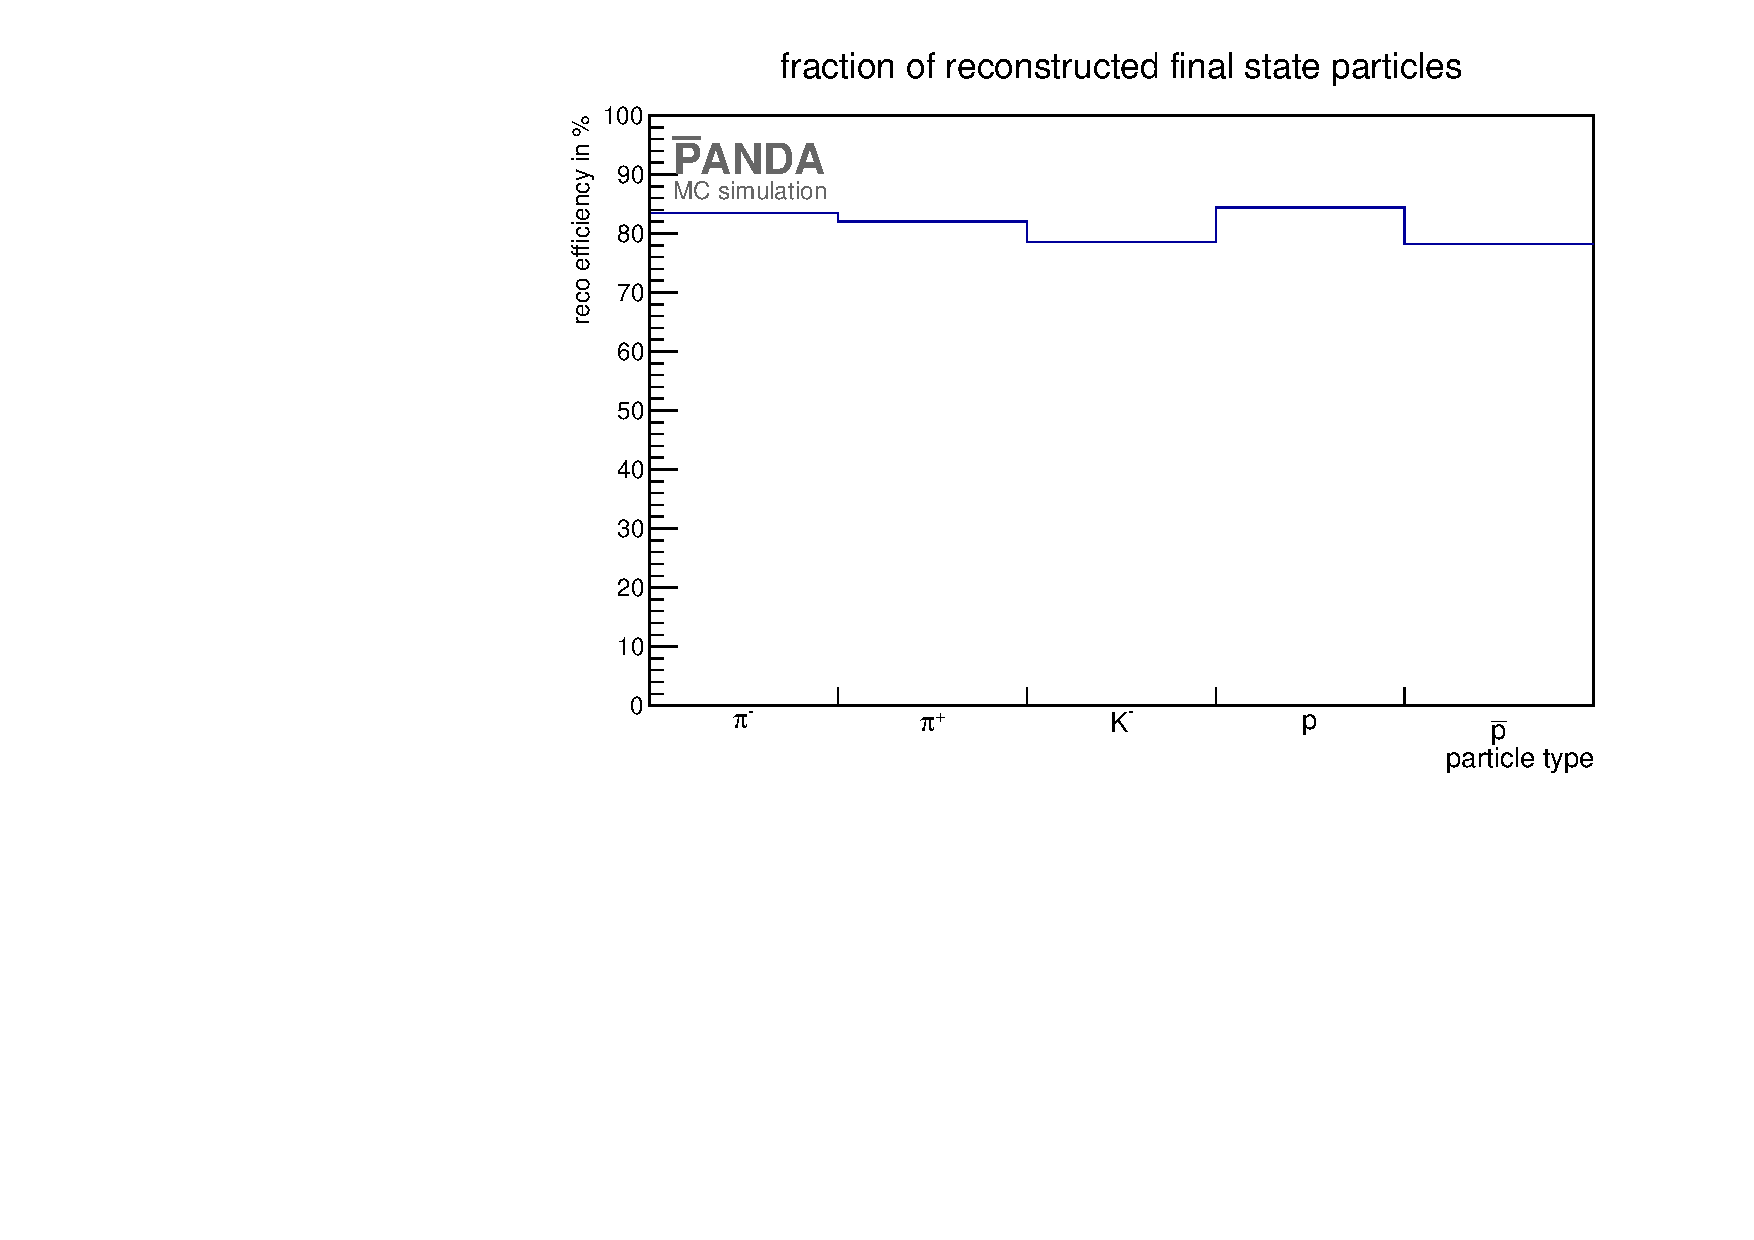
\includegraphics[width=0.8\textwidth]{./plots/finalstate/reco_efficiency.pdf}
		\caption{\propose Reconstruction efficiency for final state particles. The x axis shows the particle type. 
				On the y axis the fraction of reconstructed particles is shown.}
		\label{fig:finalstate_recoeff}
	
	\end{figure}
	

	
\section{Reconstruction of $\Lambda$ and $\bar{\Lambda}$}
	\subsection*{Selection}
		For the reconstruction of \lam hyperons a proton and a \piminus meson are combined and for the reconstruction 
		of \alam a \antiproton and a \piplus are combined.		 
		After combining the daughter particles a mass cut is performed.
		Only those candidates are chosen which have a mass within a window of $0.3$\massunit symmetric to the nominal 
		\lam mass, i.e., a mass within $M= 1.116\pm 0.15$\massunit.
		
		
		A vertex constraint fit with the PndKinVtxFitter is performed on the selected candidate.
		This means that the tracks of the daughter particles are fitted to a common vertex point.  
		The \chisq and probability distribution of the vertex fit for \lam candidates is shown in figure \ref{fig:lambda_chi2}.
		
		\begin{figure}
			\centering
				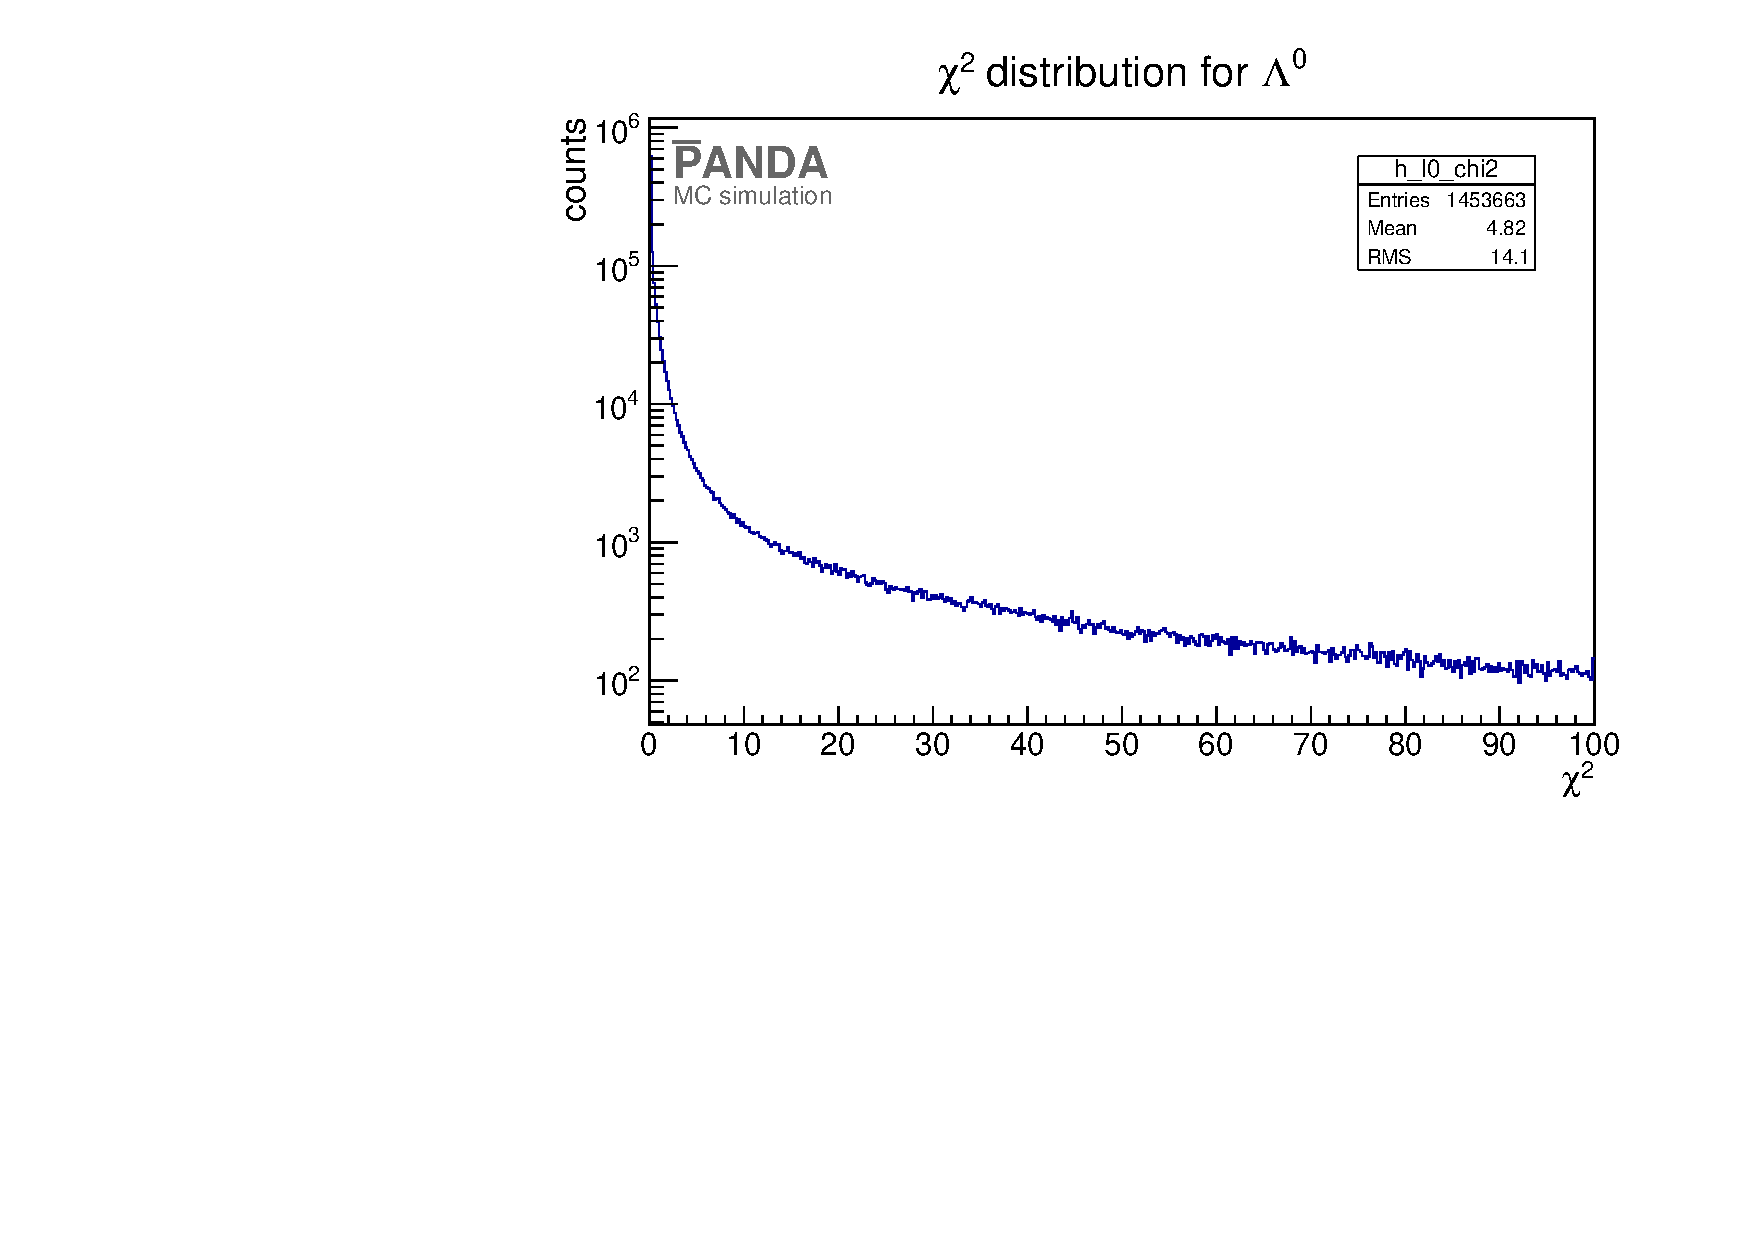
\includegraphics[width=0.50\textwidth]{./plots/lambda0/lambda0_chi2.pdf}
				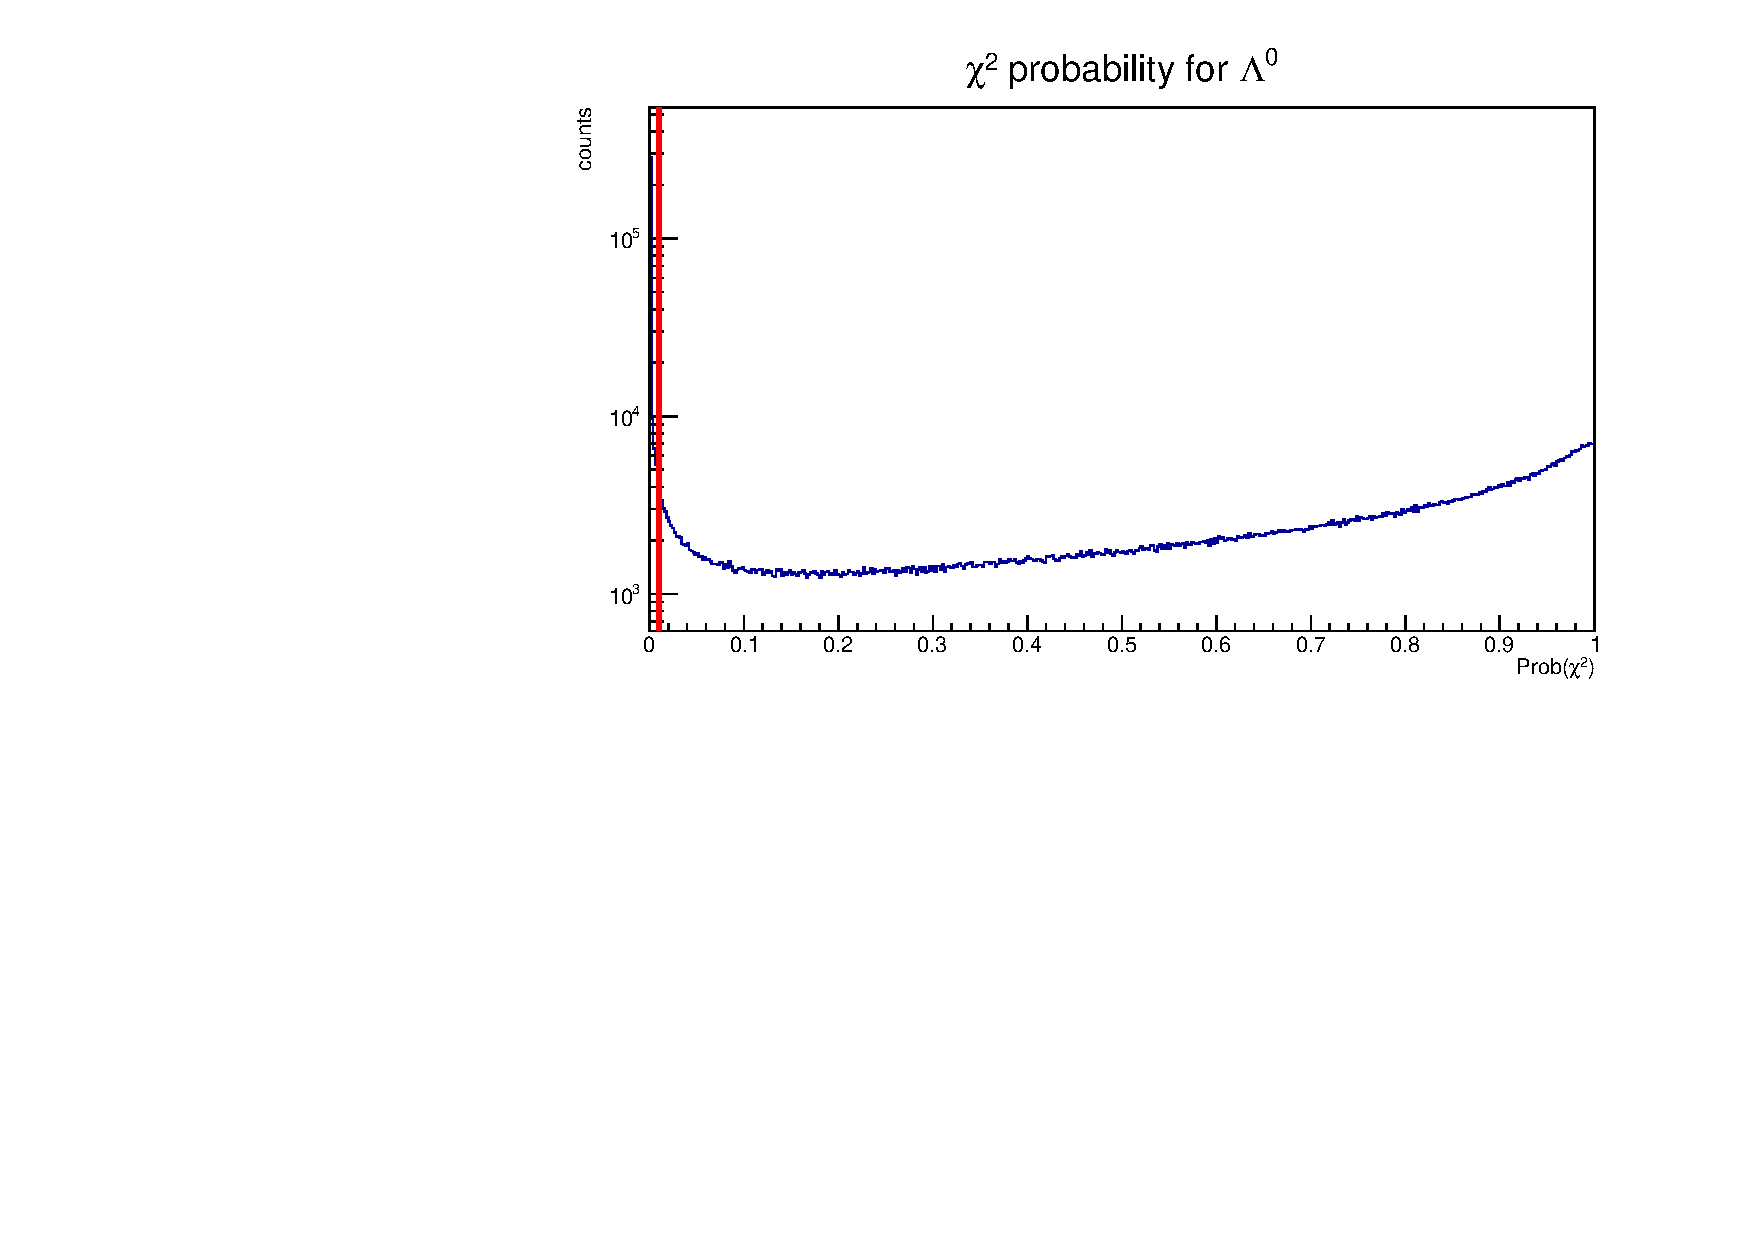
\includegraphics [width=0.50\textwidth]{./plots/lambda0/lambda0_prob.pdf}
			\caption{\propose The upper plot shows the  \chisq distribution and the lower plot shows the probability distribution for the \lam vertex fit.}
			\label{fig:lambda_chi2}
		\end{figure}
		
		In the probability distribution one can see an increasing number of events for probabilities approaching a value of one.
		This feature is not the vertex fit itself, as was shown by tests based on the so-called "poormantrack" algorithm \cite{RalfKliemt}.
		\vspace{11pt}\\
		A mass contraint fit is performed on the fitted candidate.
		For this mass constraint fit the kinematic fitter PndKinFitter is used.
		After using both fitters the selection criterion is set. 
		One select only those particles which have a probability larger than $1\%$ in both fitter.
		A scheme which shows how the events are selected can be found in figure \ref{fig:lambda_scheme}. 
		
		\begin{figure}
			\centering
				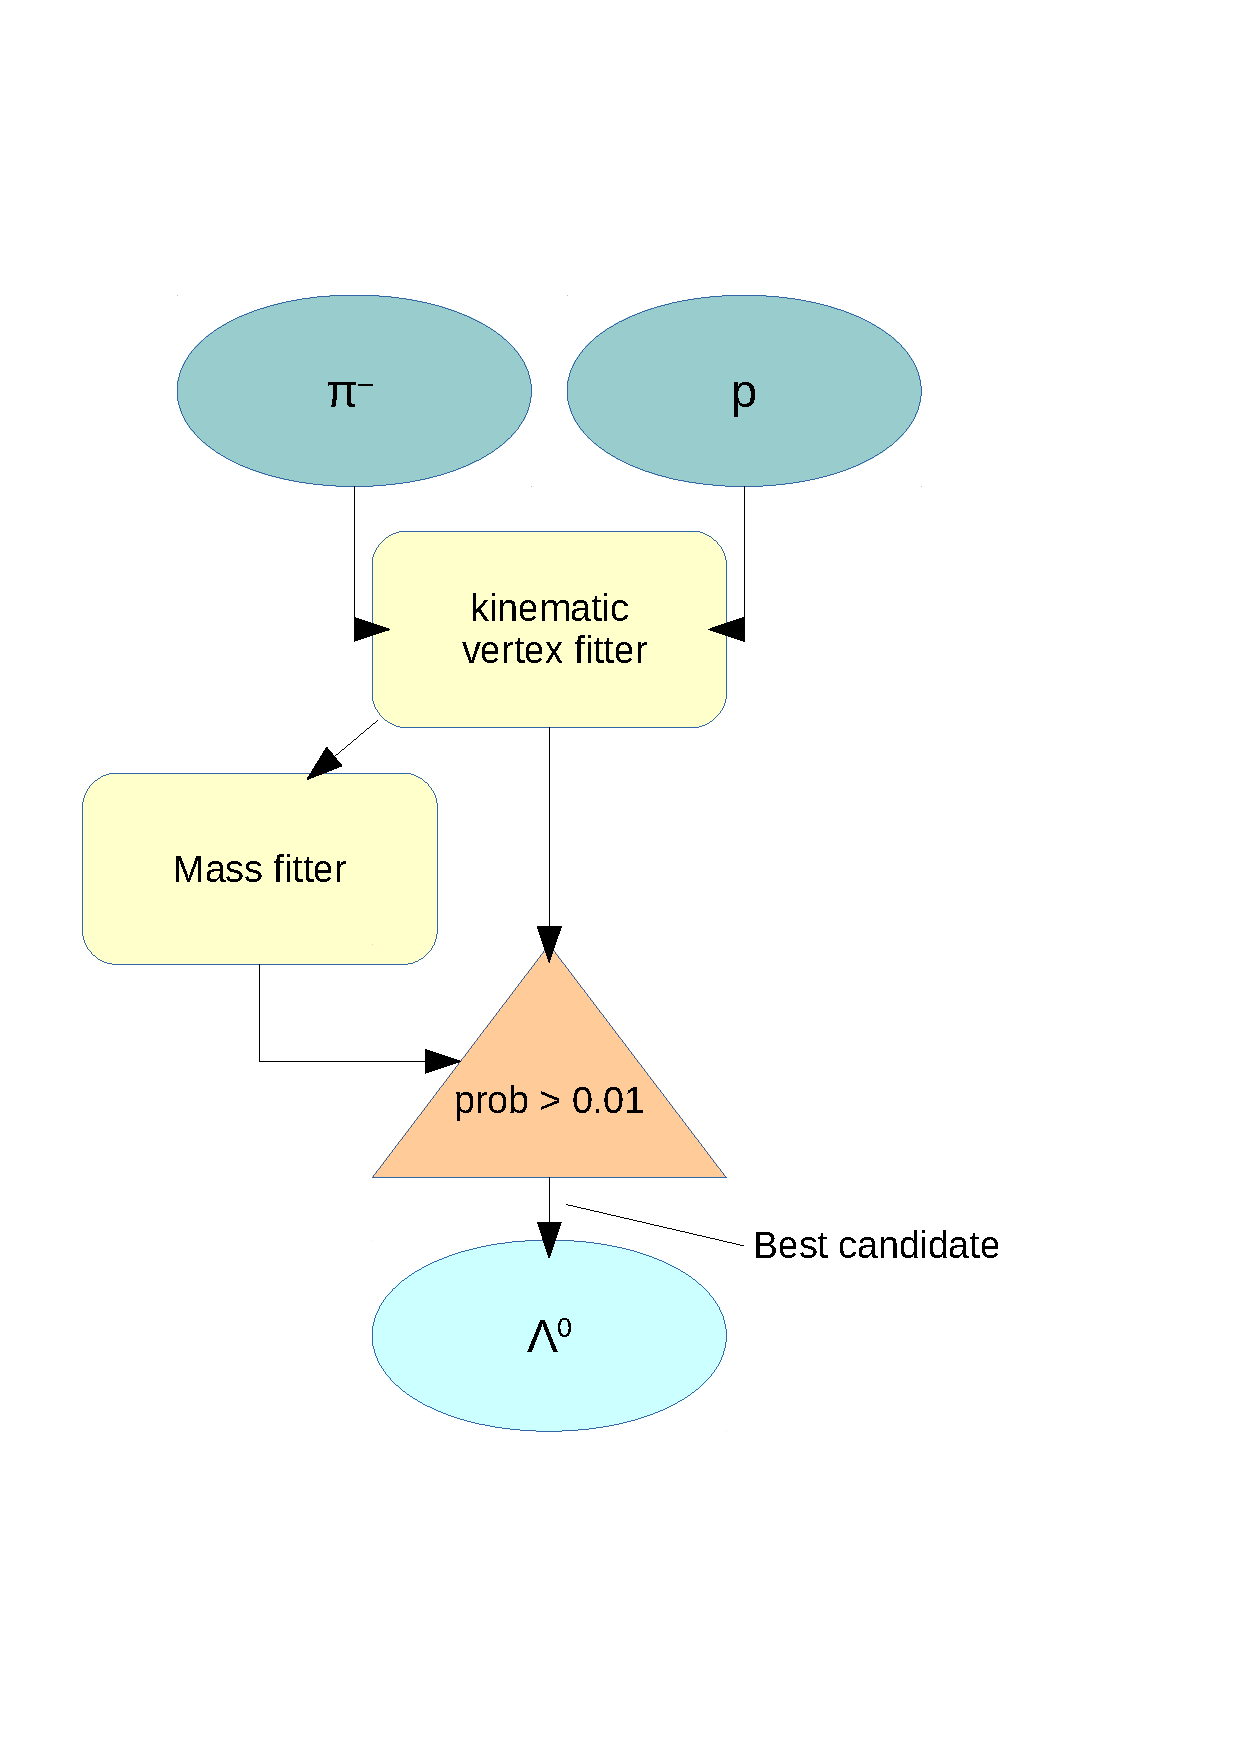
\includegraphics[width=0.45\textwidth]{./plots/combineLambda0.pdf}
			\caption{\propose Scheme for \lam reconstruction}
			\label{fig:lambda_scheme}
		\end{figure}
		
		If there is more than one candidate left after these cuts, the candidate with the lowest \chisq is chosen.
		
		
	\subsection*{Results}
		In this paragraph the \lam and \alam sample obtained with the chosen selection criteria is presented.
		The mass distributions correspondingt to the different cuts are shown in figure \ref{fig:lambda0_massdiffcuts} 
		and figure \ref{fig:antilambda0_massdiffcuts} for \lam and \alam, respectively.
	
		\begin{figure}
			\centering
				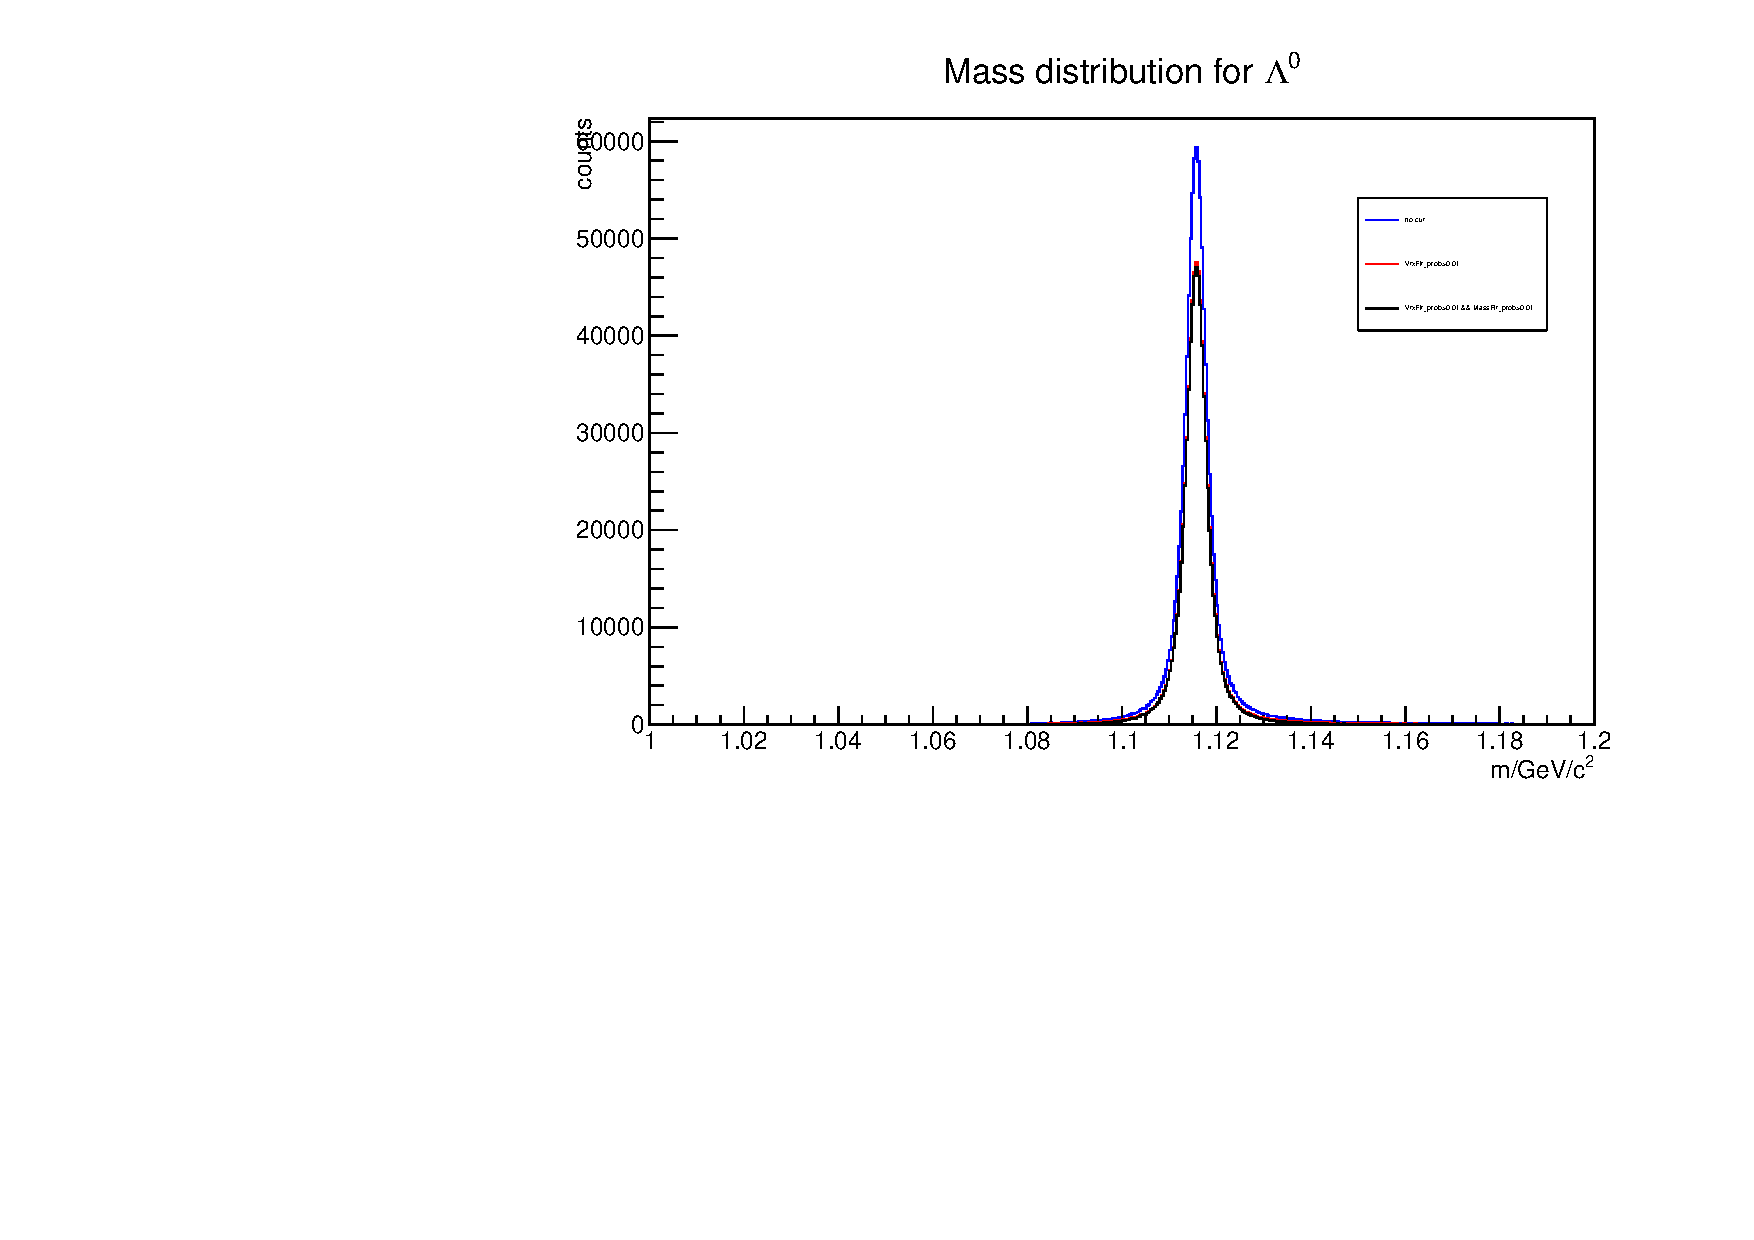
\includegraphics[width=1.1\textwidth]{./plots/lambda0/lambda0_m_diffcuts.pdf}
			\caption{\propose Mass distribution of \lam after the mass cut (blue), after the vertex fit cut (red) and after all cuts (black).}
			\label{fig:lambda0_massdiffcuts}
		\end{figure}
			
		\begin{figure}
			\centering
				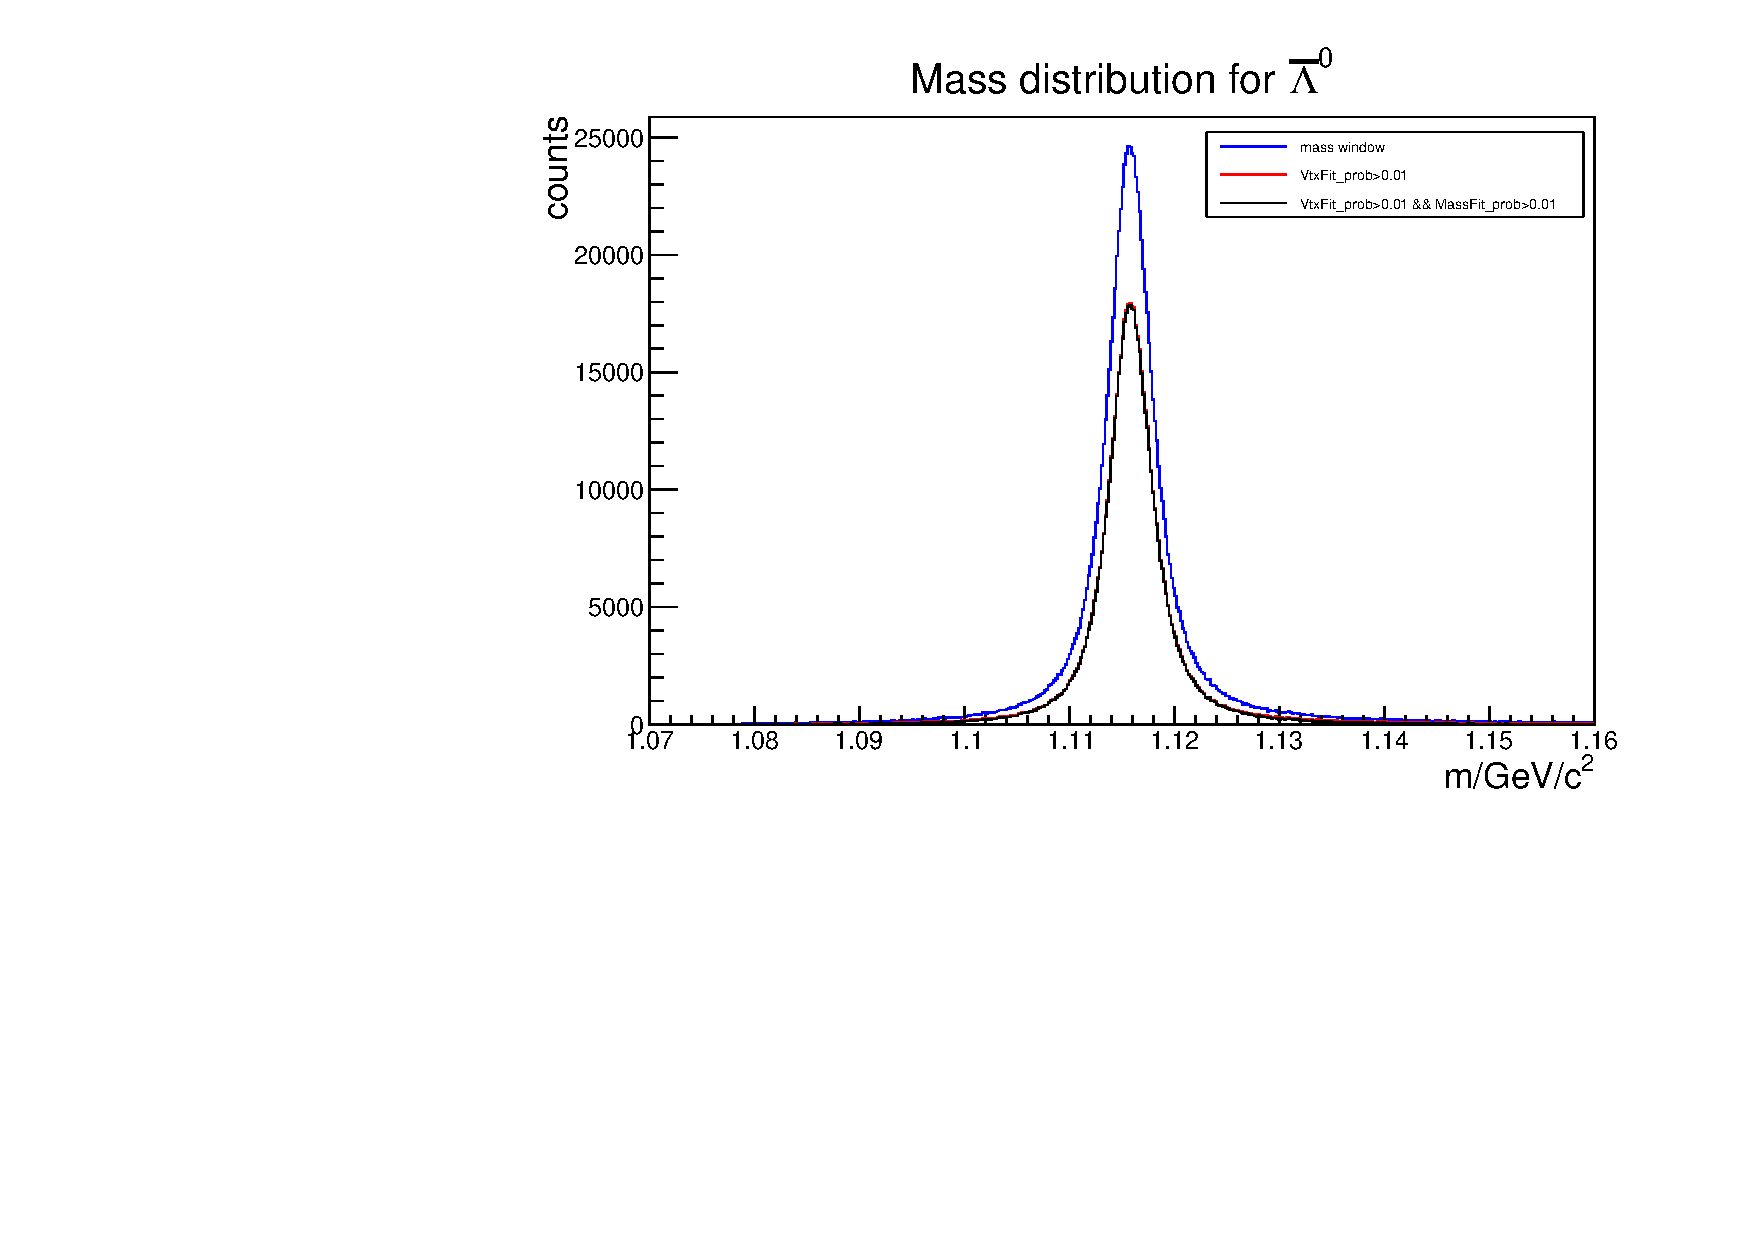
\includegraphics[width=1.1\textwidth]{./plots/antilambda0/antiLambda0_m_diffcuts.pdf}
			\caption{\propose Mass distribution of \alam after the mass cut (blue), after the vertex fit cut (red) and after all cuts (black).}
			\label{fig:antilambda0_massdiffcuts}
		\end{figure}
		
		The reconstructed mass can be determined by performing a double Gaussian fit on the mass distribution obtained after all cuts.
		The mass distribution and the double Gaussian fit are shown for \lam candidates in figure \ref{fig:lambda0_massfit}.
		
		\begin{figure}
			\centering
				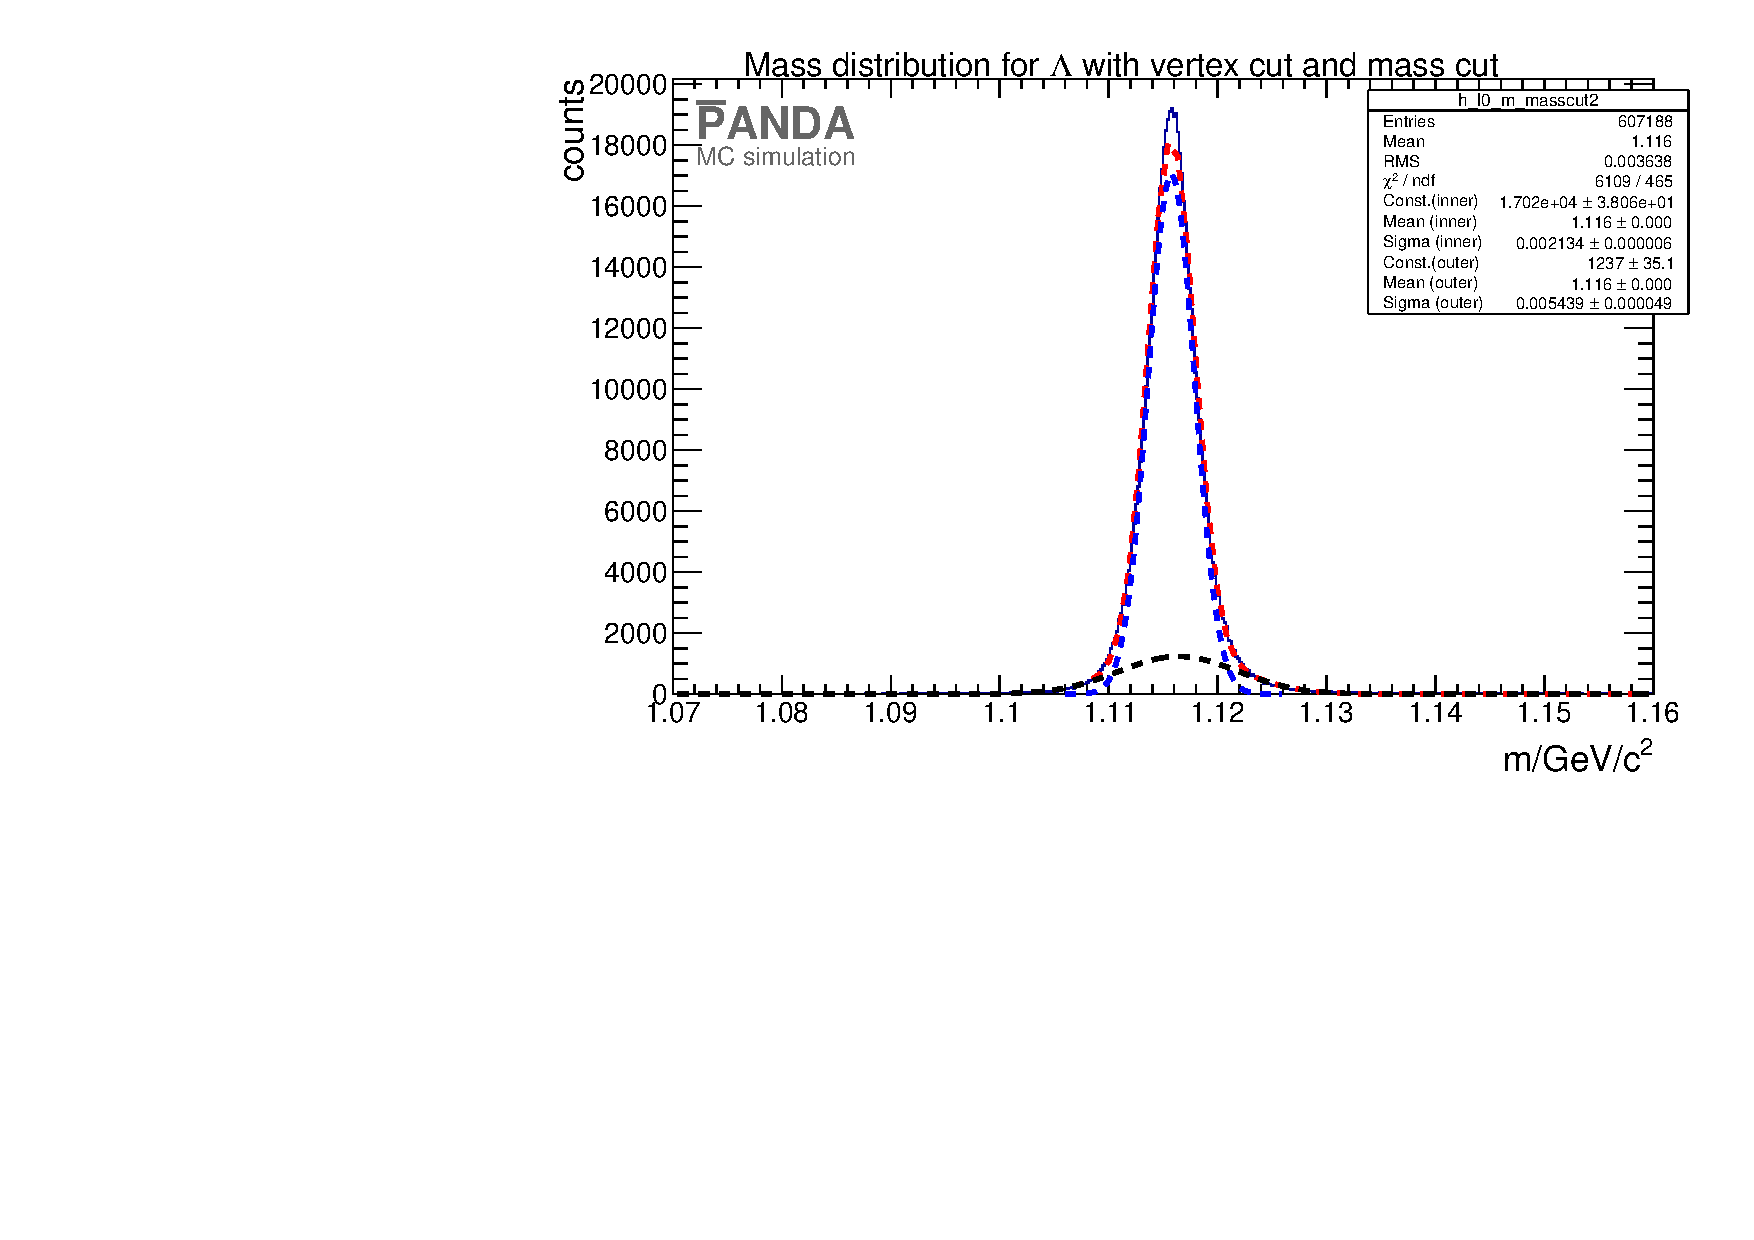
\includegraphics[width=0.8\textwidth]{./plots/lambda0/lambda0_m_masscut2.pdf}
			\caption{\propose Mass distribution (blue histogram) for \lam fitted with a double Gaussian fit (red dashed line).}
			\label{fig:lambda0_massfit}
		\end{figure}
		
		The peak position of the Gaussian fit is taken as the value of the reconstructed mass.
		The reconstructed masses are $\mt{m}_{\Lambda^0} = \left(1.1158 \pm 0.0022\right)$\massunit and 
		$\mt{m}_{\bar{\Lambda}^0} = \left(1.1159 \pm 0.0022\right)$\massunit for \lam and \alam, respectively. 
		Figure \ref{fig:lambda0_pt_vs_pz} shows the transverse momentum versus the longitudinal momentum.
				
		\begin{figure}
			
			\subfigure[]{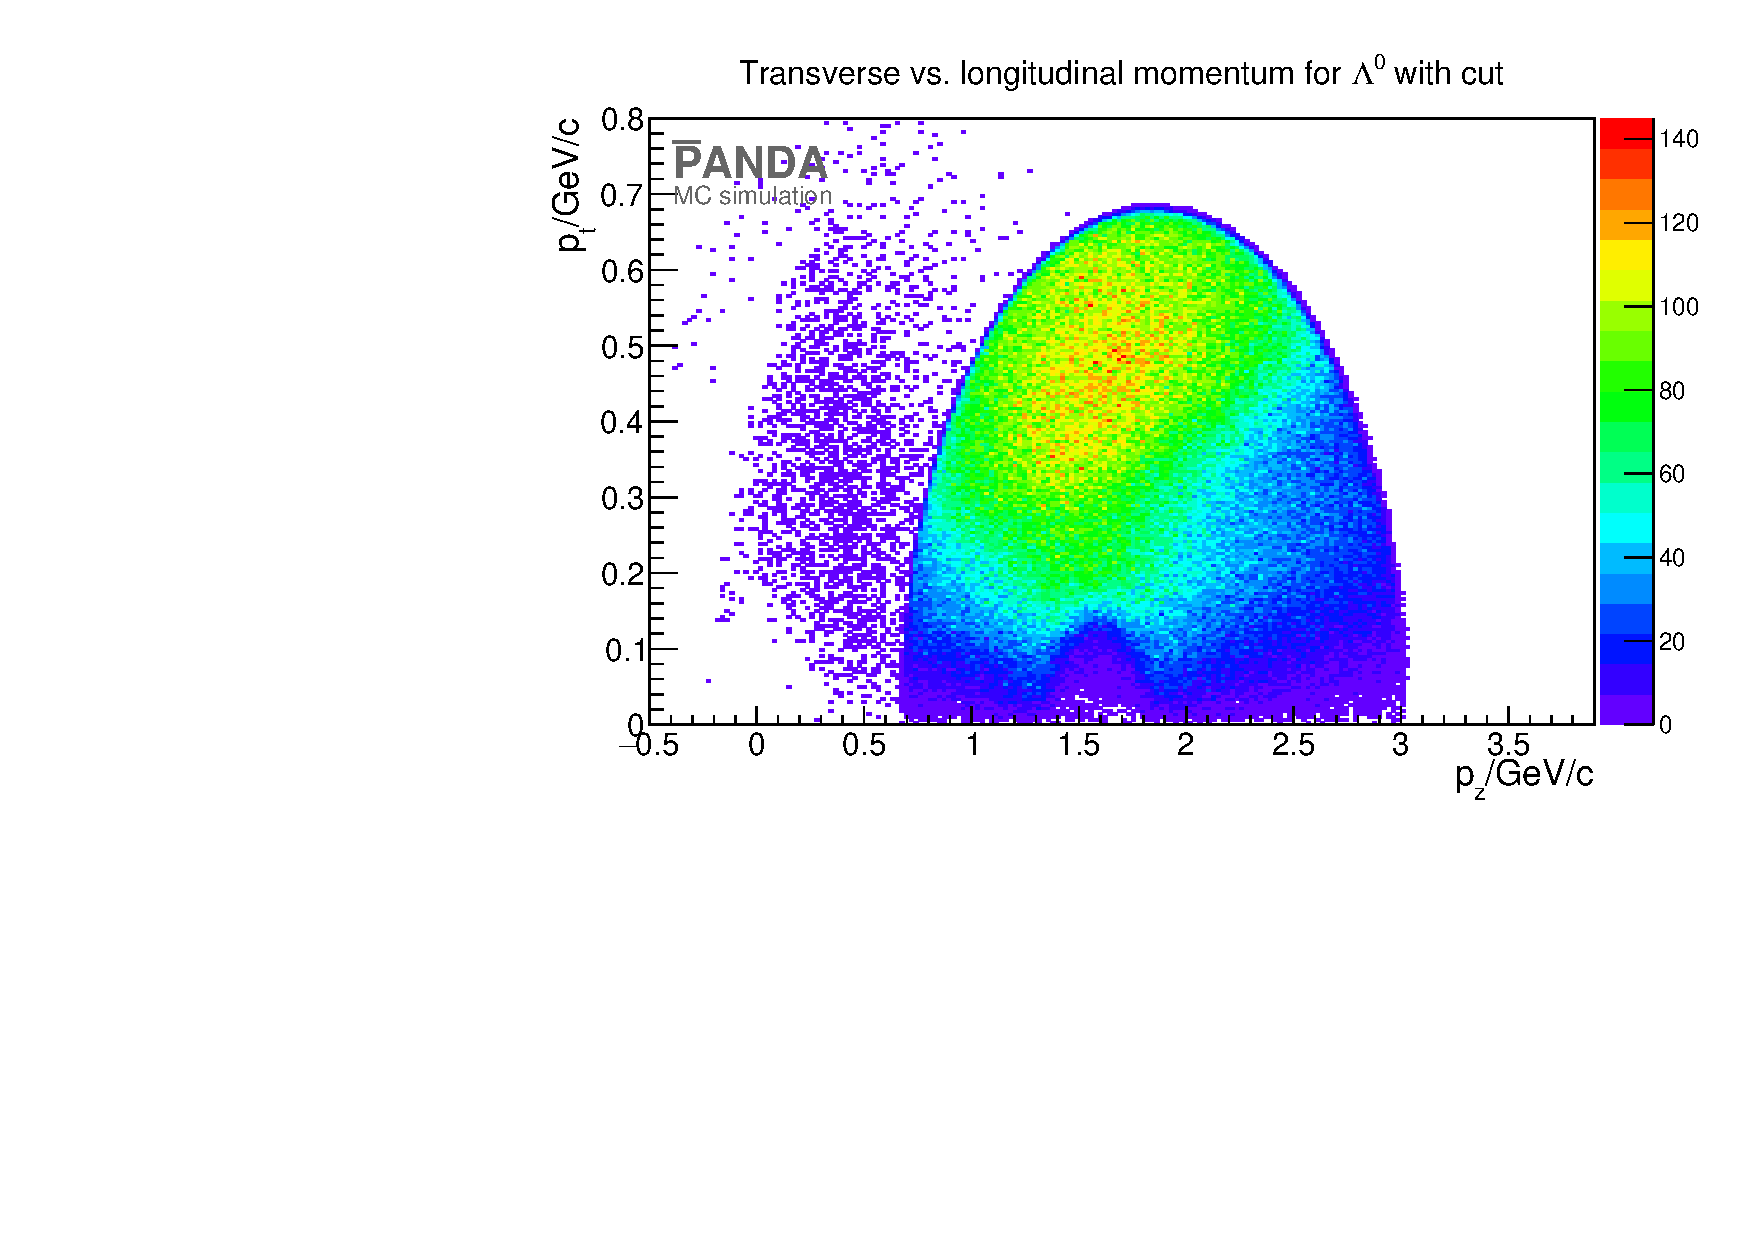
\includegraphics[width=0.49\textwidth]{./plots/lambda0/lambda0_pt_vs_pz_cut.pdf}}
			\subfigure[]{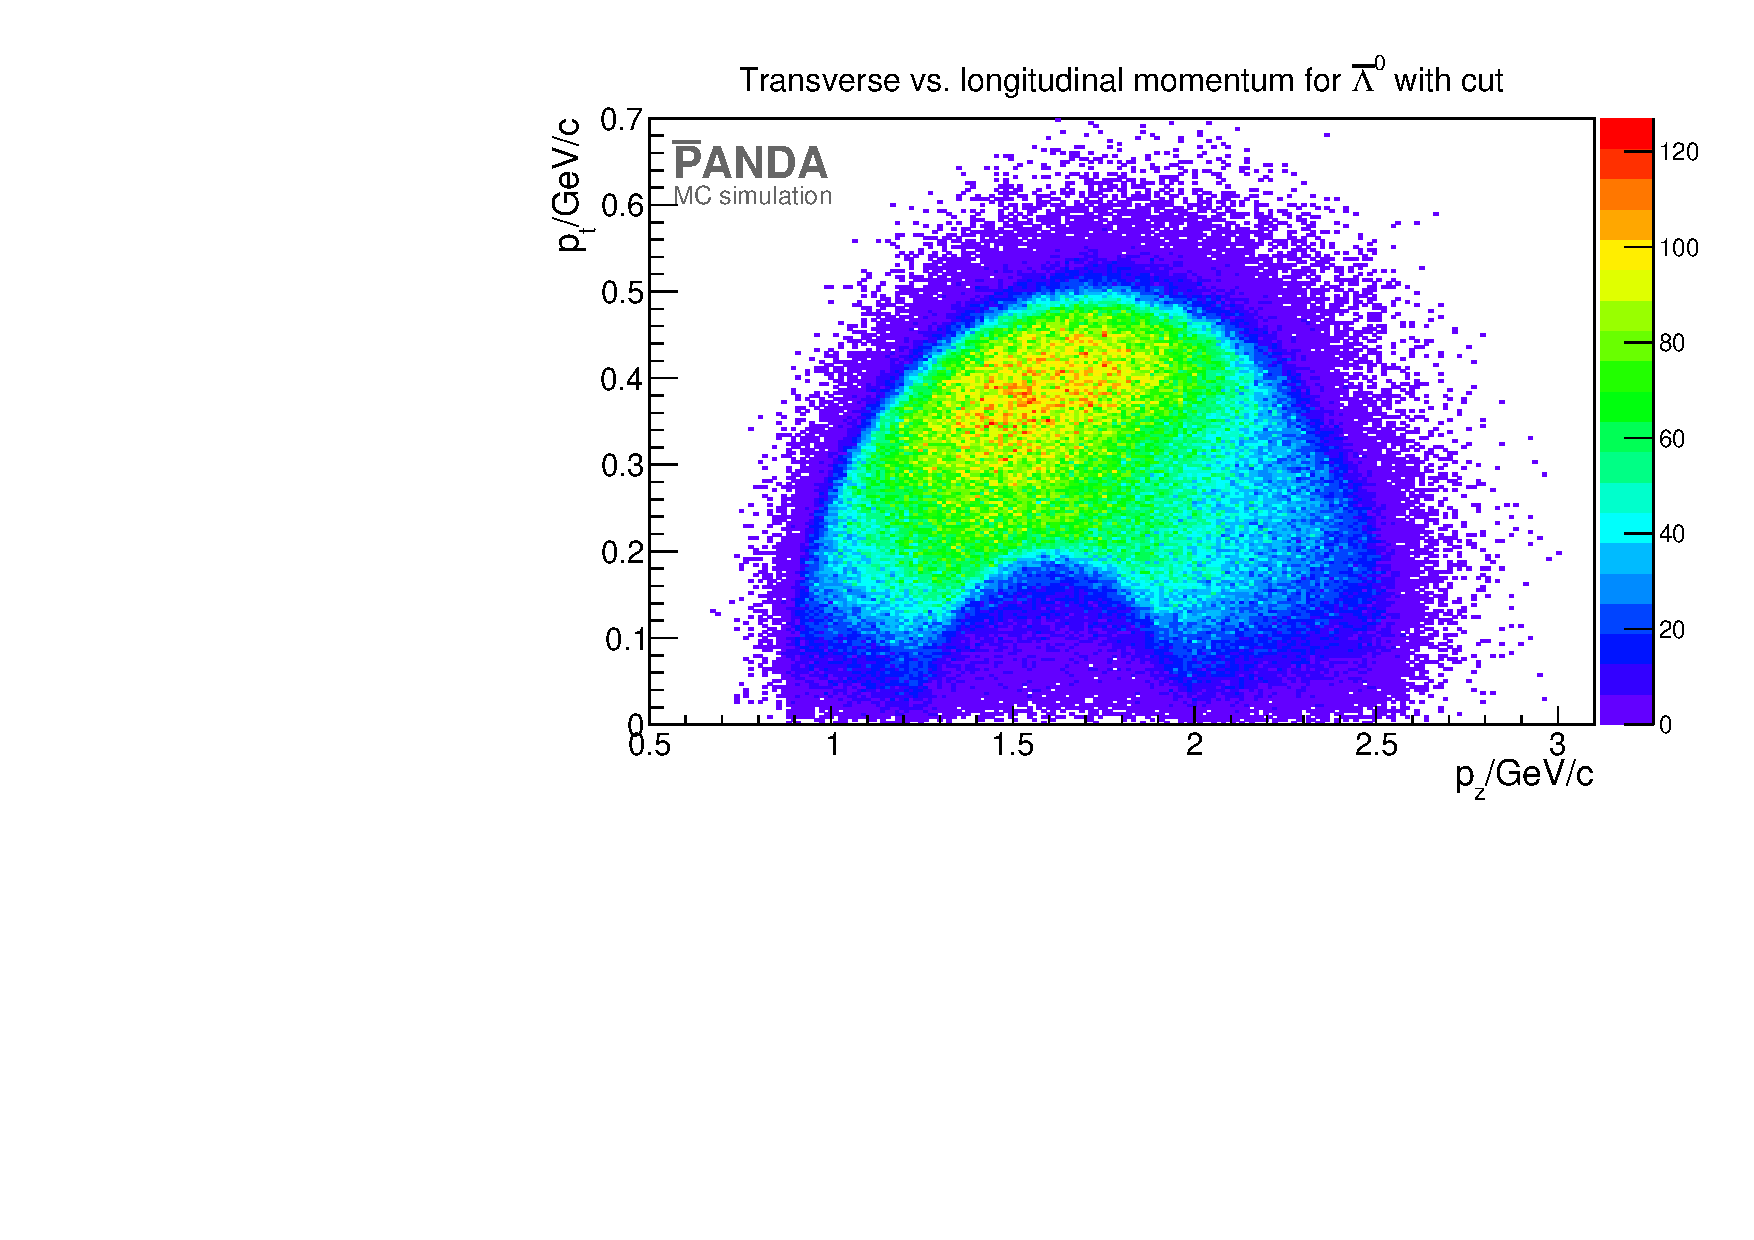
\includegraphics[width=0.49\textwidth]{./plots/antilambda0/antiLambda0_pt_vs_pz_cut.pdf}}
			\caption{\propose Figure a): transverse versus longitudinal momentum for \lam. Figure b):transverse versus longitudinal momentum for \alam.}
			\label{fig:lambda0_pt_vs_pz}
		
		\end{figure}
		After all cuts the reconstruction efficiency is $50.33\%$ for \lam and $41.46\%$ for \alam.
		The difference in the reconstruction efficiencies for \lam and \alam is caused by the different decay lengths of their mother particles.
		\lam is emitted by the \excitedcascade which has a very short decay length while the decay length of \anticascade is 
		c$\tau = 4.91 \unit{cm}$ \cite{PDG}.
		The decay length of \lam and \alam is $\textnormal{c}\tau = 7.98 \unit{cm}$, so that the final state particles of \alam are produced more downstream 
		than the final state particles of \lam.
		This can be also seen in figure \ref{fig:lambda0_antilambda0_decay_vtx}.
		The finale state particles of \alam are produced at the edge of the MVD detector so that the reconstruction efficiency for these particles is reduced.
		
		\begin{figure}
		
			\centering
			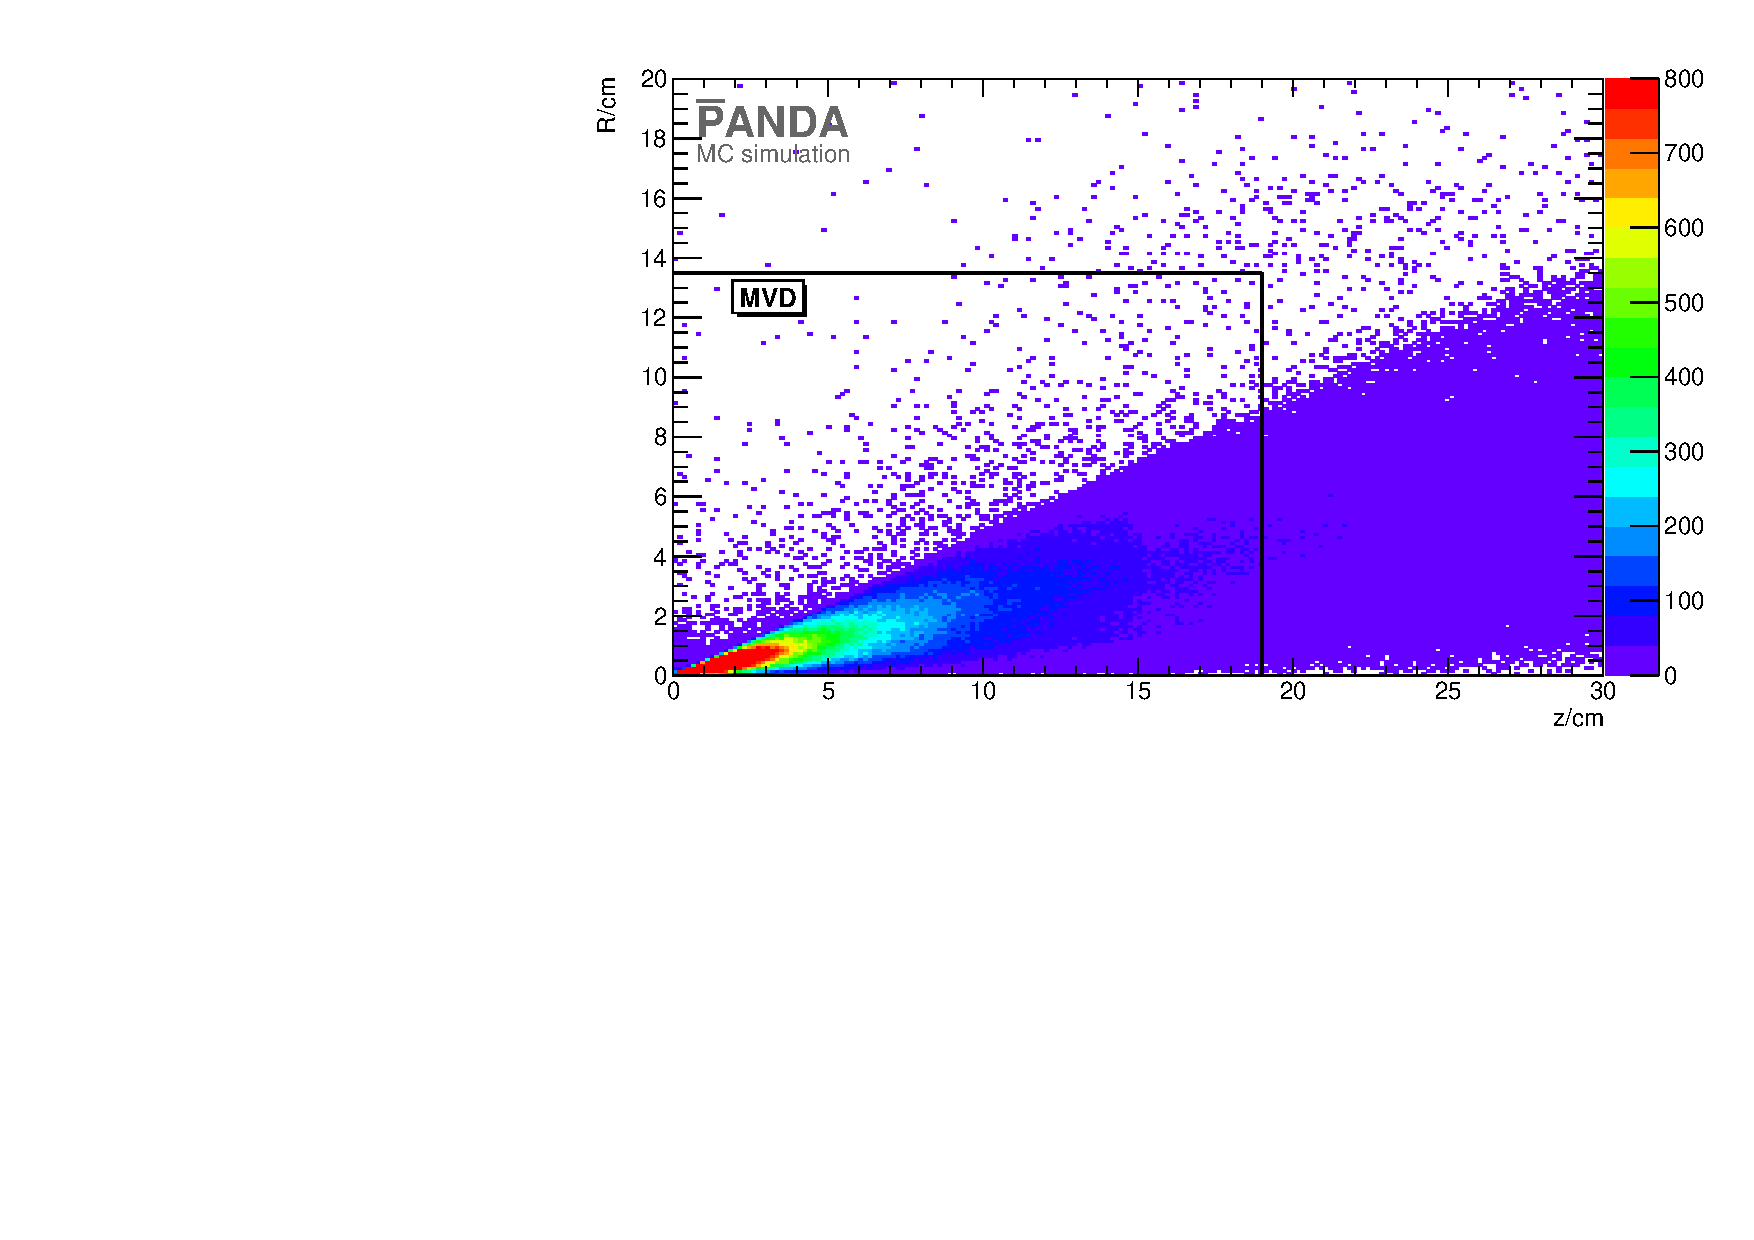
\includegraphics[width=1.\textwidth]{./plots/lambda0/lambda0_decay_vtx.pdf}
			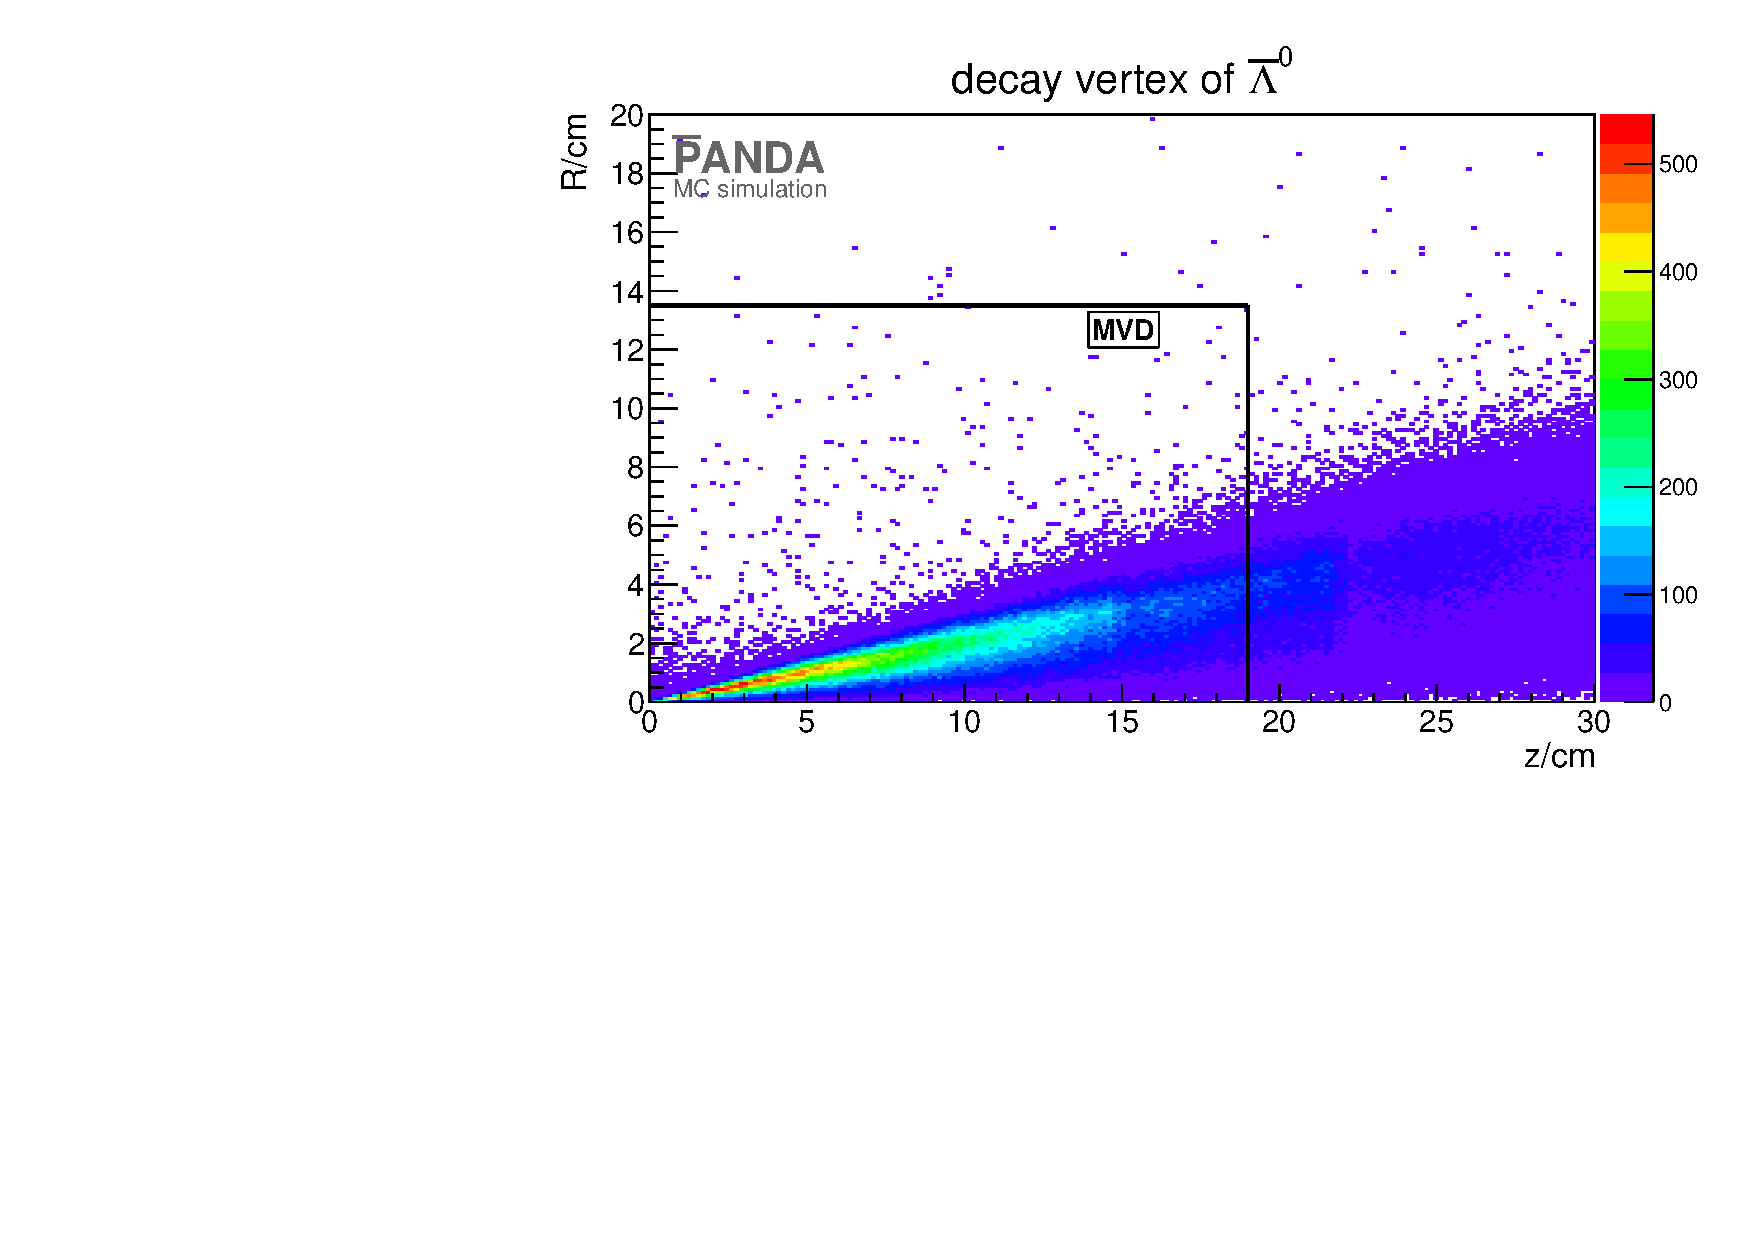
\includegraphics[width=1.\textwidth]{./plots/antilambda0/antiLambda0_decay_vtx.pdf}
			\caption{\propose Decay vertex position of \lam (upper plot) and \alam (lower plot). 
					In both plots the x axis shows the z coordinate (along the beam axis) of the 
					decay vertex while the y axis shows its radial coordinate (the origin of the coordinate system s defined by the primary vertex).
					The black horizontal and vertical lines mark the radial and longitudinal extension of the MVD.}
			\label{fig:lambda0_antilambda0_decay_vtx}
		
		\end{figure}
		
		
		
		
	
\section{Reconstruction of \cascade and \anticascade}
	\subsection*{Selection}
		The reconstruction of \cascade and \anticascade follows a similar scheme like the reconstruction of \lam and \alam.
		For \anticascade are \alam and \piplusone recombined and for \cascade in the charge conjugate. channel \lam and \piminusone.
		Now it is distinguished between the to \piplus (\piminus) particle and use only those particles which have not already been combined.
		After combining the daughter particles a mass window cut is performed with a width of $0.3$\massunit around 
		the \cascade mass $m_{\Xi} = 1.32171$ \massunit \cite{PDG}.
		 
		The fitting scheme is the same as for \lam and \alam and is shown in figure \ref{fig:anticascade_scheme} 
		After the mass window cut the daughter particles are fitted to a common vertex with the PndKinVtxFitter.
		And again these information is used to perform the mass constraint fit. 
		
		\begin{figure}
			\centering
				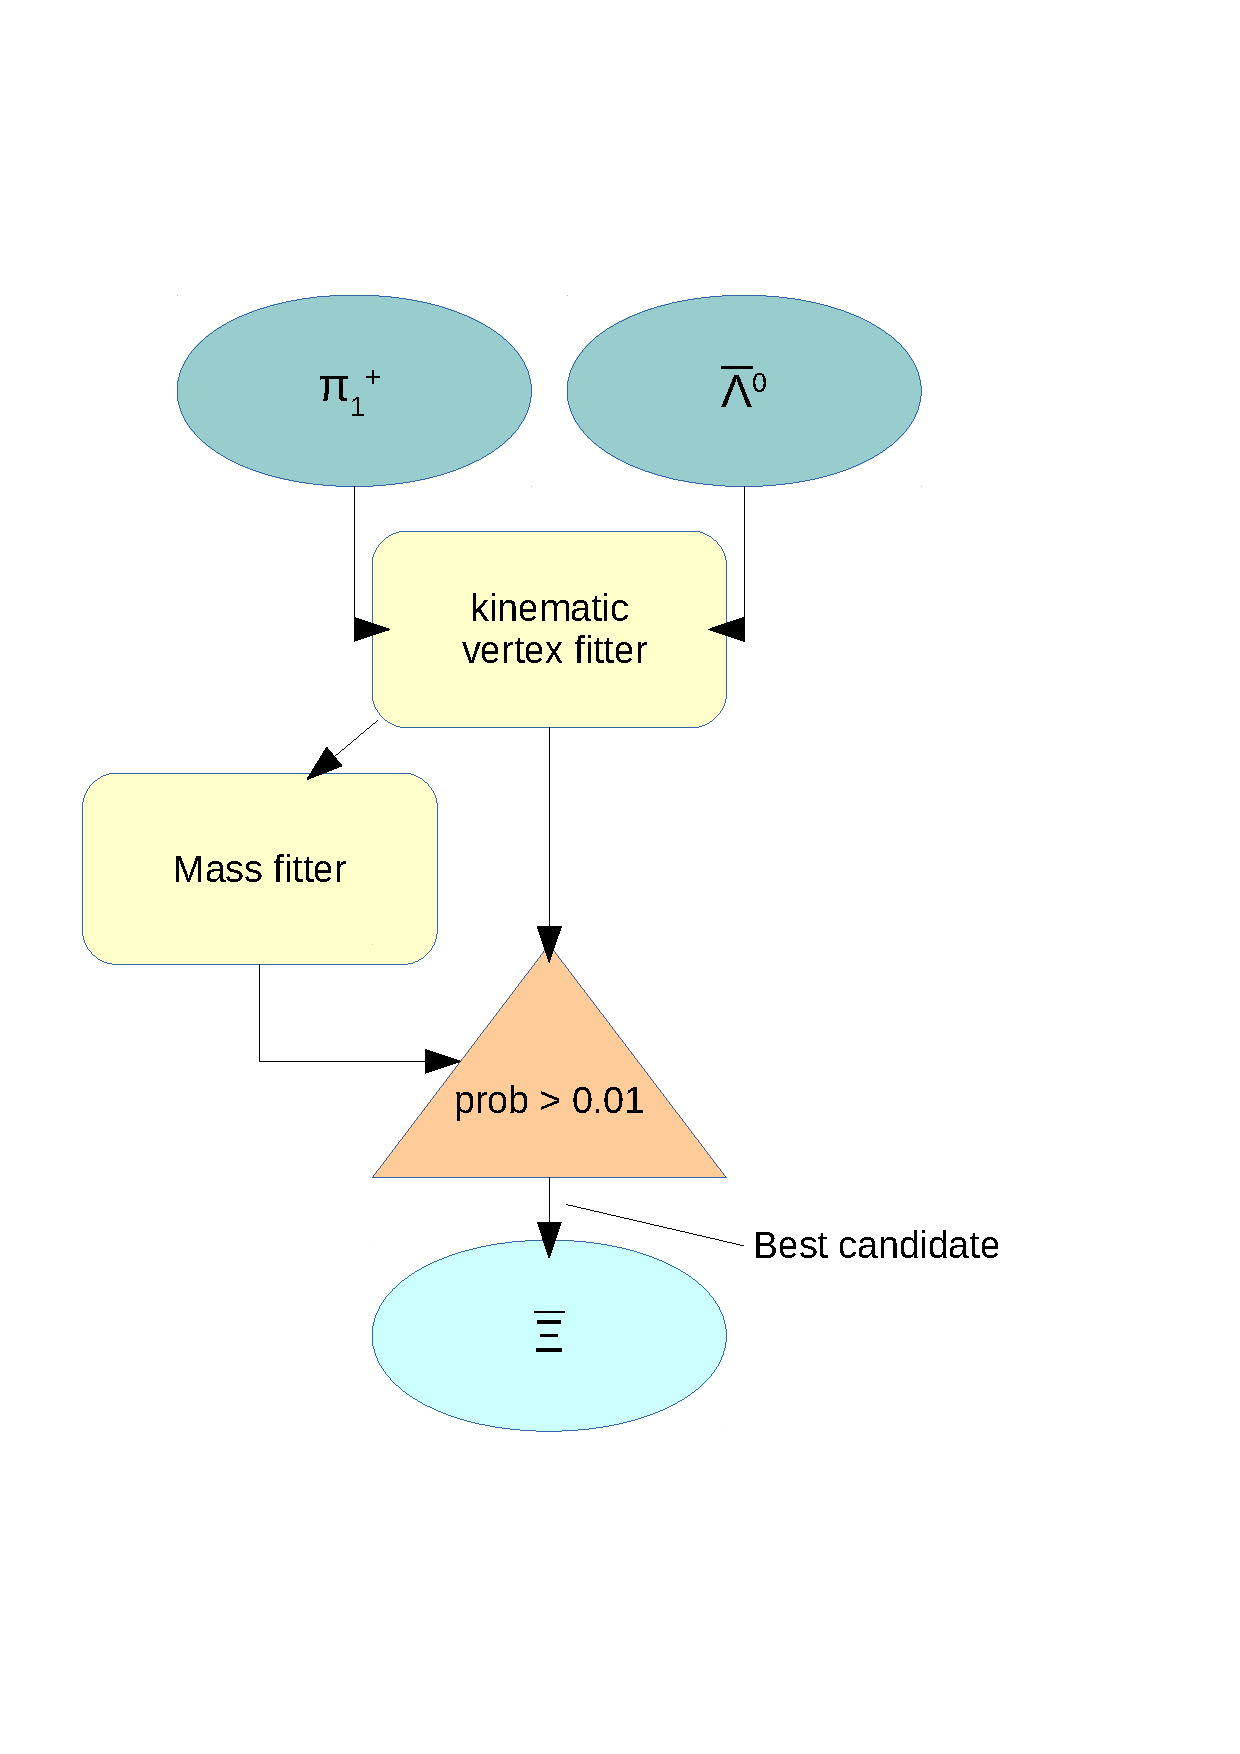
\includegraphics[width=0.50\textwidth]{./plots/combineAntiCascade.pdf}
			\caption{\propose Scheme for \anticascade reconstruction}
			\label{fig:anticascade_scheme}
		\end{figure}
		
		Only those particles are selected which have a \chisq probability of more than $1\,\%$ in both fitter. 
		Figure \ref{fig:XiPlus_prob} shows exemplarily the cut on the vertex fit probability.
		
		\begin{figure}
			\centering
				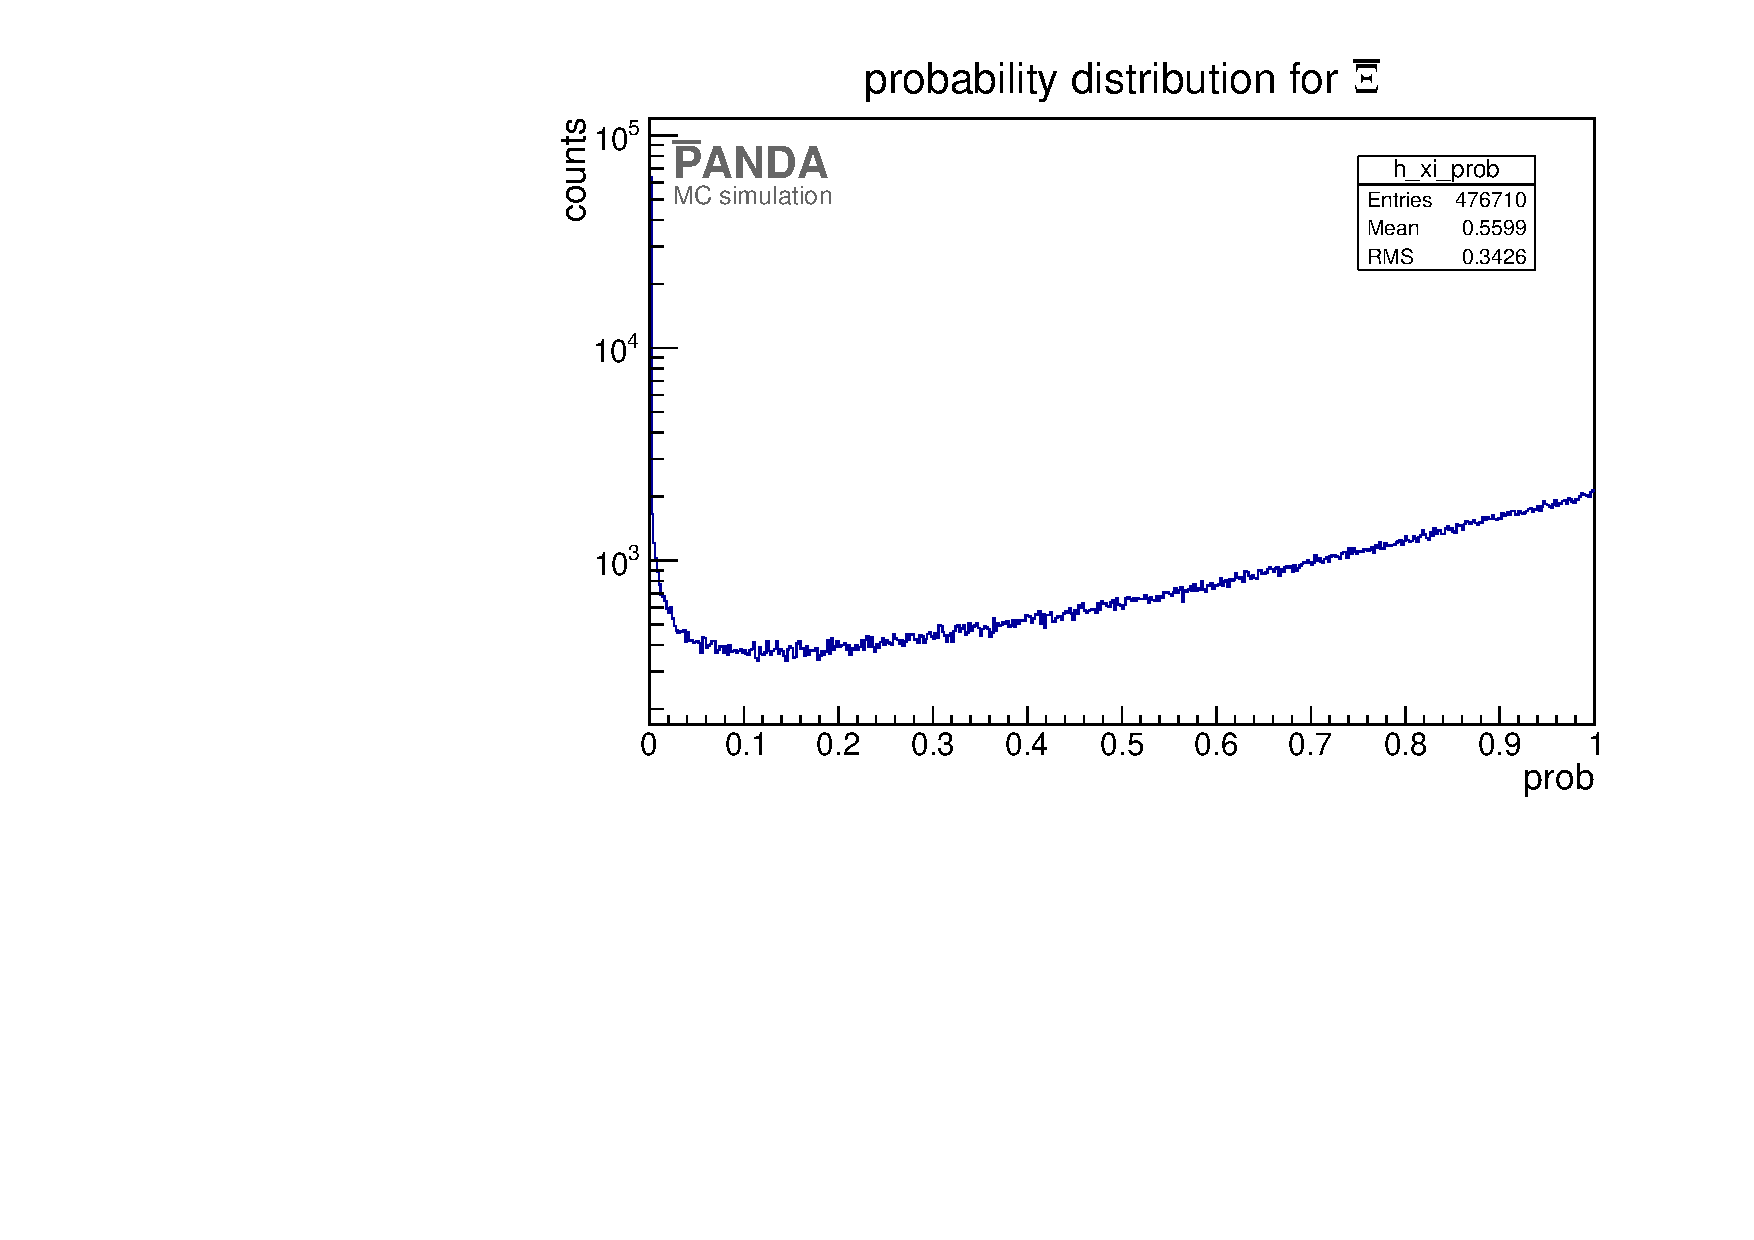
\includegraphics[width=0.50\textwidth]{./plots/Xi/XiPlus_prob.pdf}
			\caption{\propose \chisq probability for \anticascade reconstruction}
			\label{fig:XiPlus_prob}
		\end{figure}
			
		If there is more than one candidate left after all cuts, the best candidate is chosen.
		
		
	\subsection*{Results}
		The vertex resolution after all cuts is shown in table \ref{tab:XiPlus_vtxres}. 
		
		\begin{table}
			\centering
			\caption{\propose Vertex resolution for \anticascade and \cascade (charge conjugate. channel)}
			\label{tab:XiPlus_vtxres}
			\begin{tabular}{ccc}
				\hline
				position & \anticascade & \cascade(from charge conjugate.) \\\hline
				\hline
				x/cm & $0.052$ & $0.056$\\
				y/cm & $0.052$ & $0.052$\\
				z/cm & $0.192$ & $0.2$\\
				\hline
				    
			\end{tabular}
		\end{table}
		
		It is determined by calculating the full width at half maximum (FWHM) of the distribution.
		The advantage of using this method for calculating the vertex resolution is that the FWHM is independent of distribution shape.
		Figure \ref{fig:xi_vtxres_x} and Figure \ref{fig:xi_vtxres_yz} show the vertex resolution. 
		
		\begin{figure}
			\centering
			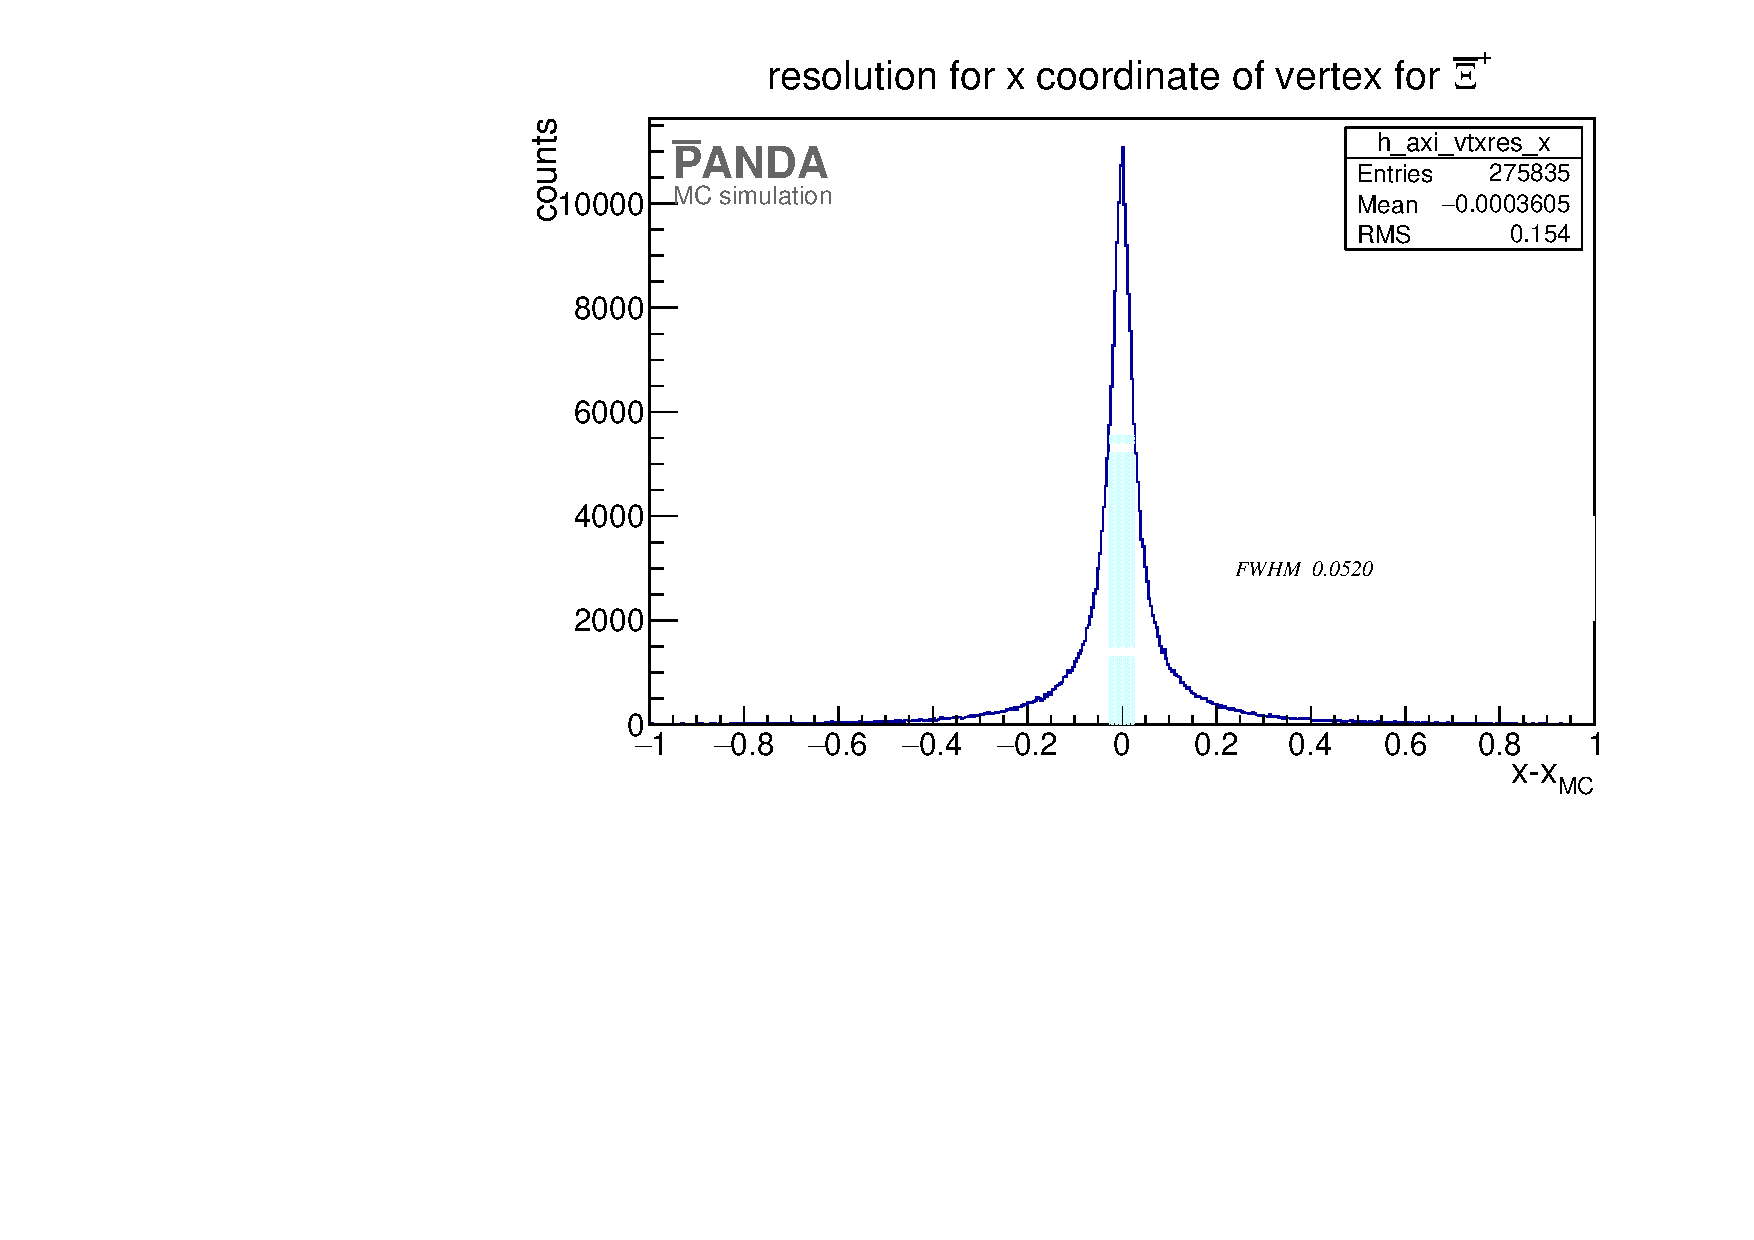
\includegraphics[width=0.8\textwidth]{./plots/Xi/XiPlus_vtxres_x.pdf}
			\caption{\propose Vertex resolution of x position for \anticascade}
			\label{fig:xi_vtxres_x}
			
		\end{figure}
		
		\begin{figure}
			\subfigure[Vertex resolution for y coordinate]{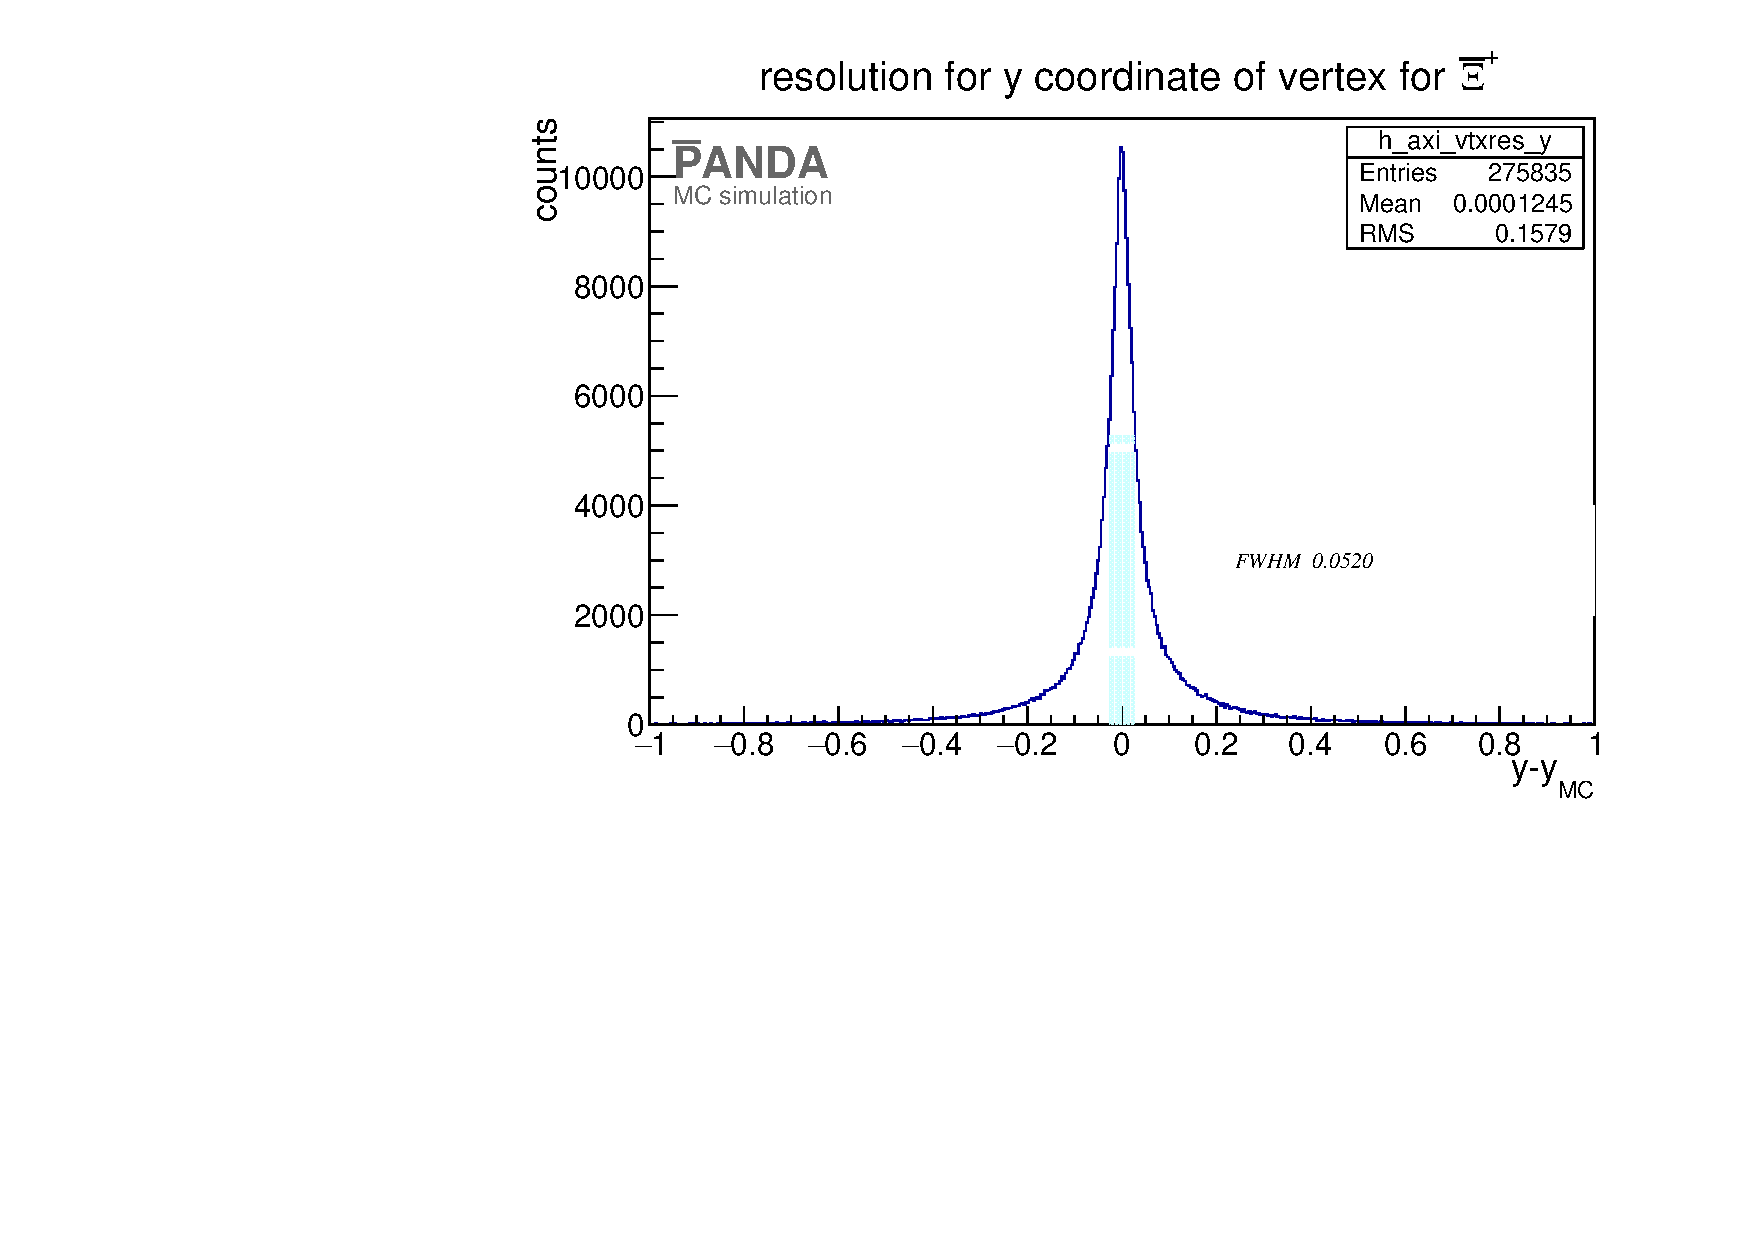
\includegraphics[width=0.49\textwidth]{./plots/Xi/XiPlus_vtxres_y.pdf}}
			\subfigure[Vertex resolution for z coordinate]{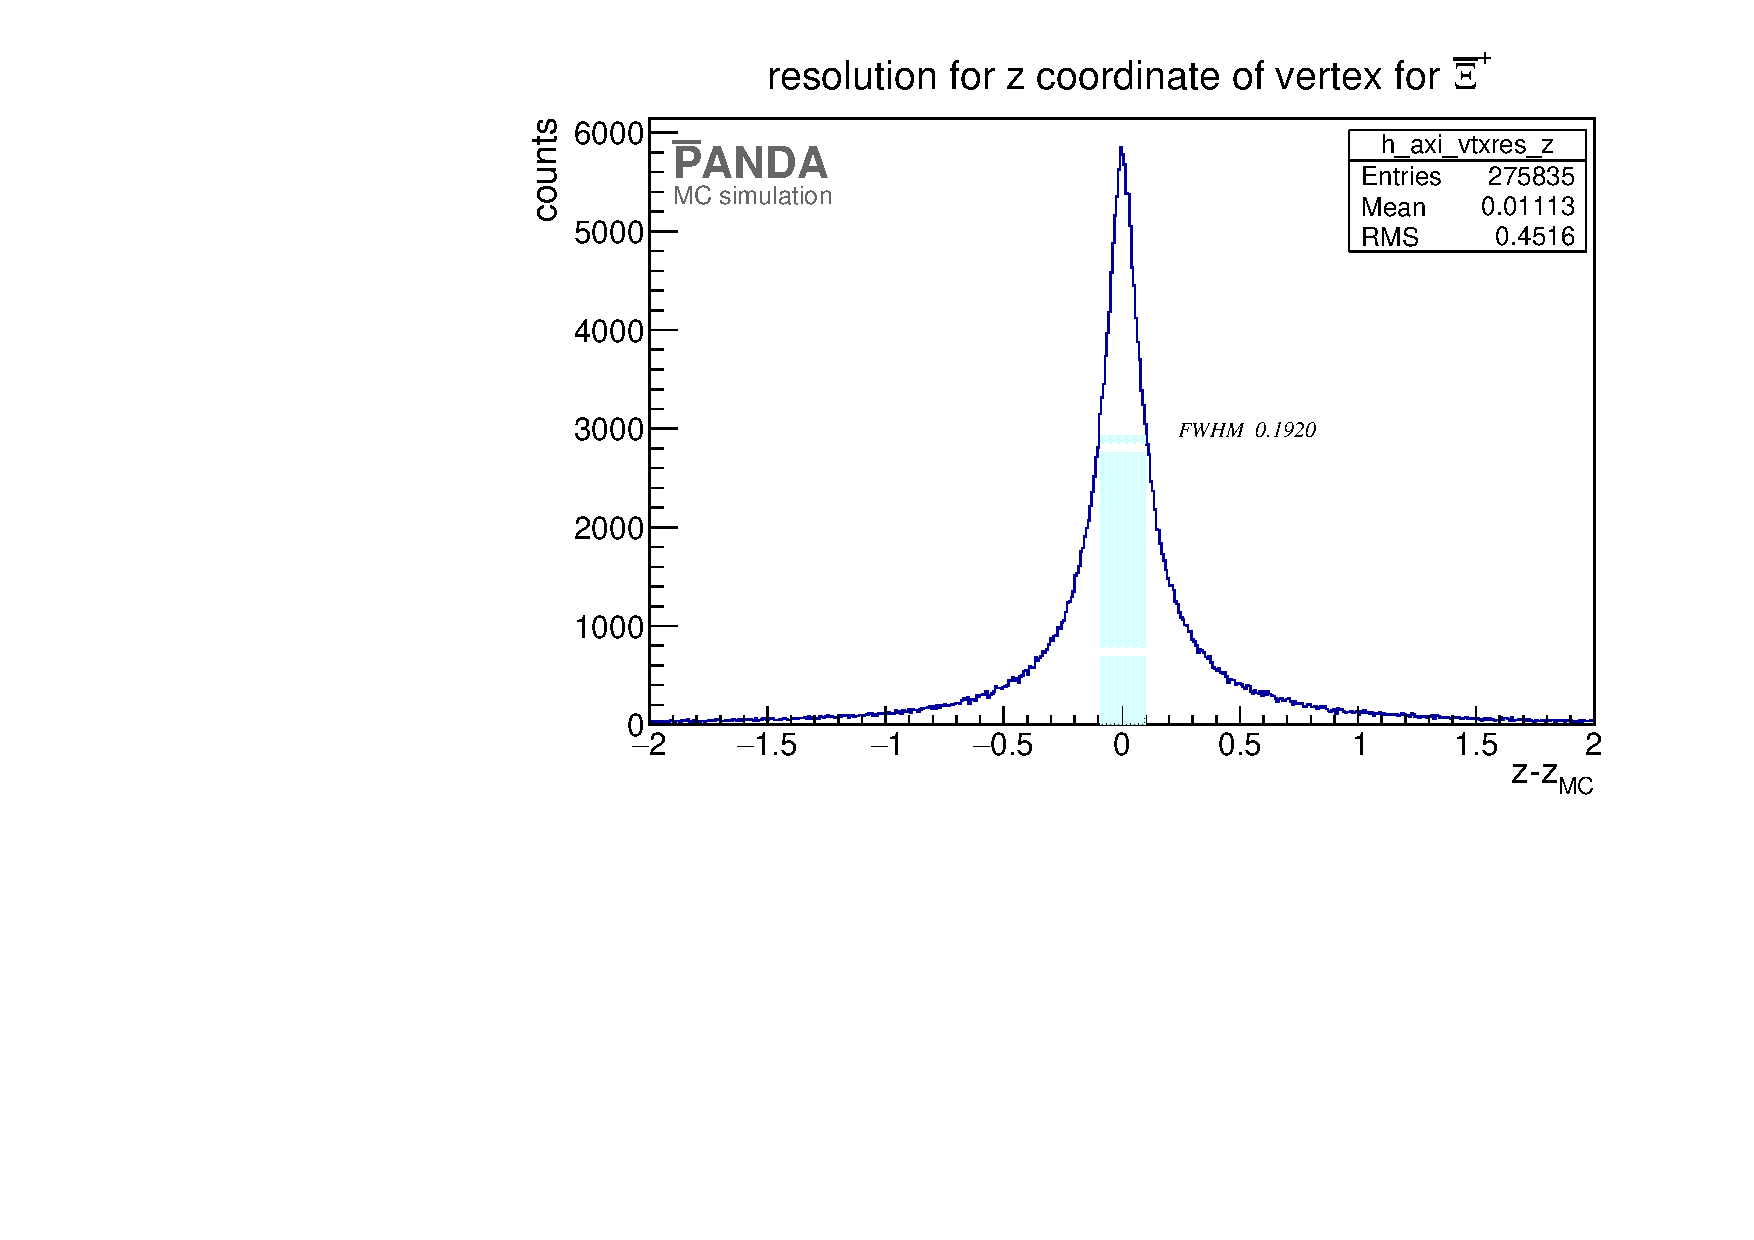
\includegraphics[width=0.49\textwidth]{./plots/Xi/XiPlus_vtxres_z.pdf}}
			\caption{\propose The left plot shows the vertex resolution of y position for \anticascade. The right plot shows the vertex
					 resolution of z position for \anticascade.}
			\label{fig:xi_vtxres_yz}
			
		\end{figure}
	
		The mass distribution for the different cuts is shown in figure \ref{fig:XiPlus_massdiffcuts} and figure \ref{fig:XiMinus_massdiffcuts}.
		The number of events is strongly reduced by the cut on the vertex fit probability. 
		The width of the mass distribution gets smaller. 
		
		\begin{figure}
			\centering
				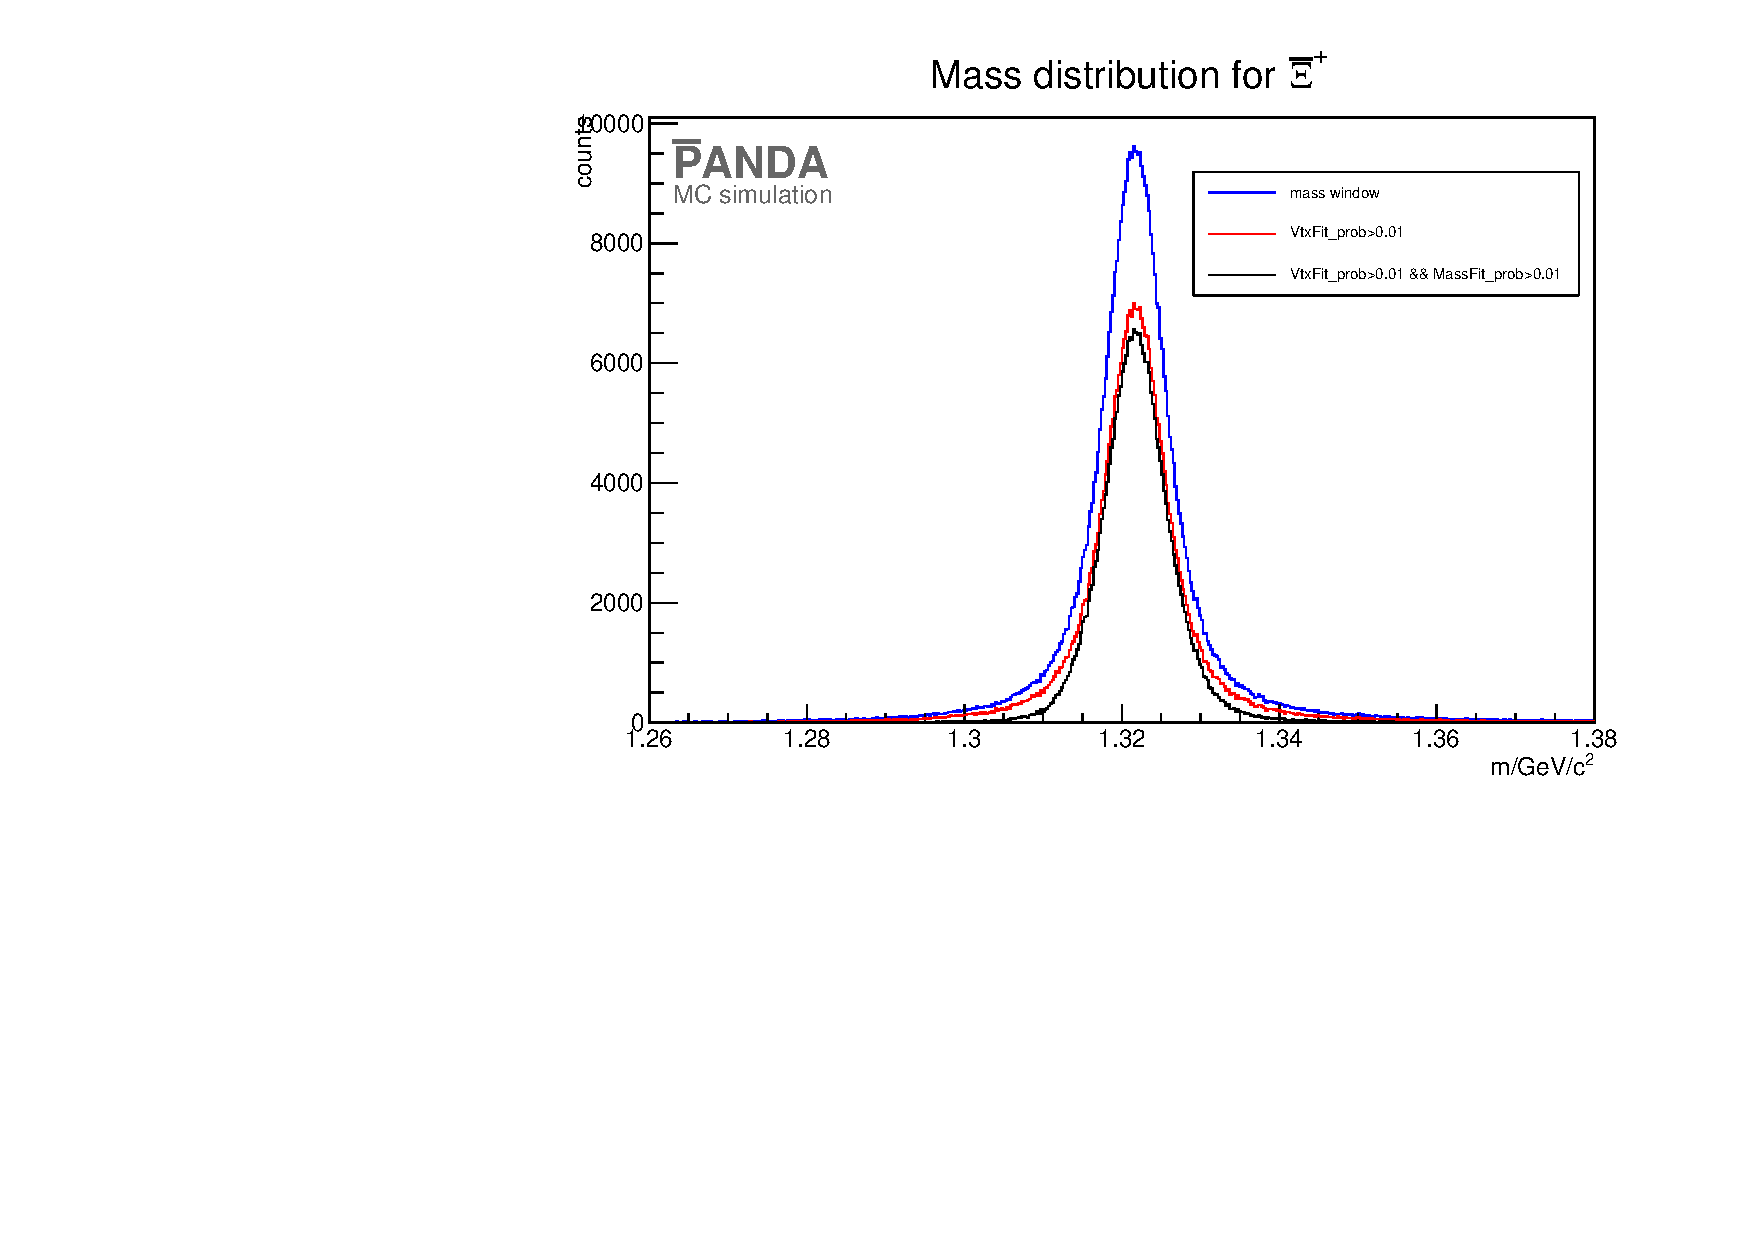
\includegraphics[width=1.1\textwidth]{./plots/Xi/XiPlus_m_diffcuts.pdf}
			\caption{\propose Mass distribution of \anticascade for different cuts: the mass window cut is shown in blue, the vertex fit cut is shown in red 
					and the distribution after all cuts is shown in black.}
			\label{fig:XiPlus_massdiffcuts}
		\end{figure}
		
		\begin{figure}
			\centering		
				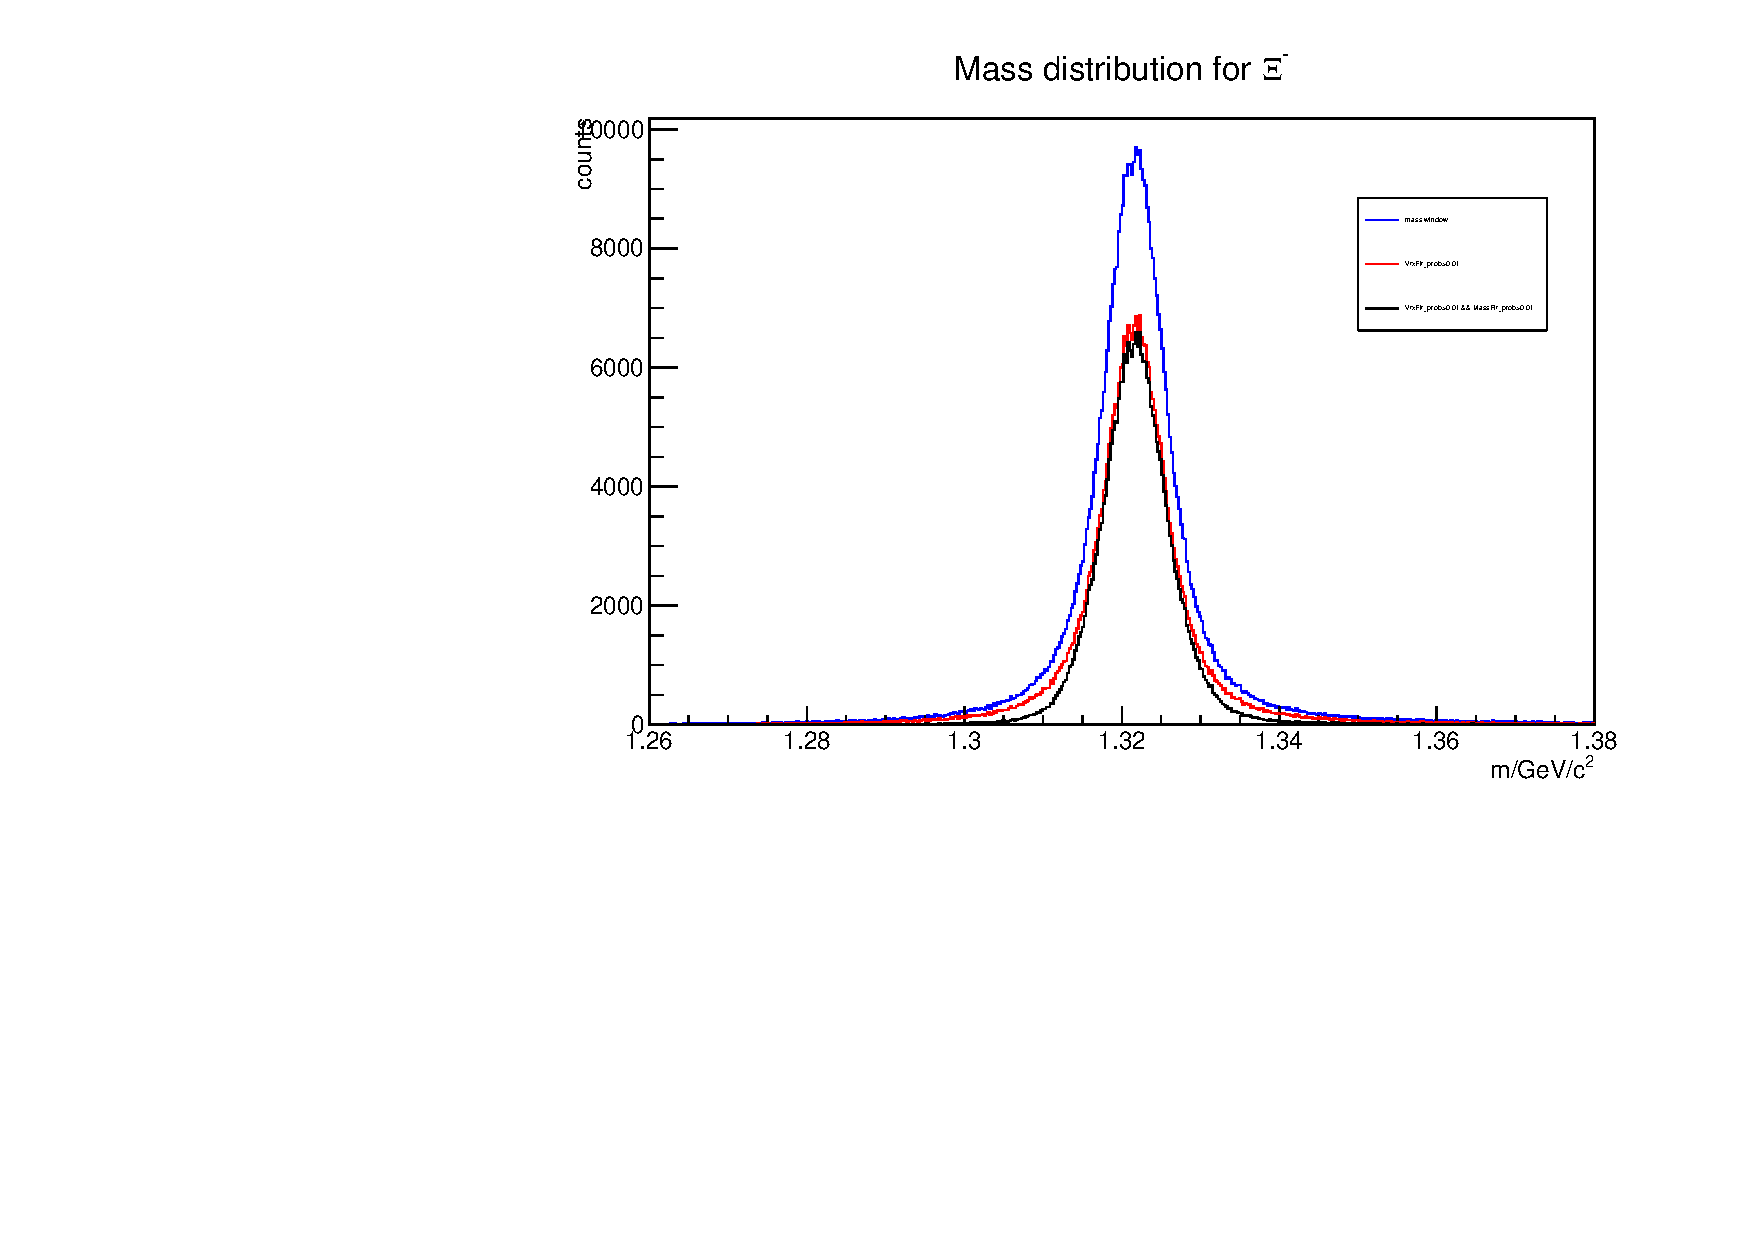
\includegraphics[width=1.1\textwidth]{./plots/Xi/XiMinus_m_diffcuts.pdf}
			\caption{\propose Mass distribution of \cascade for different cuts: mass window cut in blue, vertex fit cut in red and all cuts in black.}
			\label{fig:XiMinus_massdiffcuts}
		\end{figure}
		
		After using all cuts on the mass distribution the reconstructed mass of \cascade and \anticascade can be determined by a double Gaussian fit.
		This is exemplarily shown for the \cascade in figure \ref{fig:XiPlus_massfit}.
		
		\begin{figure}
			\centering
				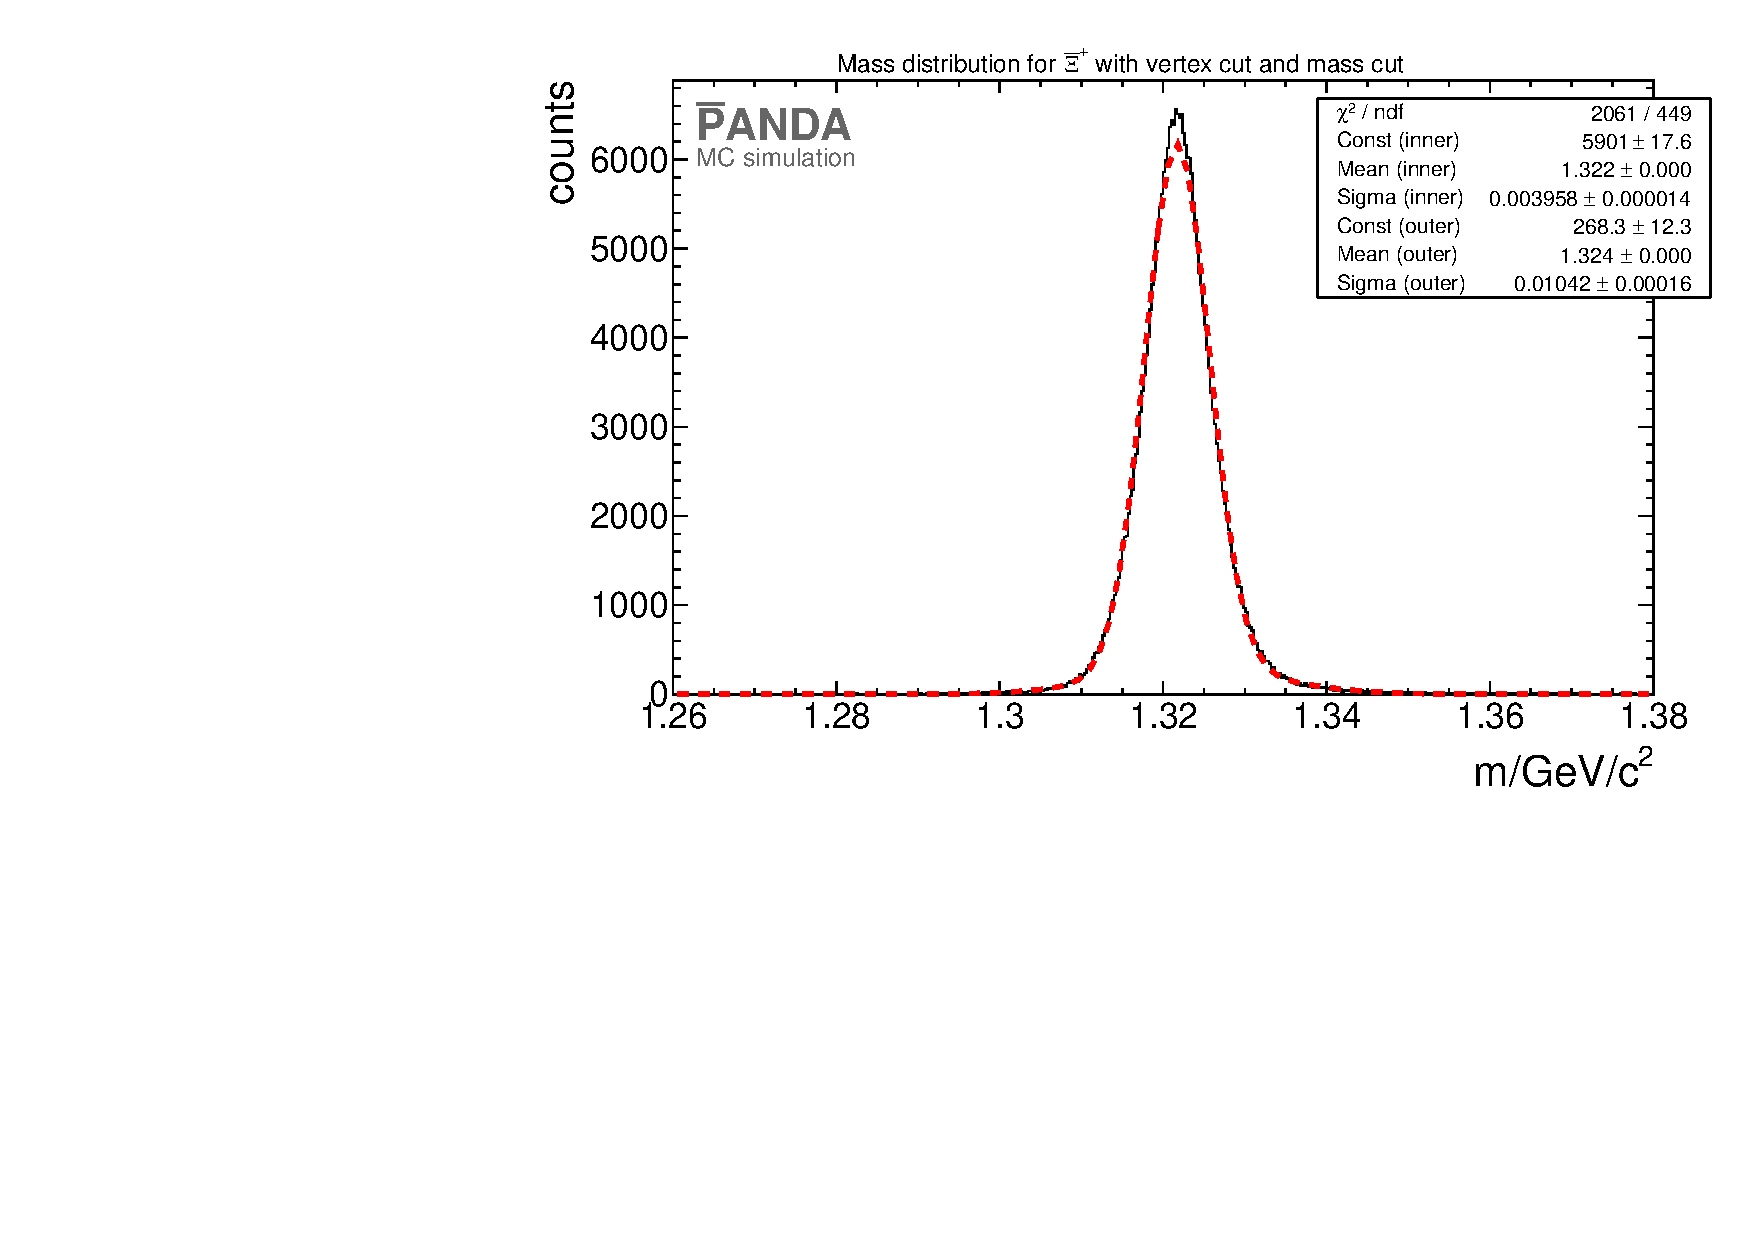
\includegraphics[width=0.8\textwidth]{./plots/Xi/XiPlus_m_masscut.pdf}
			\caption{\propose The plot shows the mass distribution (blue line) after all cuts. 
					A double Gaussian fit (red dashed line) is performed to determine the reconstructed mass for the \anticascade. }
			\label{fig:XiPlus_massfit}
		\end{figure}
		The result of the mass fit is for \anticascade ${\mt{m} = \left( 1.32172 \pm 0.00396\right)}$ \massunit 
		and for \cascade \\ ${\mt{m} = \left( 1.3216 \pm 0.004\right)}$\massunit.
		The two dimensional momentum distribution for \anticascade and \cascade is shown in figure \ref{fig:XiPlus_pt_vs_pz} 
		
		\begin{figure}
			\subfigure[\anticascade]{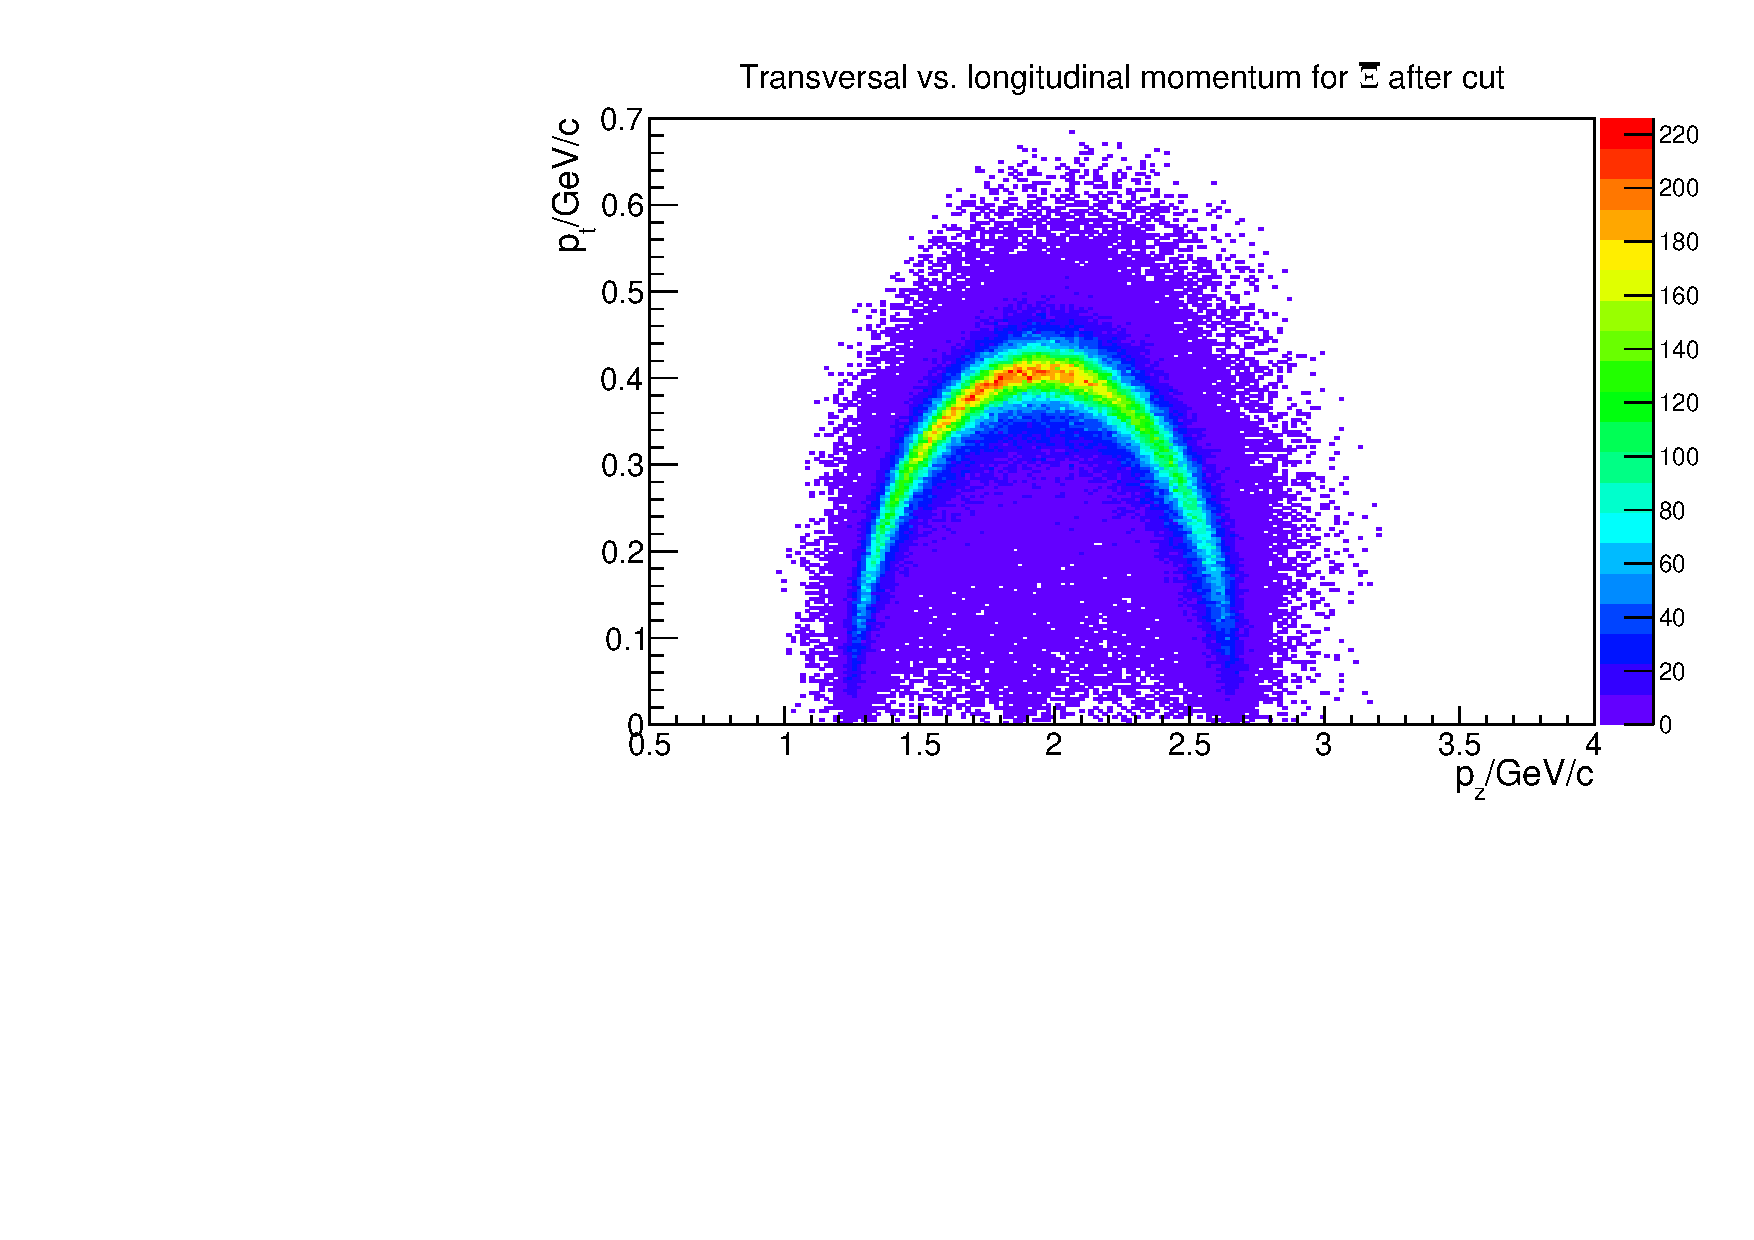
\includegraphics[width=0.49\textwidth]{./plots/Xi/XiPlus_pt_vs_pz_cut.pdf}}
			\subfigure[\cascade]{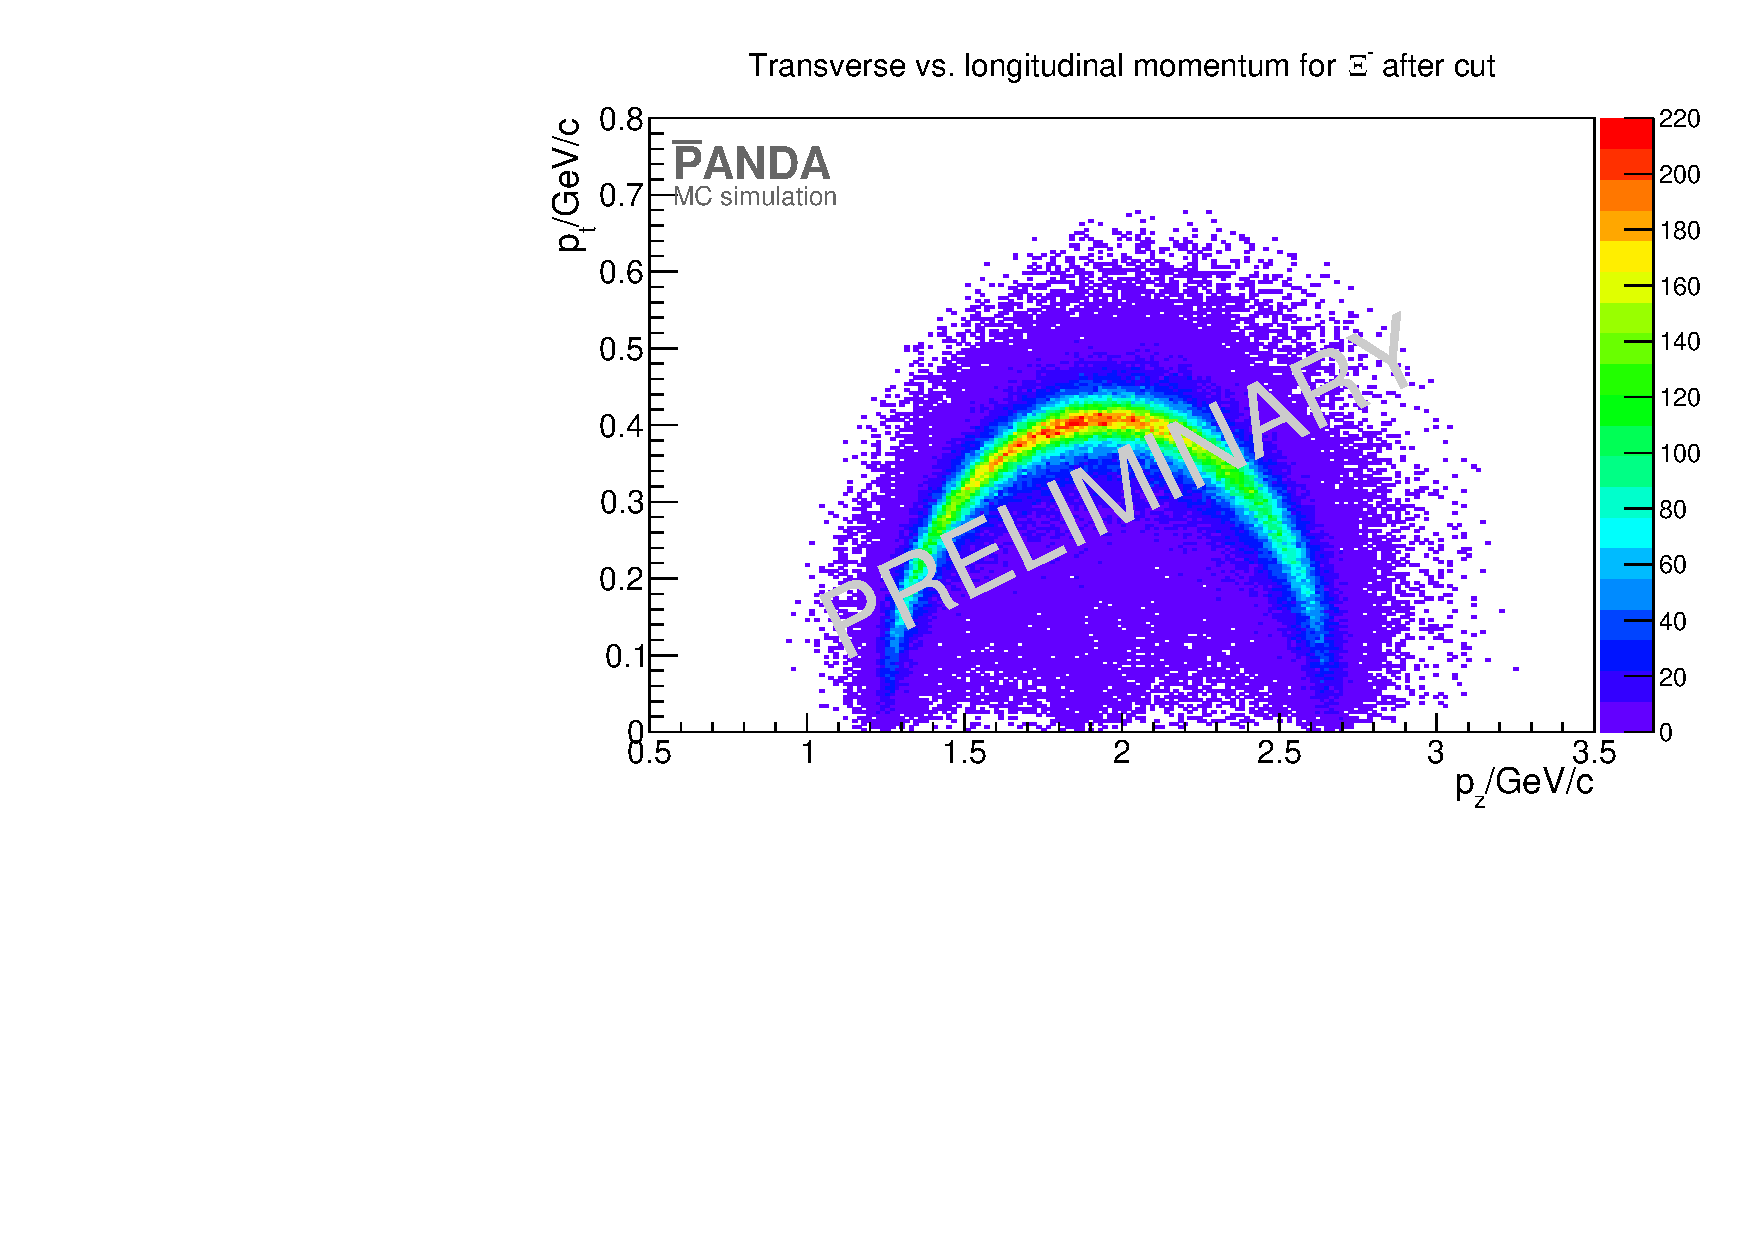
\includegraphics[width=0.49\textwidth]{./plots/Xi/XiMinus_pt_vs_pz_cut.pdf}}
			\caption{\propose The plots shows the transverse against the longitudinal momentum for \anticascade and \cascade}
			\label{fig:XiPlus_pt_vs_pz}
		
		\end{figure}
		
		The reconstruction efficiency for \anticascade is $18.39\%$ and for \cascade $18.64\%$.
		
	
	
	

\section{Reconstruction of \excitedcascade and \excitedanticascade}
		\subsection*{Selection}

		For the reconstruction of \excitedcascade one combines \lam with the \kminus meson and for \excitedanticascade \alam and \kplus using the
		best candidate from \lam and \alam.
		After the combination of the particles a mass window cut with width of $0.3$\massunit is performed. 
		The daughter particles are fitted then to a common vertex point with the PndKinVtxFitter.
		Only those candidates for \excitedcascade (\excitedanticascade) are selected which have a fit probability of more then $1\%$.
		The selection scheme is shown in figure \ref{fig:excitedcascade_scheme}. 
		
		\begin{figure}
			\centering
				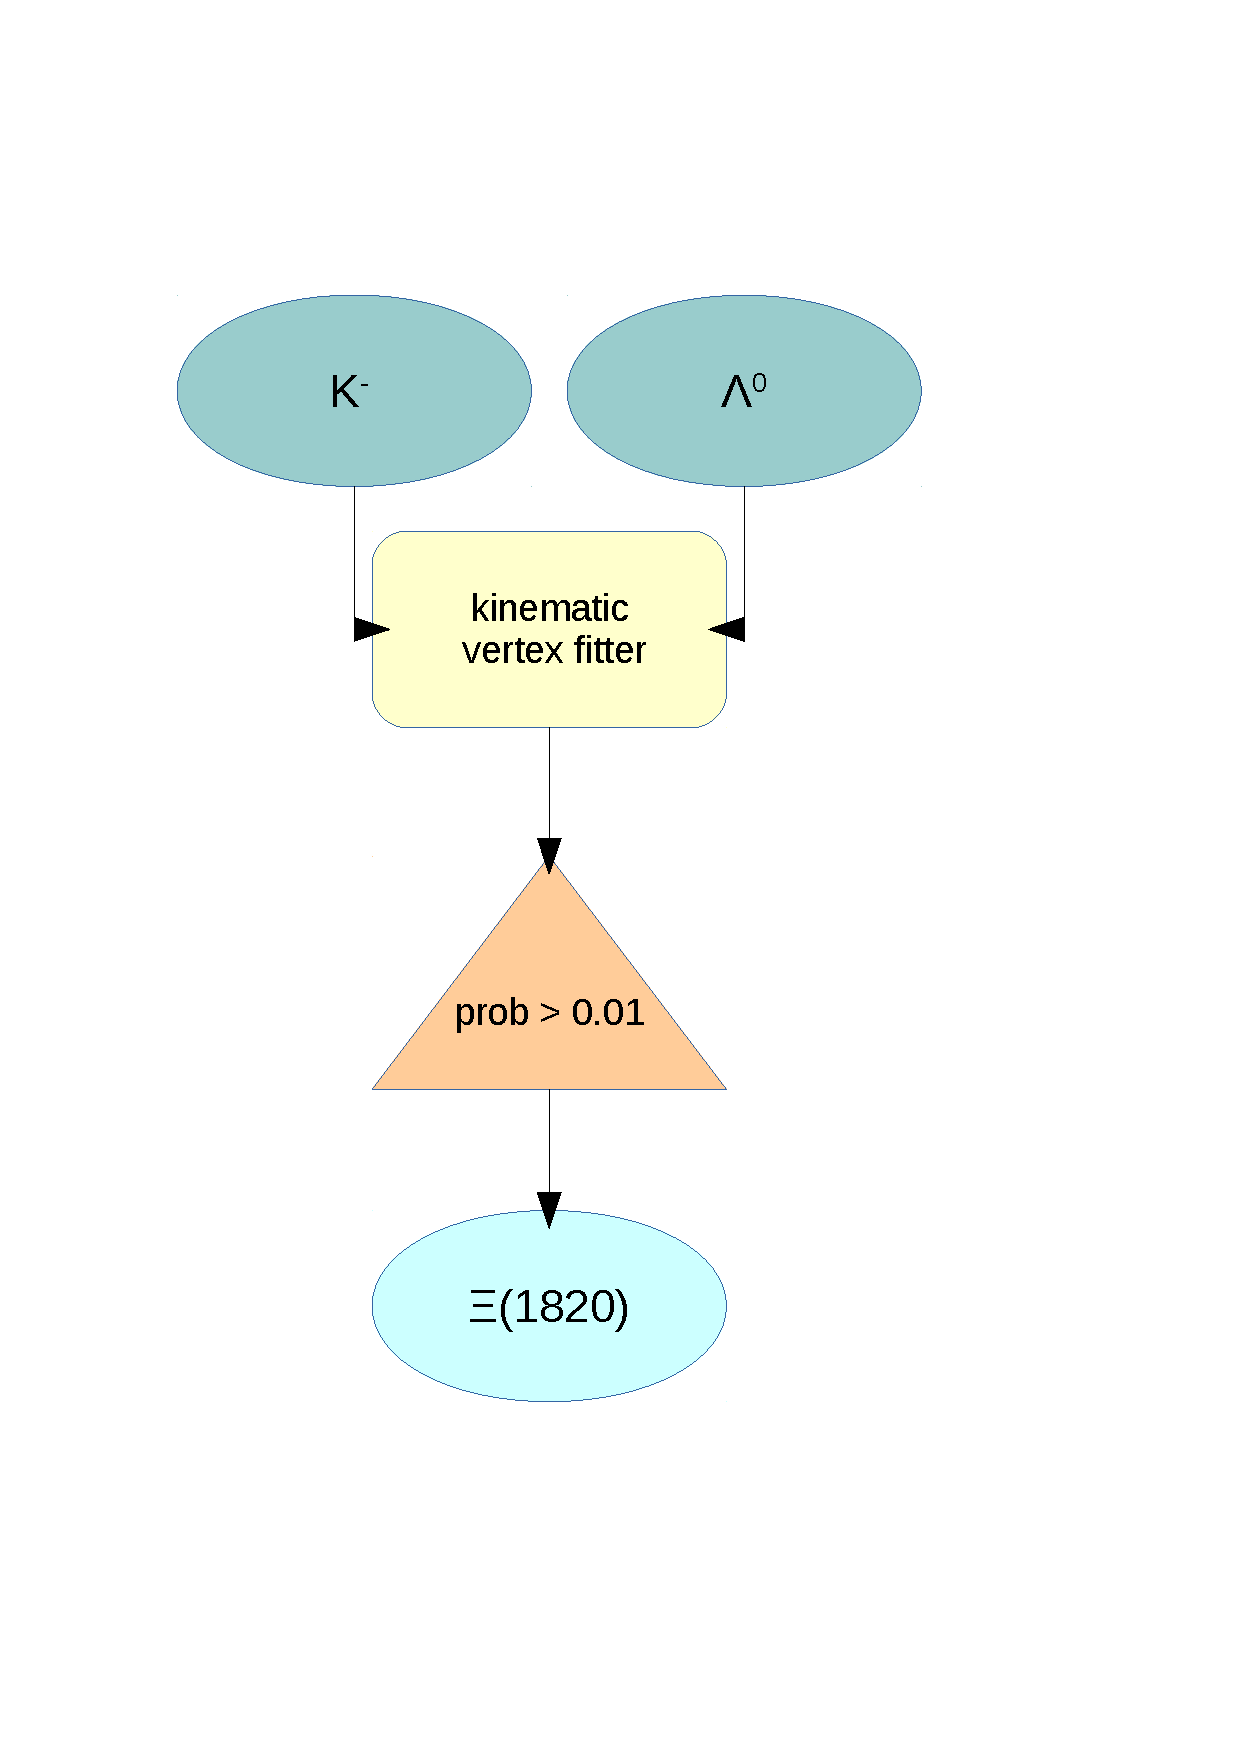
\includegraphics[width=0.50\textwidth]{./plots/combineExcitedCascade.pdf}
			\caption{\propose Scheme for \excitedcascade reconstruction}
			\label{fig:excitedcascade_scheme}
		\end{figure}
		
		
		The \chisq probability distribution for the vertex fit is shown in figure \ref{fig:xi1820_prob}.
		The distribution is again not flat but increases for values up to one. 
		
		\begin{figure}
			\centering
			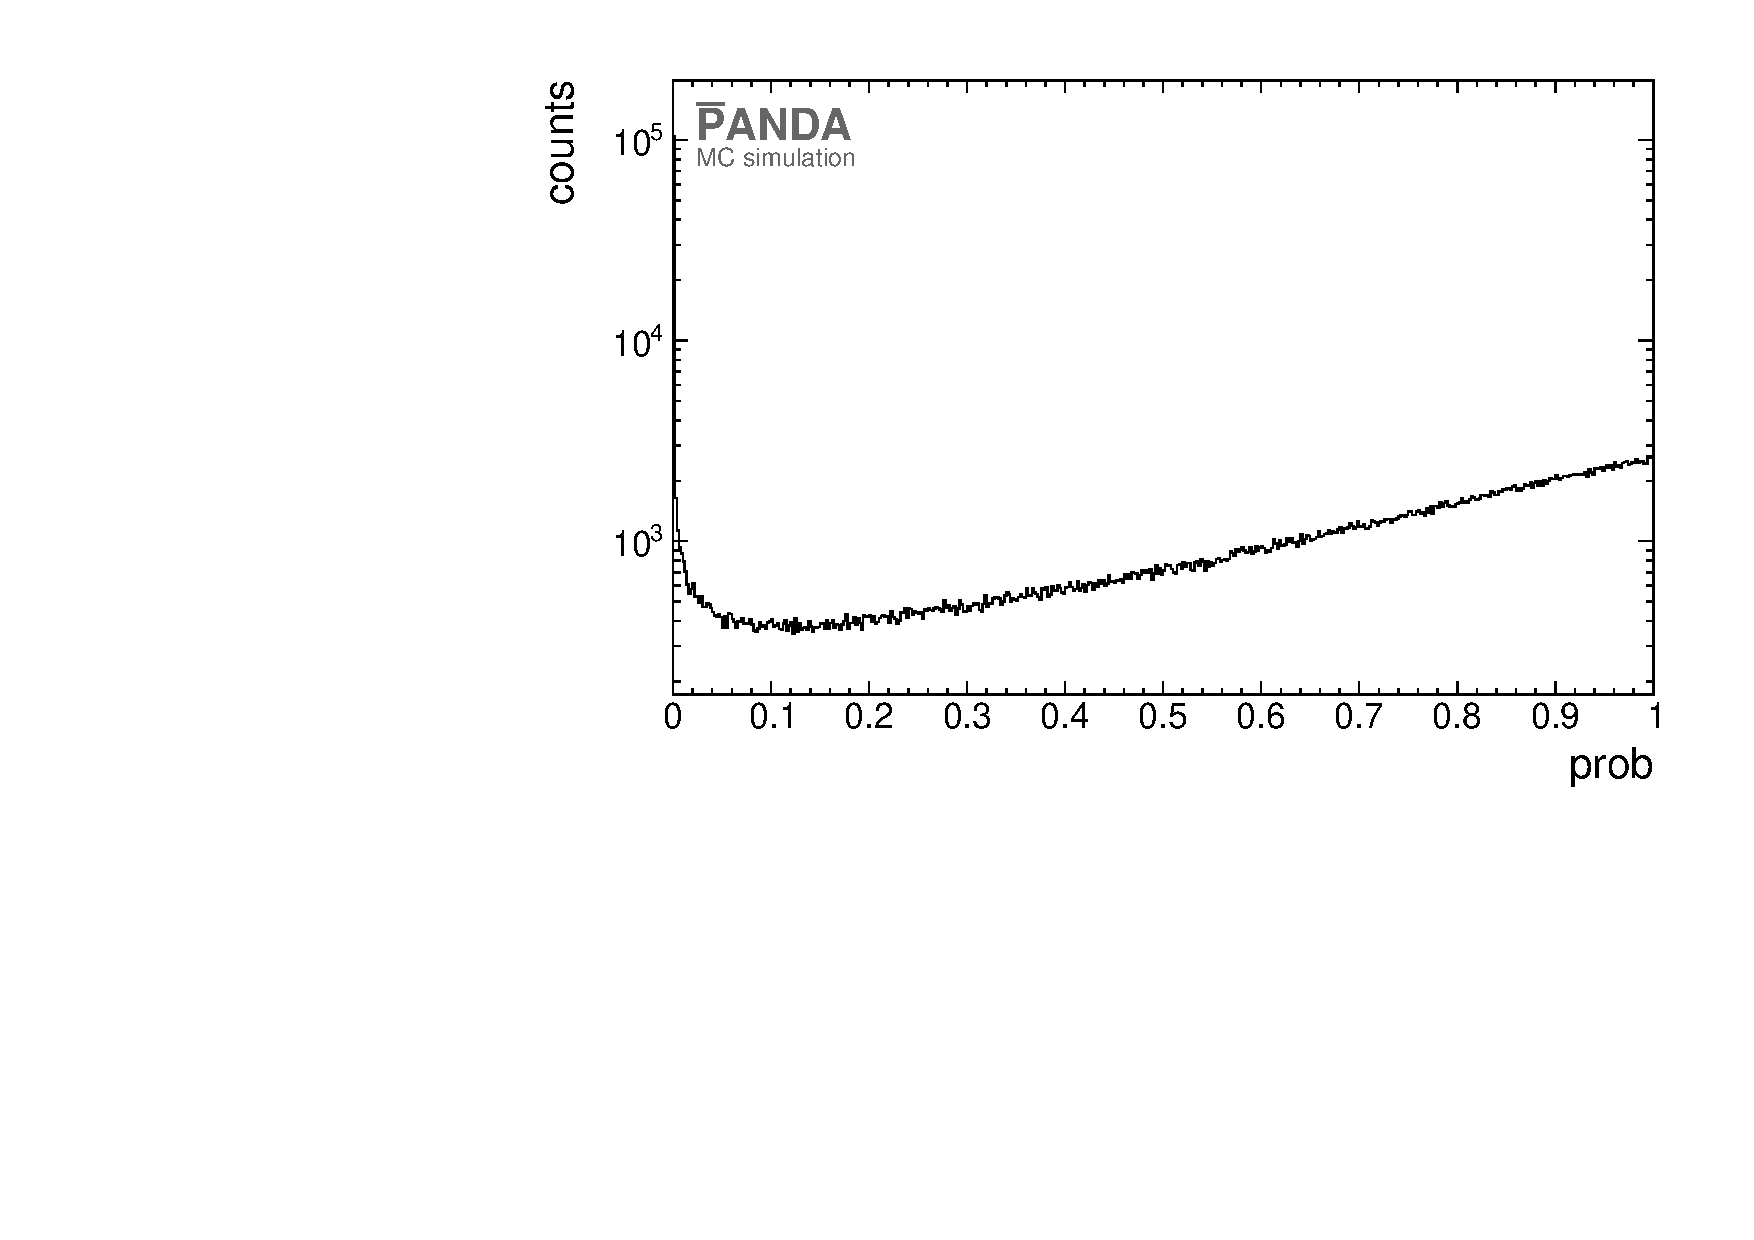
\includegraphics[width=1.\textwidth]{./plots/Xi1820/XiMinus1820_prob.pdf}
			\caption{\propose \chisq probability distribution of kinematic vertex fit for \excitedcascade.}
			\label{fig:xi1820_prob}
		\end{figure}
		
		If there is more than one particle the best candidate is chosen.
		
	\subsection*{Results}
	The vertex resolution for \excitedcascade and \excitedanticascade is summarized in table \ref{tab:Xi1820_vtxres}.
	
	\begin{table}
		\centering
		\caption{\propose Vertex resolution for \excitedcascade and \excitedanticascade.}
		\label{tab:Xi1820_vtxres}
		\begin{tabular}{ccc}
			\hline
			position & \excitedcascade & \excitedanticascade (from charge conjugate.) \\
			\hline
			\hline
			x/cm & 0.028 & 0.028\\
			y/cm & 0.028 & 0.028\\
			z/cm & 0.1 & 0.1\\
			\hline
			 
		\end{tabular}
	\end{table}
	
	Here again the vertex resolution is calculated with the FWHM. 
	This is exemplarily shown for \excitedcascade in figure \ref{fig:Xi1820_vtxx} and figure \ref{fig:Xi1820_vtxyz}.
	
	\begin{figure}
		\centering
		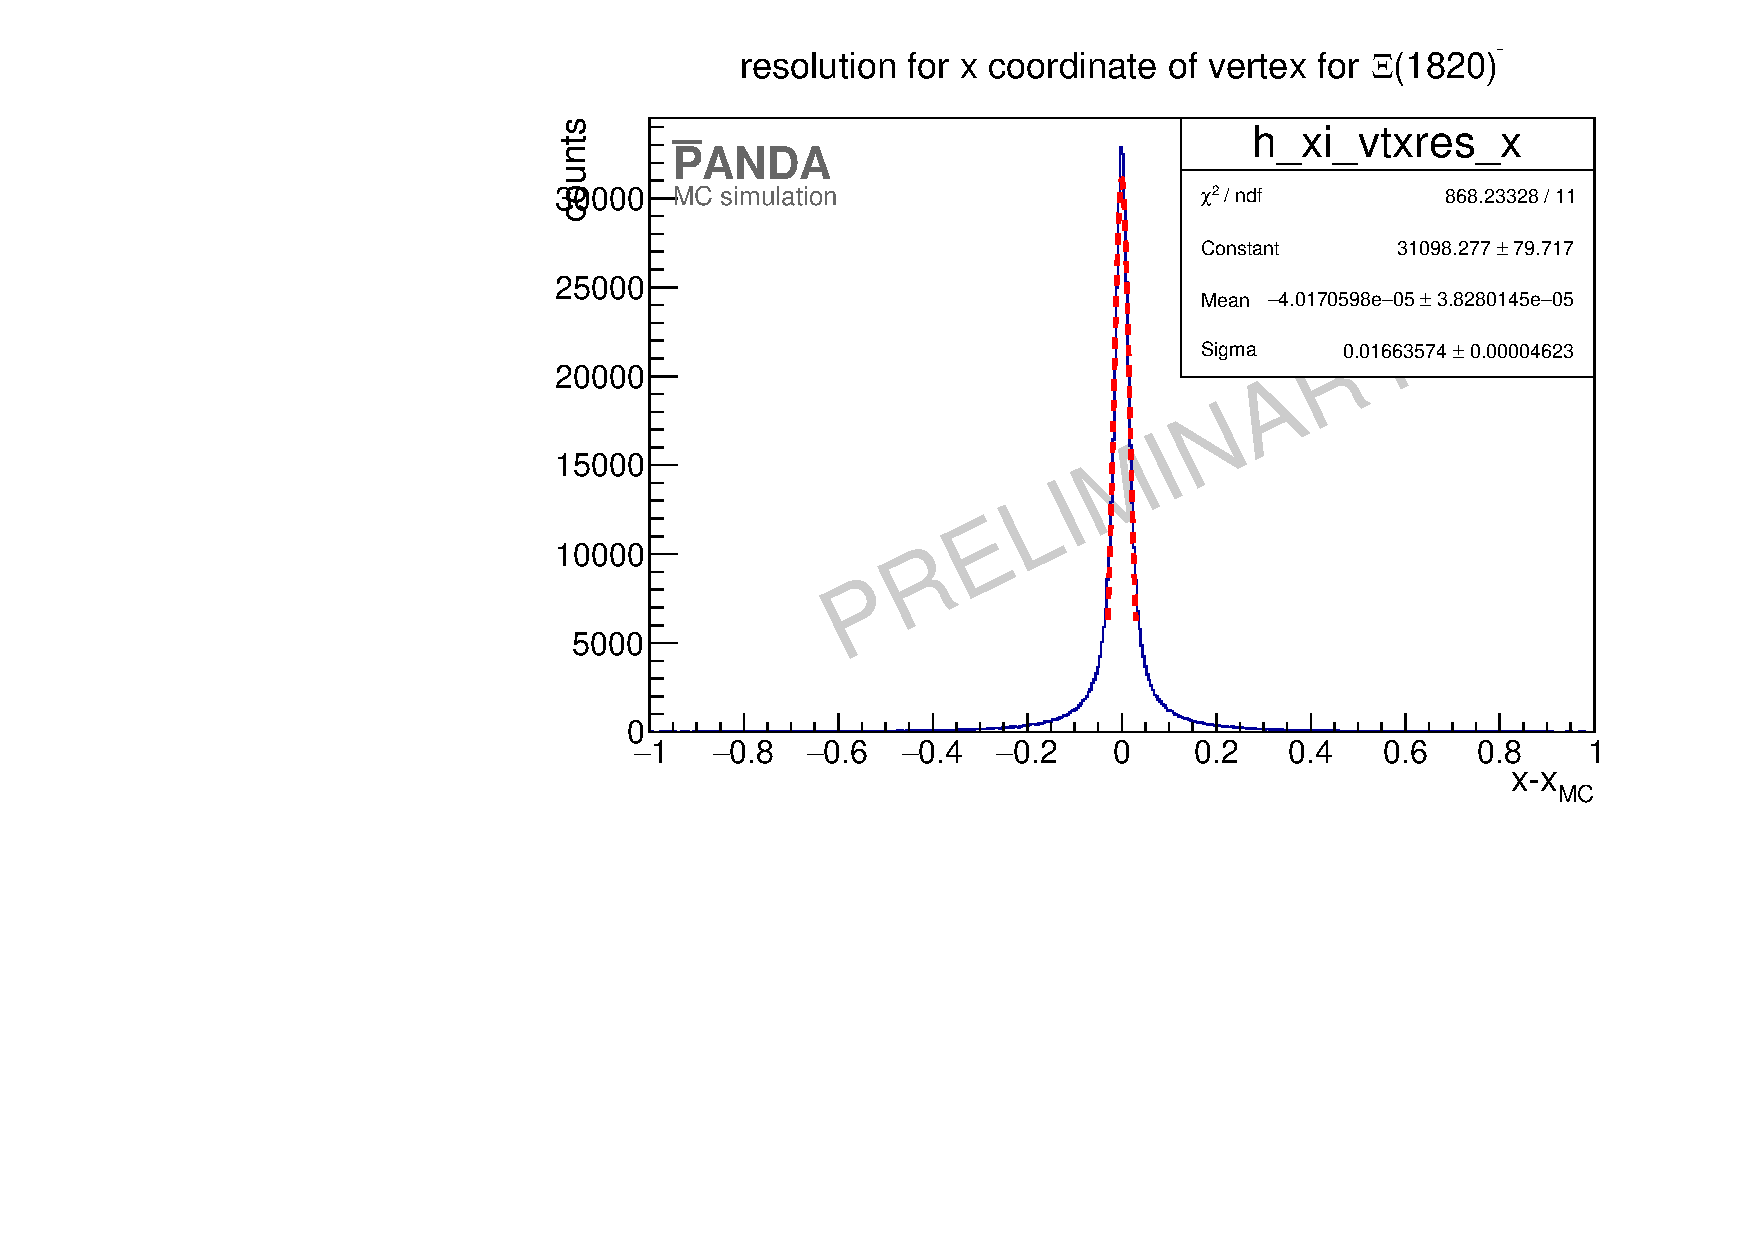
\includegraphics[width=0.7\textwidth]{./plots/Xi1820/XiMinus1820_vtxres_x.pdf}
		\caption{\propose Vertex resolution of the x coordinate for \excitedcascade.}
		\label{fig:Xi1820_vtxx}
	\end{figure}
	
	 \begin{figure}
		\centering
		\subfigure[Vertex resolution of the y coordinate for \excitedcascade.]{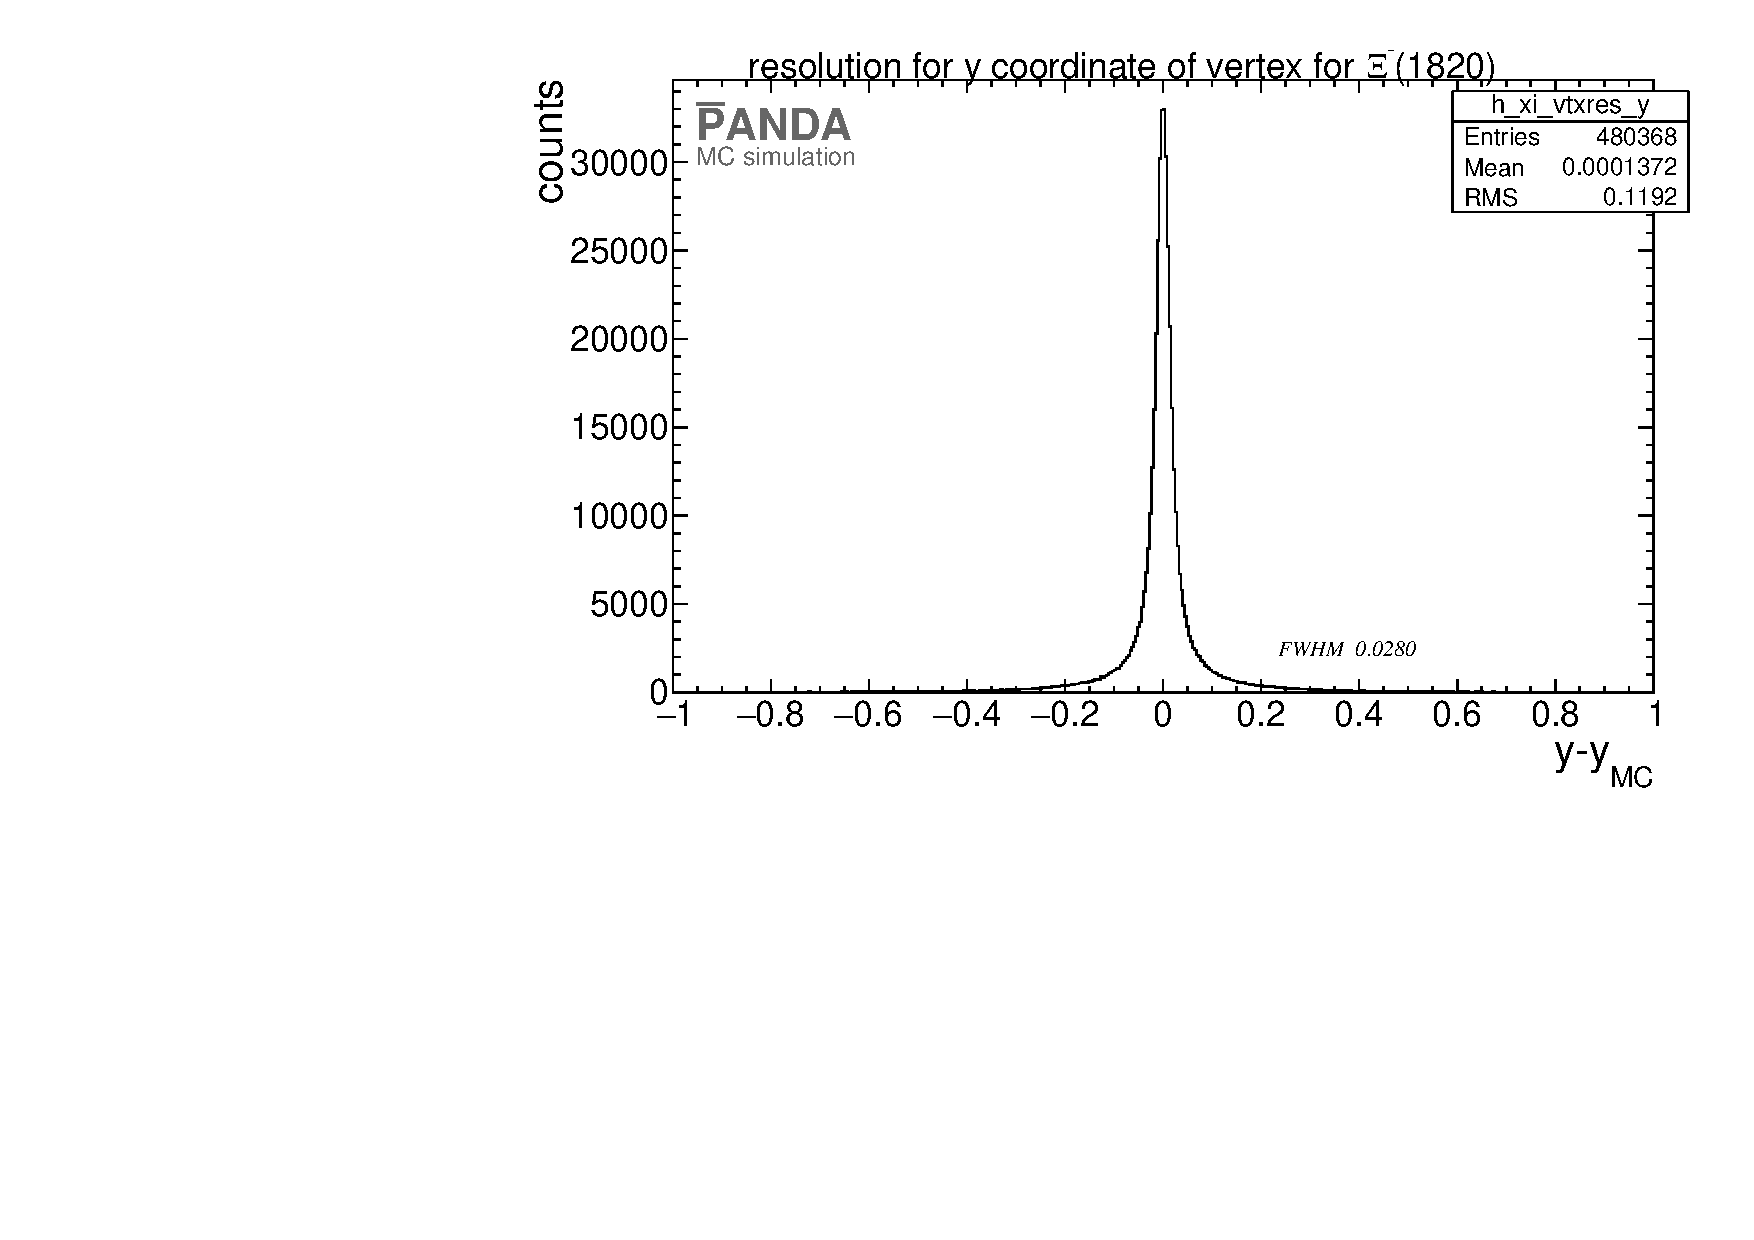
\includegraphics[width=0.49\textwidth]{./plots/Xi1820/XiMinus1820_vtxres_y.pdf}}
		\subfigure[Vertex resolution of the z coordinate for \excitedcascade.]{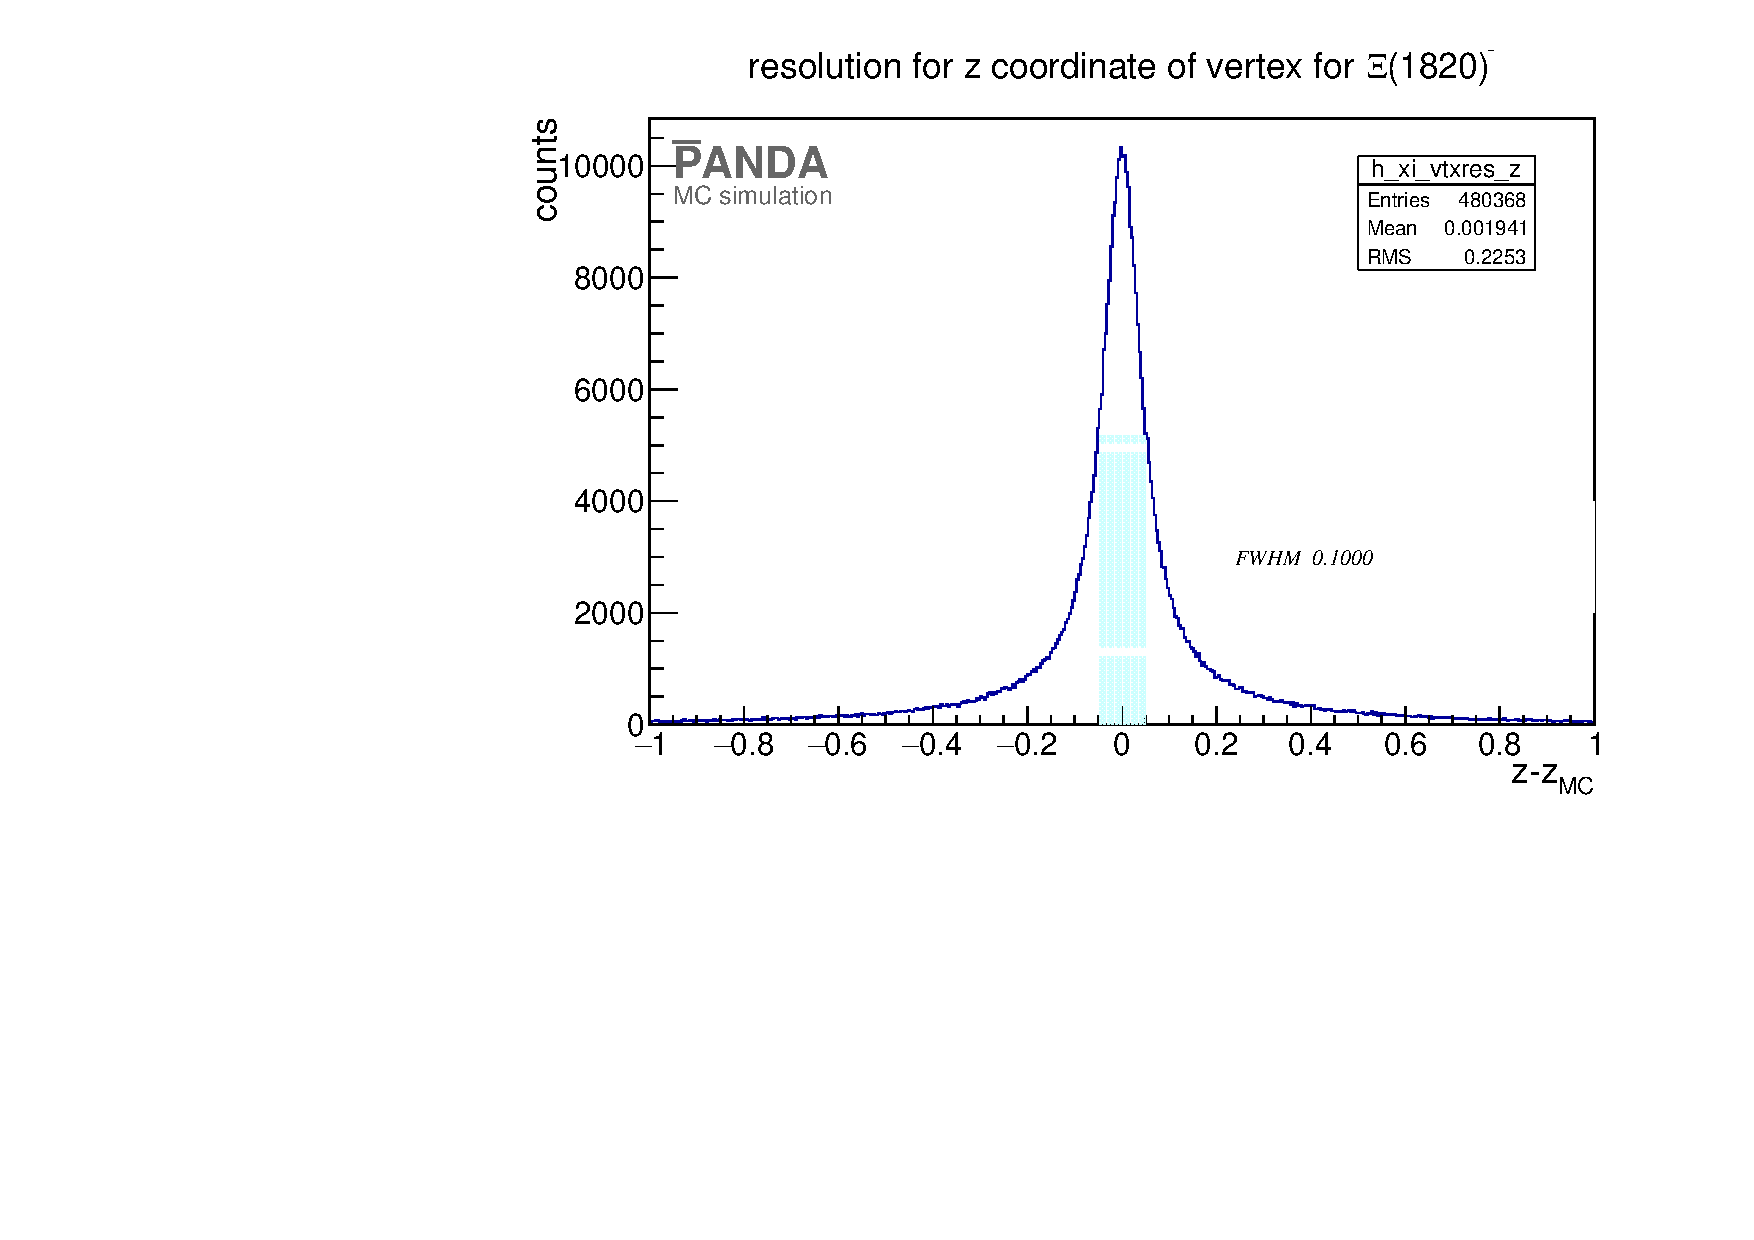
\includegraphics[width=0.49\textwidth]{./plots/Xi1820/XiMinus1820_vtxres_z.pdf}}
		\caption{\propose Figure a) shows the vertex resolution for the y coordinate and figure b) for the z coordinate of \excitedcascade}
		\label{fig:Xi1820_vtxyz}
	\end{figure}
	
	After performing both fits and cut on the probability values, the mass for \excitedcascade and \excitedanticascade
	can be determined by fitting with a double Gaussian function. 
	Figure \ref{fig:xi1820_mass_diffcuts} shows the mass distribution for both particles after each cut.
	
	\begin{figure}
		\centering
		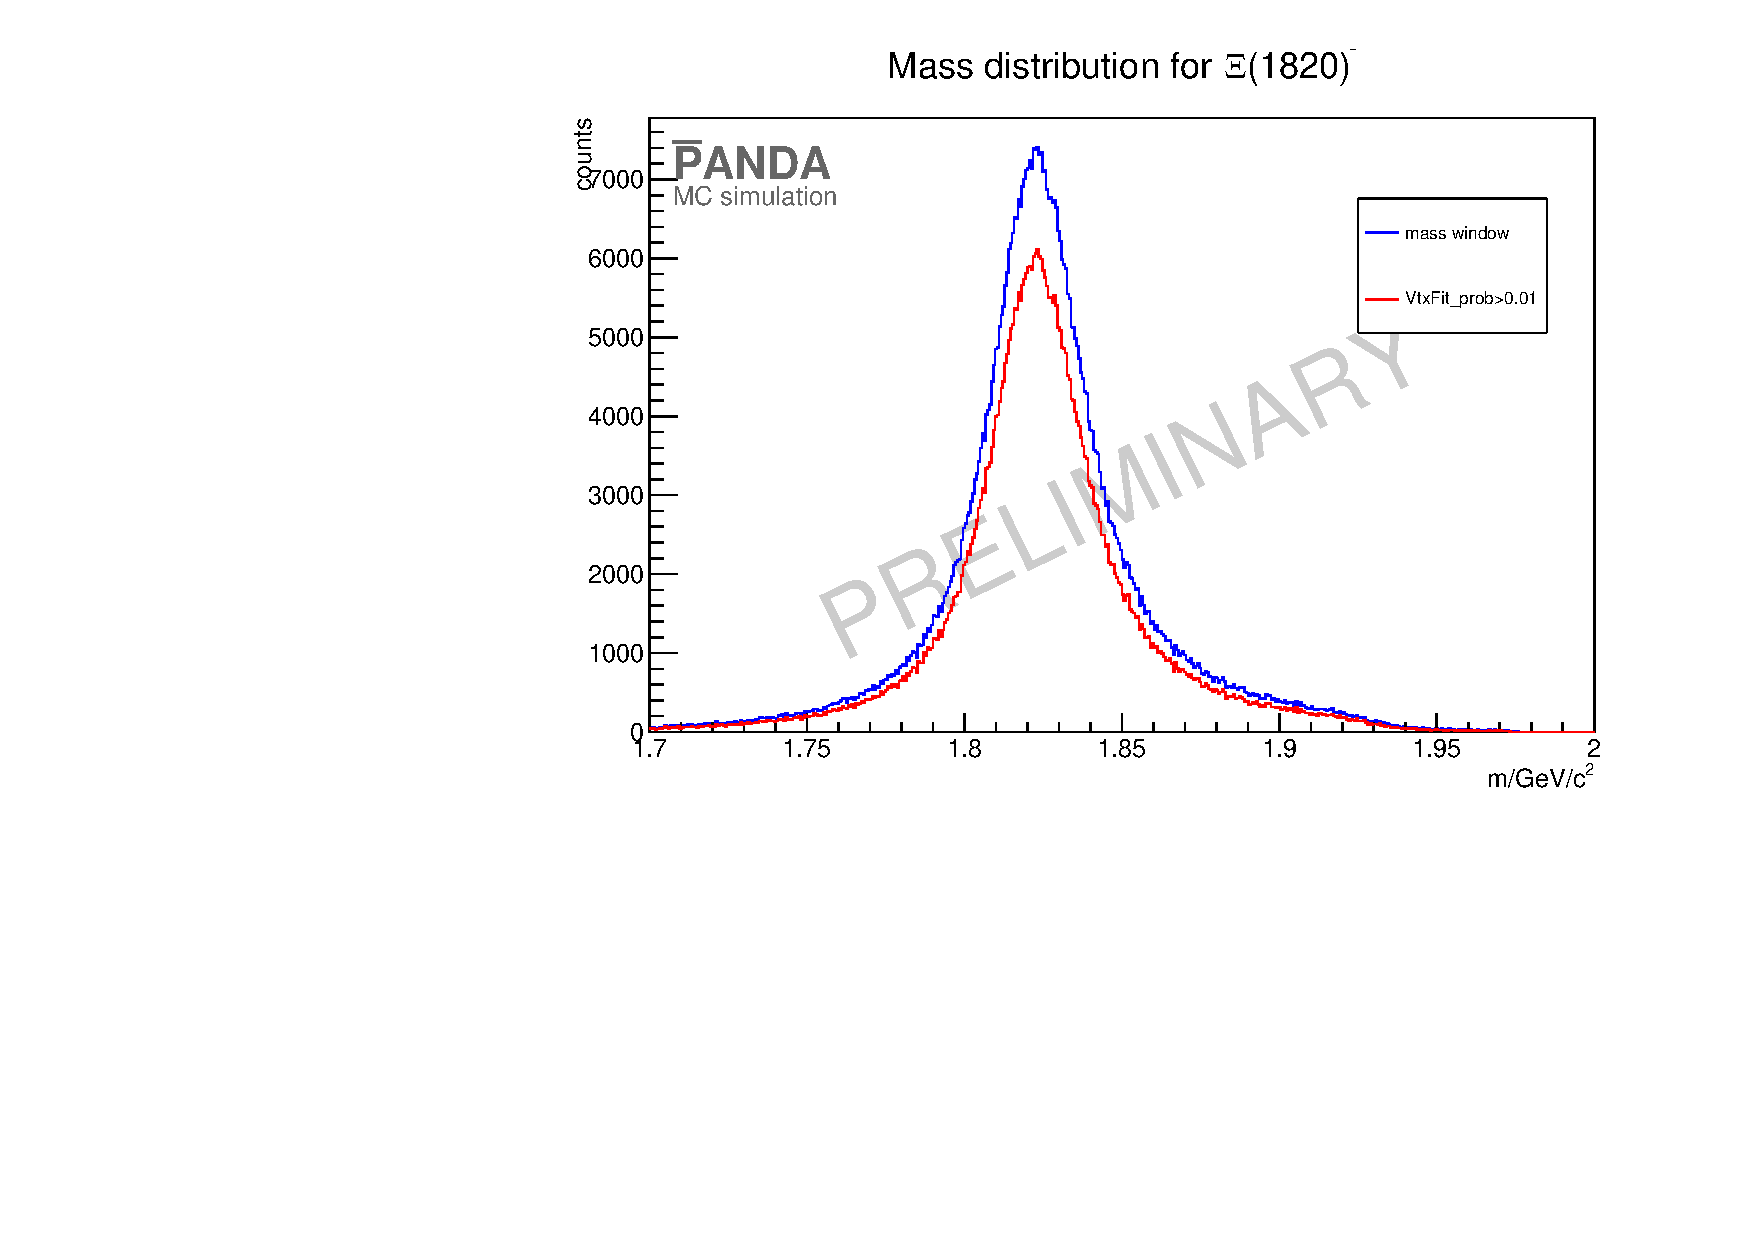
\includegraphics[width=1.\textwidth]{./plots/Xi1820/XiMinus1820_m_diffcuts.pdf}
		\caption{\propose Mass distribution for \excitedcascade after the mass window cut in blue and after the vertex fit probability cut in red.}
		\label{fig:xi1820_mass_diffcuts}
	
	\end{figure}
	The mass fit is exemplarily shown for the \excitedcascade in figure \ref{fig:xi1820_massfit}. 
	
	\begin{figure}
		\centering
		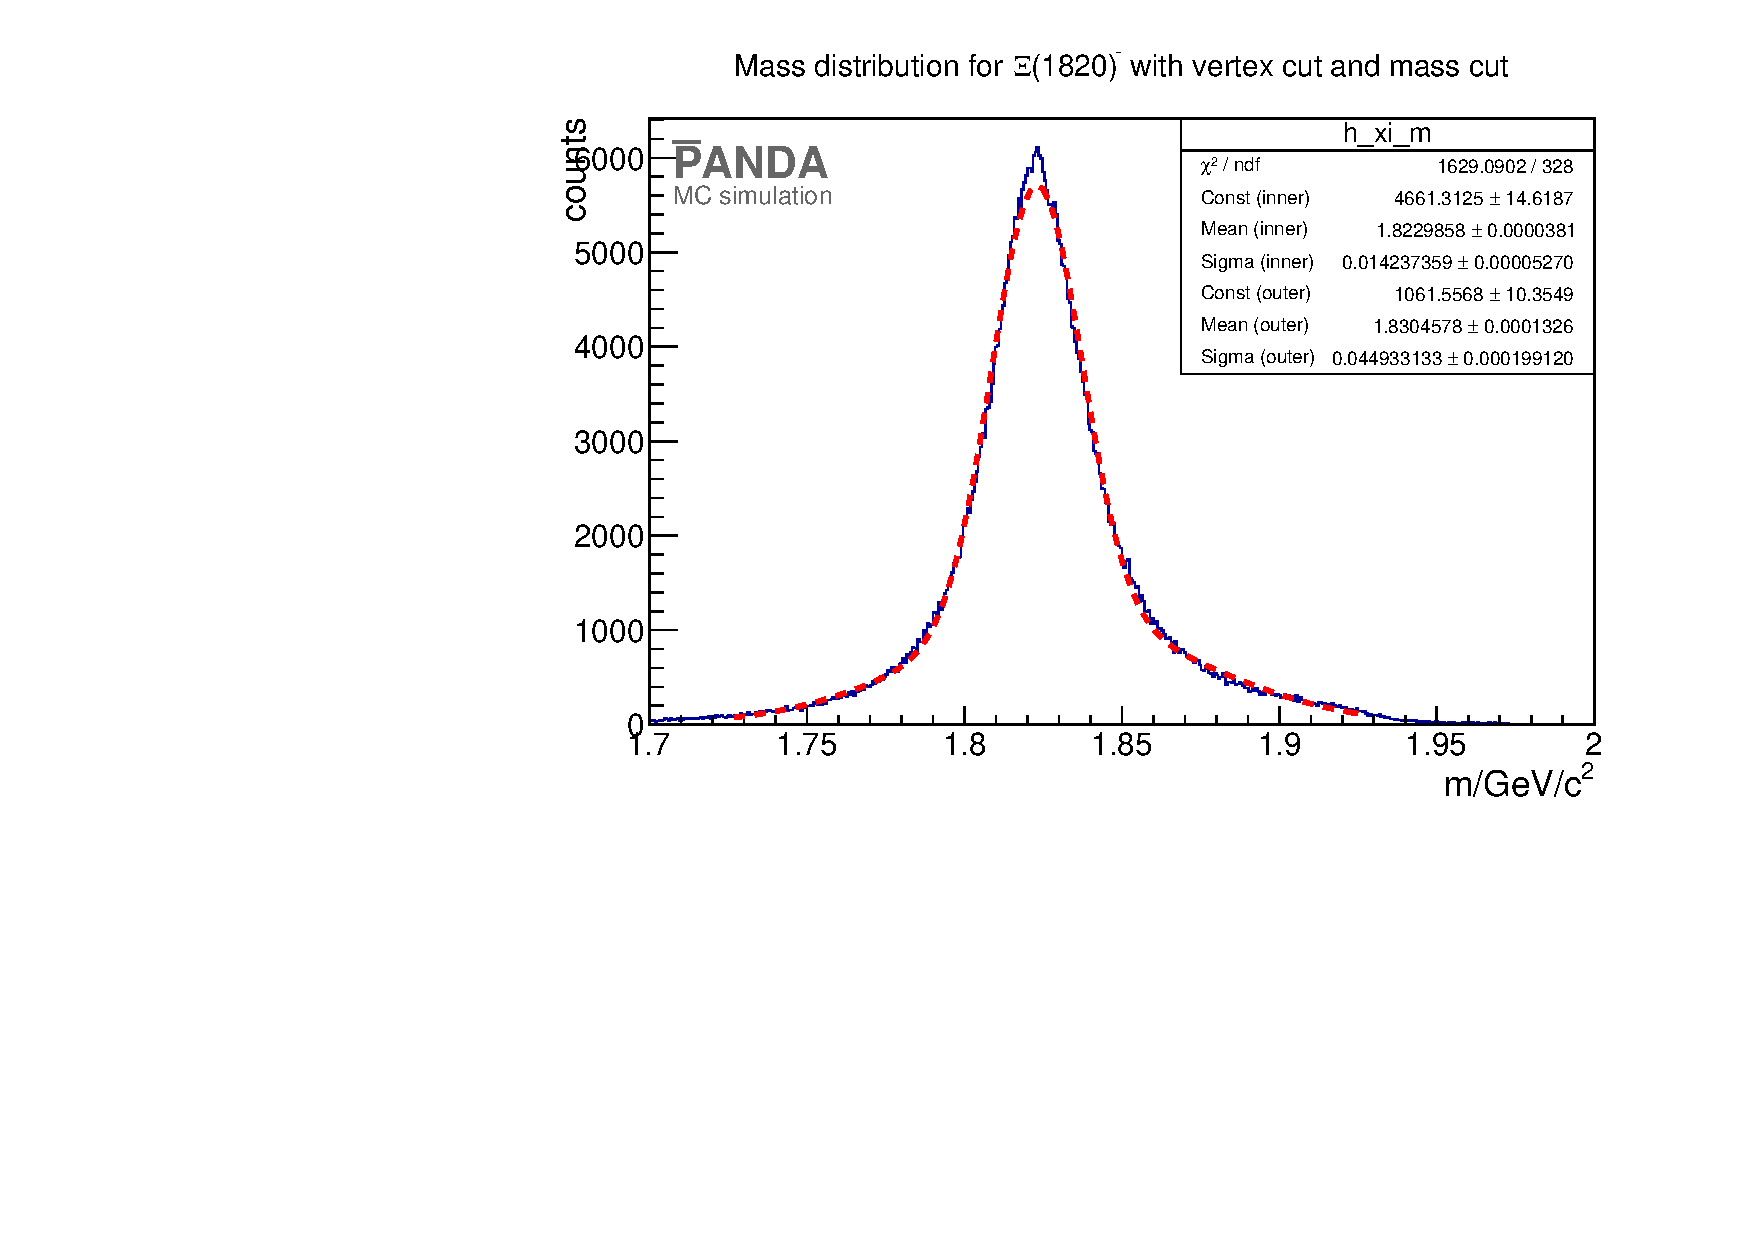
\includegraphics[width=1.\textwidth]{./plots/Xi1820/XiMinus1820_m_masscut.pdf}
		\caption{\propose Mass distribution (blue line) after all cuts for \excitedcascade. The performed double Gaussian fit is shown as red dashed line.}
		\label{fig:xi1820_massfit}
	\end{figure}
	The mass value for the \excitedcascade is fitted to $m_{\Xi^{*}} = 1.8229 \pm 3.81 \cdot 10^{-5}$ \massunit
	 and for \excitedanticascade to $m_{\bar{\Xi}^{*}} = 1.823 \pm 3.73\cdot 10^{-5}$ \massunit.
	These values are close to the input value.
	Figure \ref{fig:xi1820_pt_vs_pz} shows the two dimensional momentum distribution. For both subplots the x axis shows the longitudinal momentum
	and on the y axis there is shown the transverse momentum.
	
	\begin{figure}
		\centering
		\subfigure[\excitedcascade]{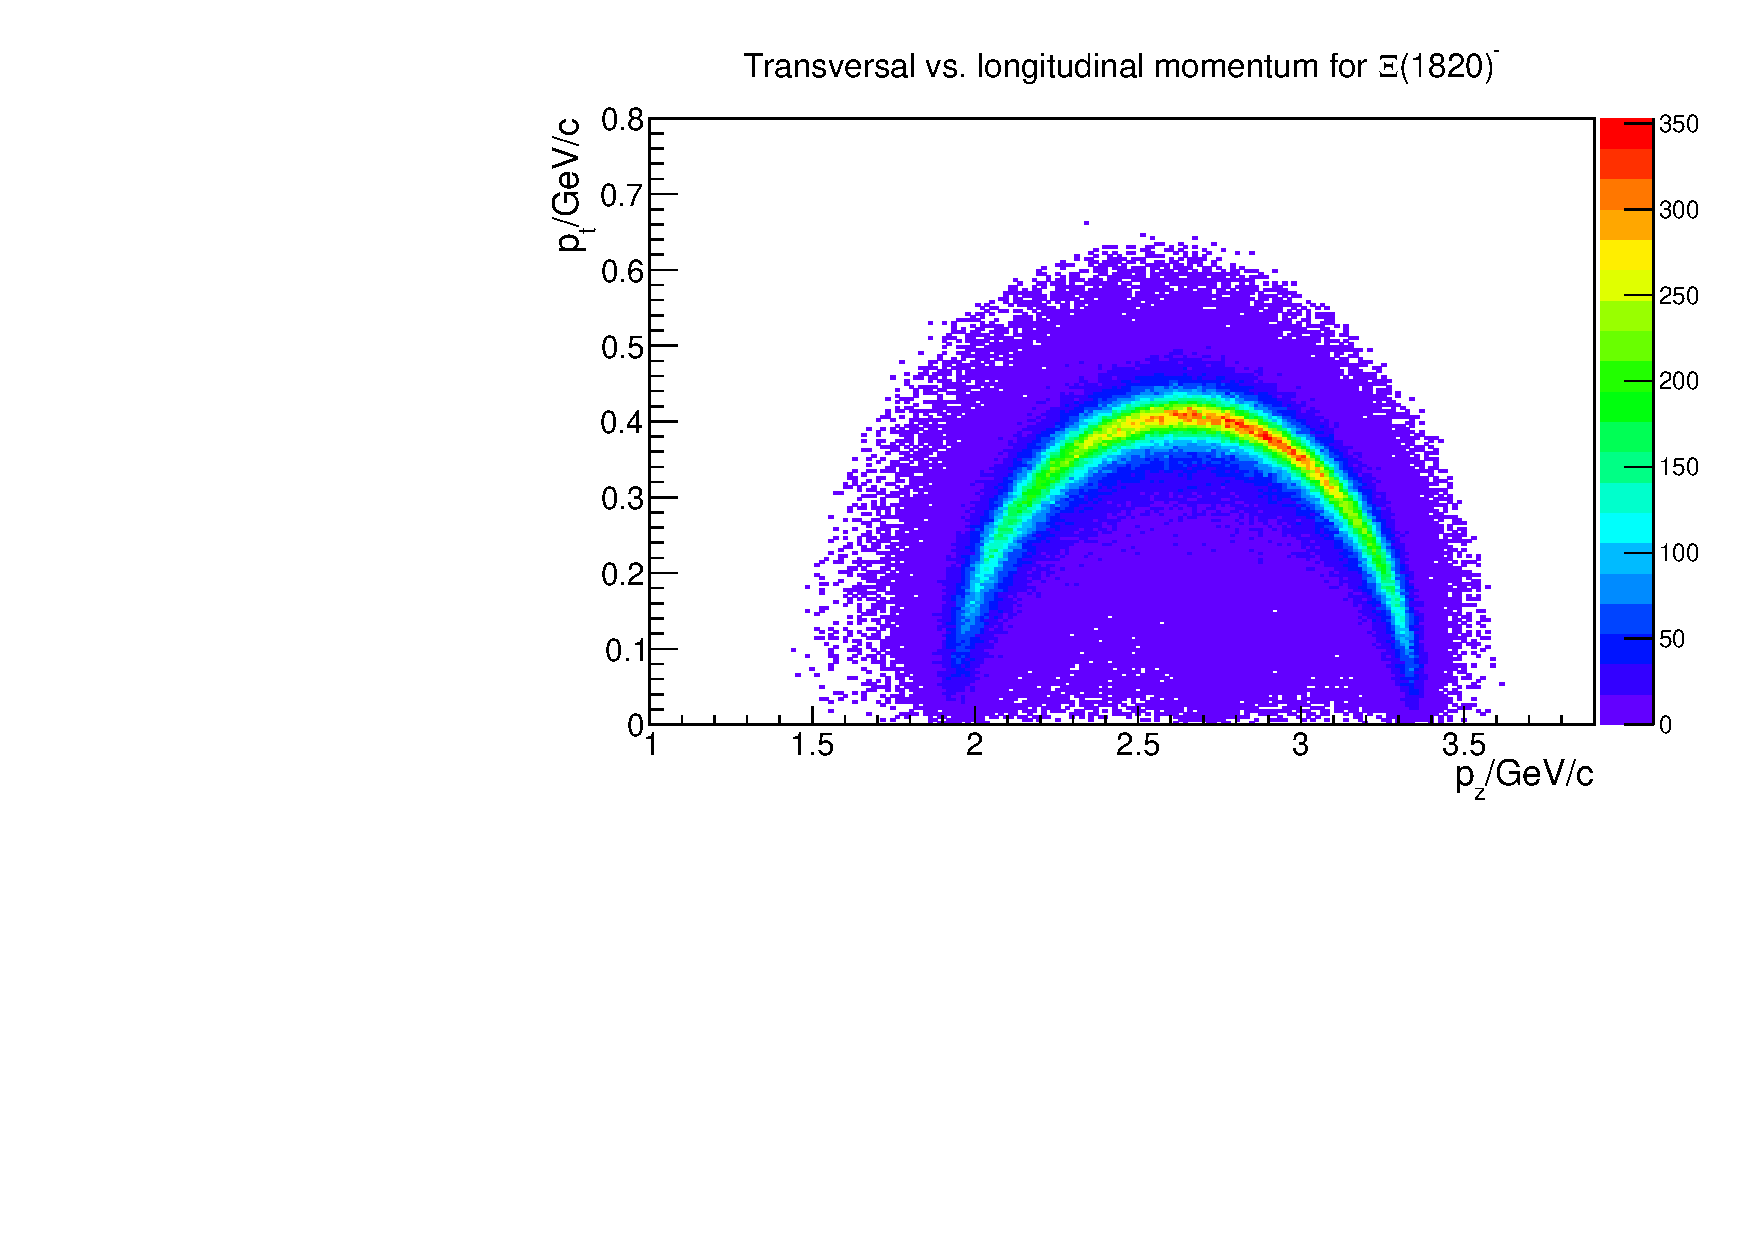
\includegraphics[width=0.49\textwidth]{./plots/Xi1820/XiMinus1820_pt_vs_pz_cut.pdf}}
		\subfigure[\excitedanticascade]{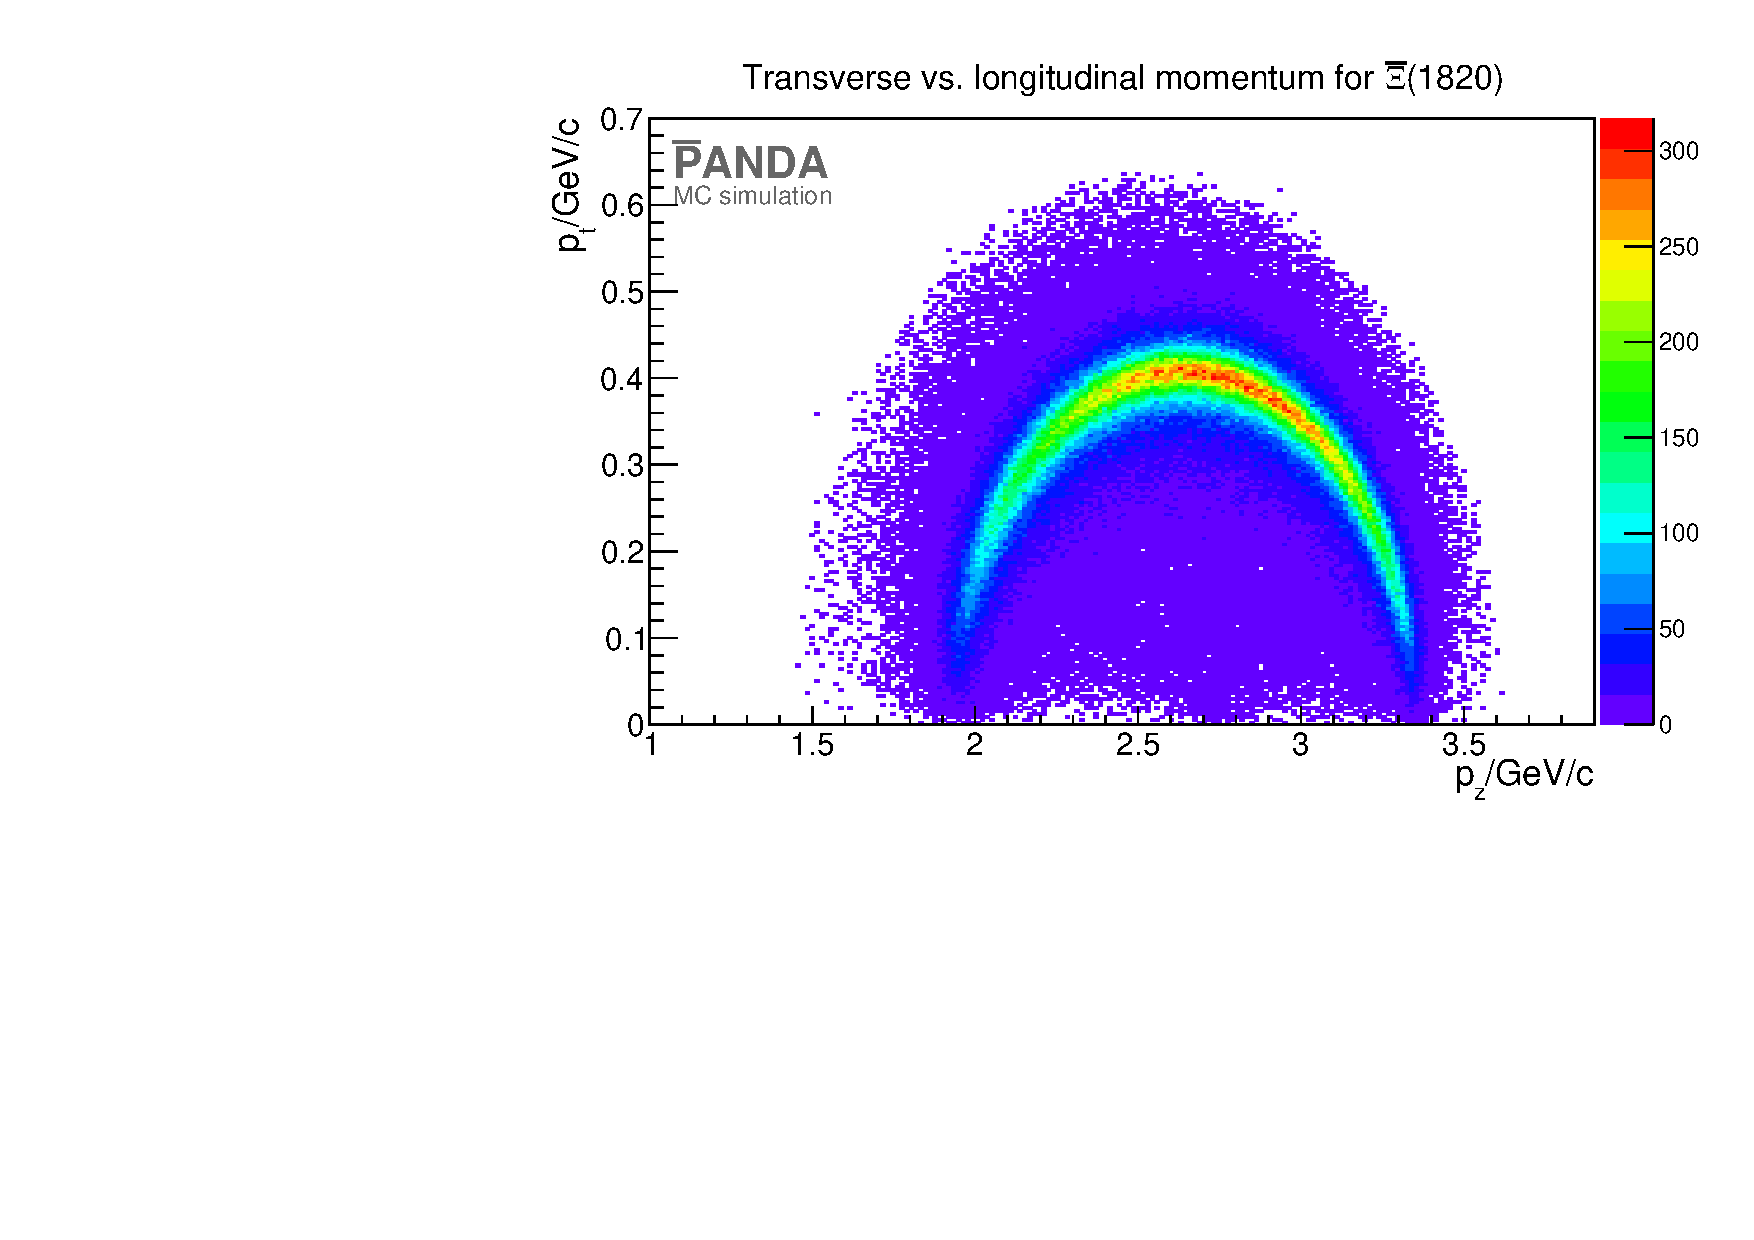
\includegraphics[width=0.49\textwidth]{./plots/Xi1820/XiPlus1820_pt_vs_pz_cut.pdf}}
		\caption{\propose Both plots show the longitudinal versus the transverse momentum of the excited cascade baryon.}
		\label{fig:xi1820_pt_vs_pz}
	\end{figure}
	
	The reconstructed distributions are in good agreement with the distribution coming from the simulated events which are 
	shown in figure \ref{fig:MC_xi_pt_vs_pz} (b).
	
\section{Reconstruction of the whole reaction chain}

	\subsection*{Selection}
	
	To reconstruct the whole reaction chain \excitedcascade and \anticascade are combined.
	This is also done with \excitedanticascade and \cascade for the charge conjugated channel.
	For this reconstruction the event selection is done with an exclusive method.
	The resulting four-momentum vector of both daughter particles --  here \excitedcascade 
	and \anticascade and there charge conjugate. particles -- is fitted with the constraint to match to the initial for momentum vector  

	\begin{center}
		\begin{equation}\nonumber
			\left(\mt{p}_x,\, \mt{p}_y,\, \mt{p}_z,\, \mt{E} \right) = \left(0,\, 0,\, 4.6,\, 5.63 \right)
		\end{equation}
	\end{center}
	of the \pbarpSystem.	
	This fit is performed with the PndKinFitter.
	After the four-momentum fit only those candidates are selected which have a \chisq probability of more than $1\%$.
	The \chisq probability is shown in figure \ref{fig:xisys_prob}. 
	The red line denotes the cut value.

	\begin{figure}
		\centering
		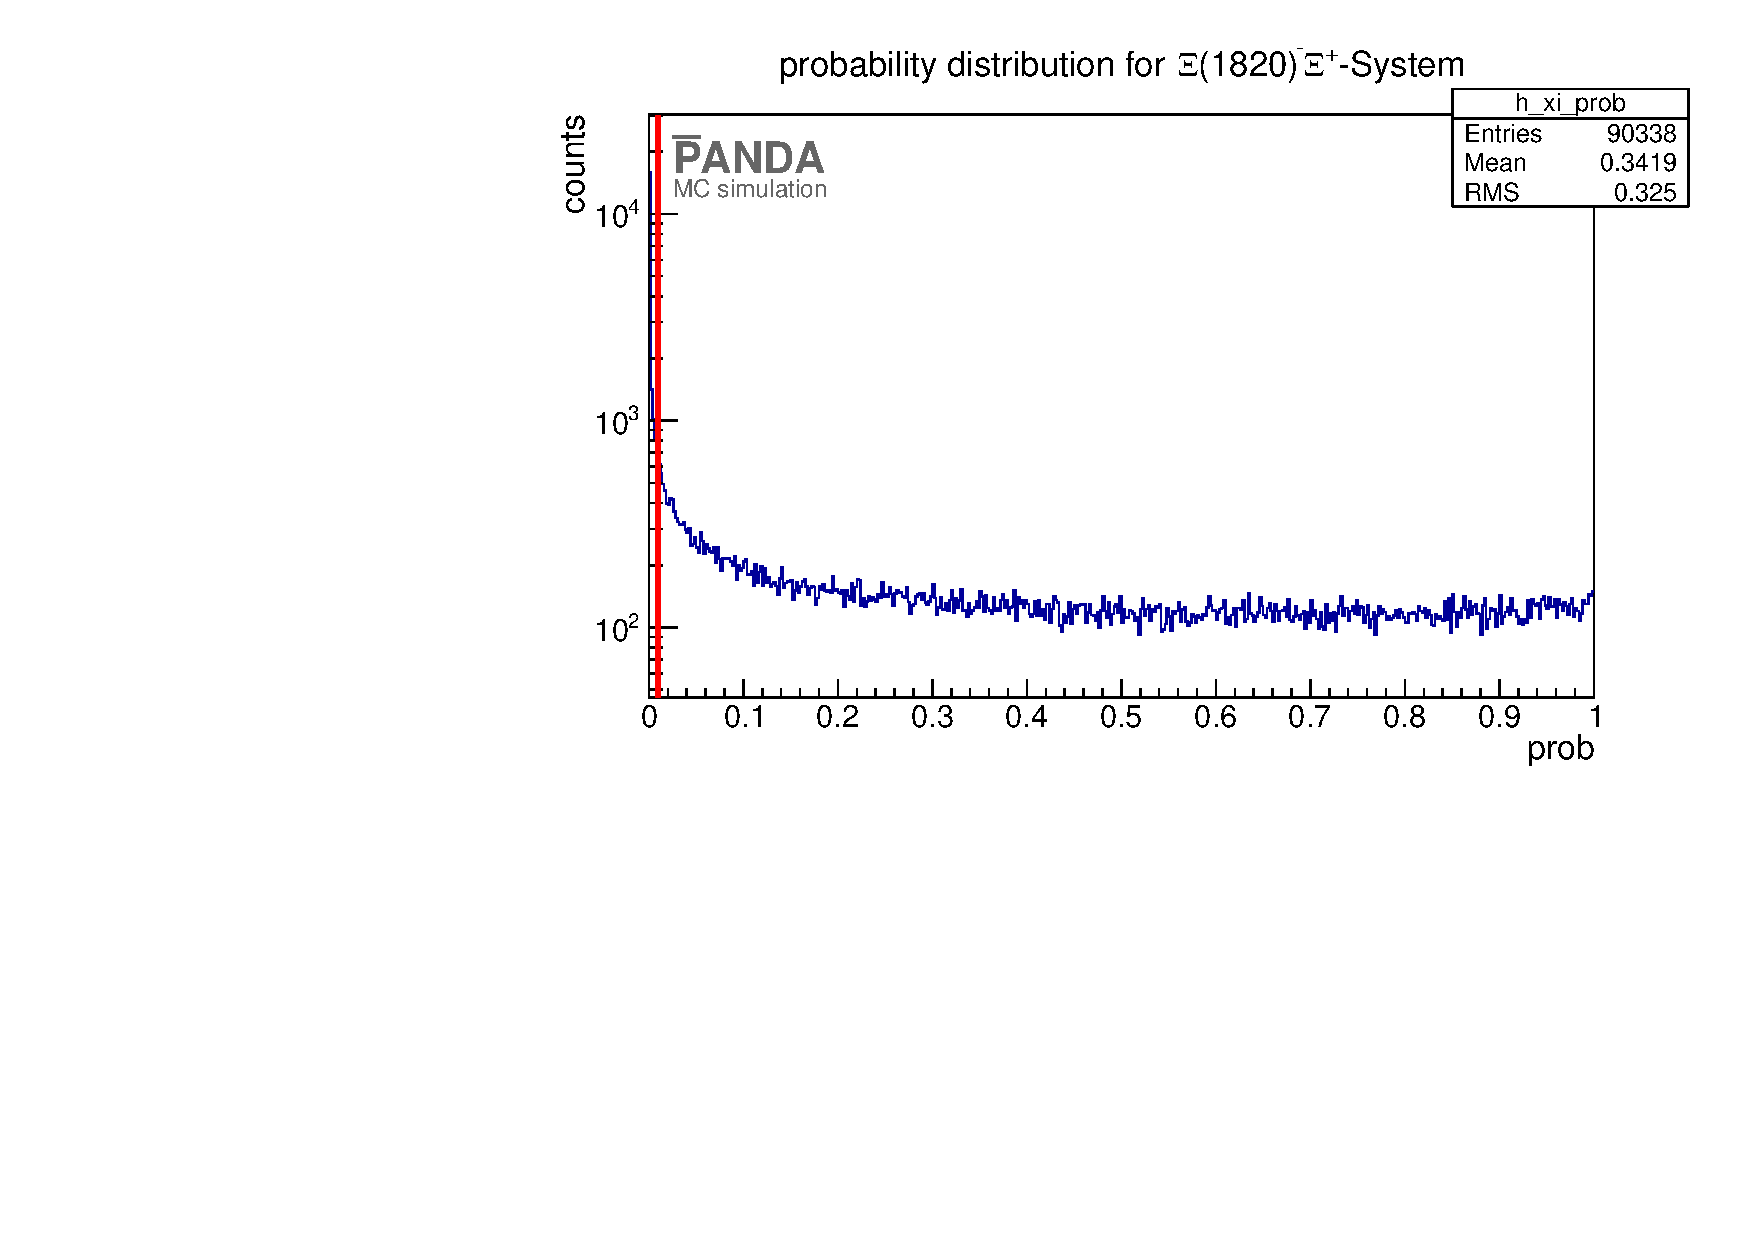
\includegraphics[width=0.7\textwidth]{./plots/pbarp/XiSys_prob.pdf}
		\caption{\propose 4-constraint fit probability. The red line denotes the cut value of $1\%$.}
		\label{fig:xisys_prob}
	\end{figure}
	
	The selection scheme is shown in figure \ref{fig:fourconstraintfit}
	 
	\begin{figure}
		\centering
			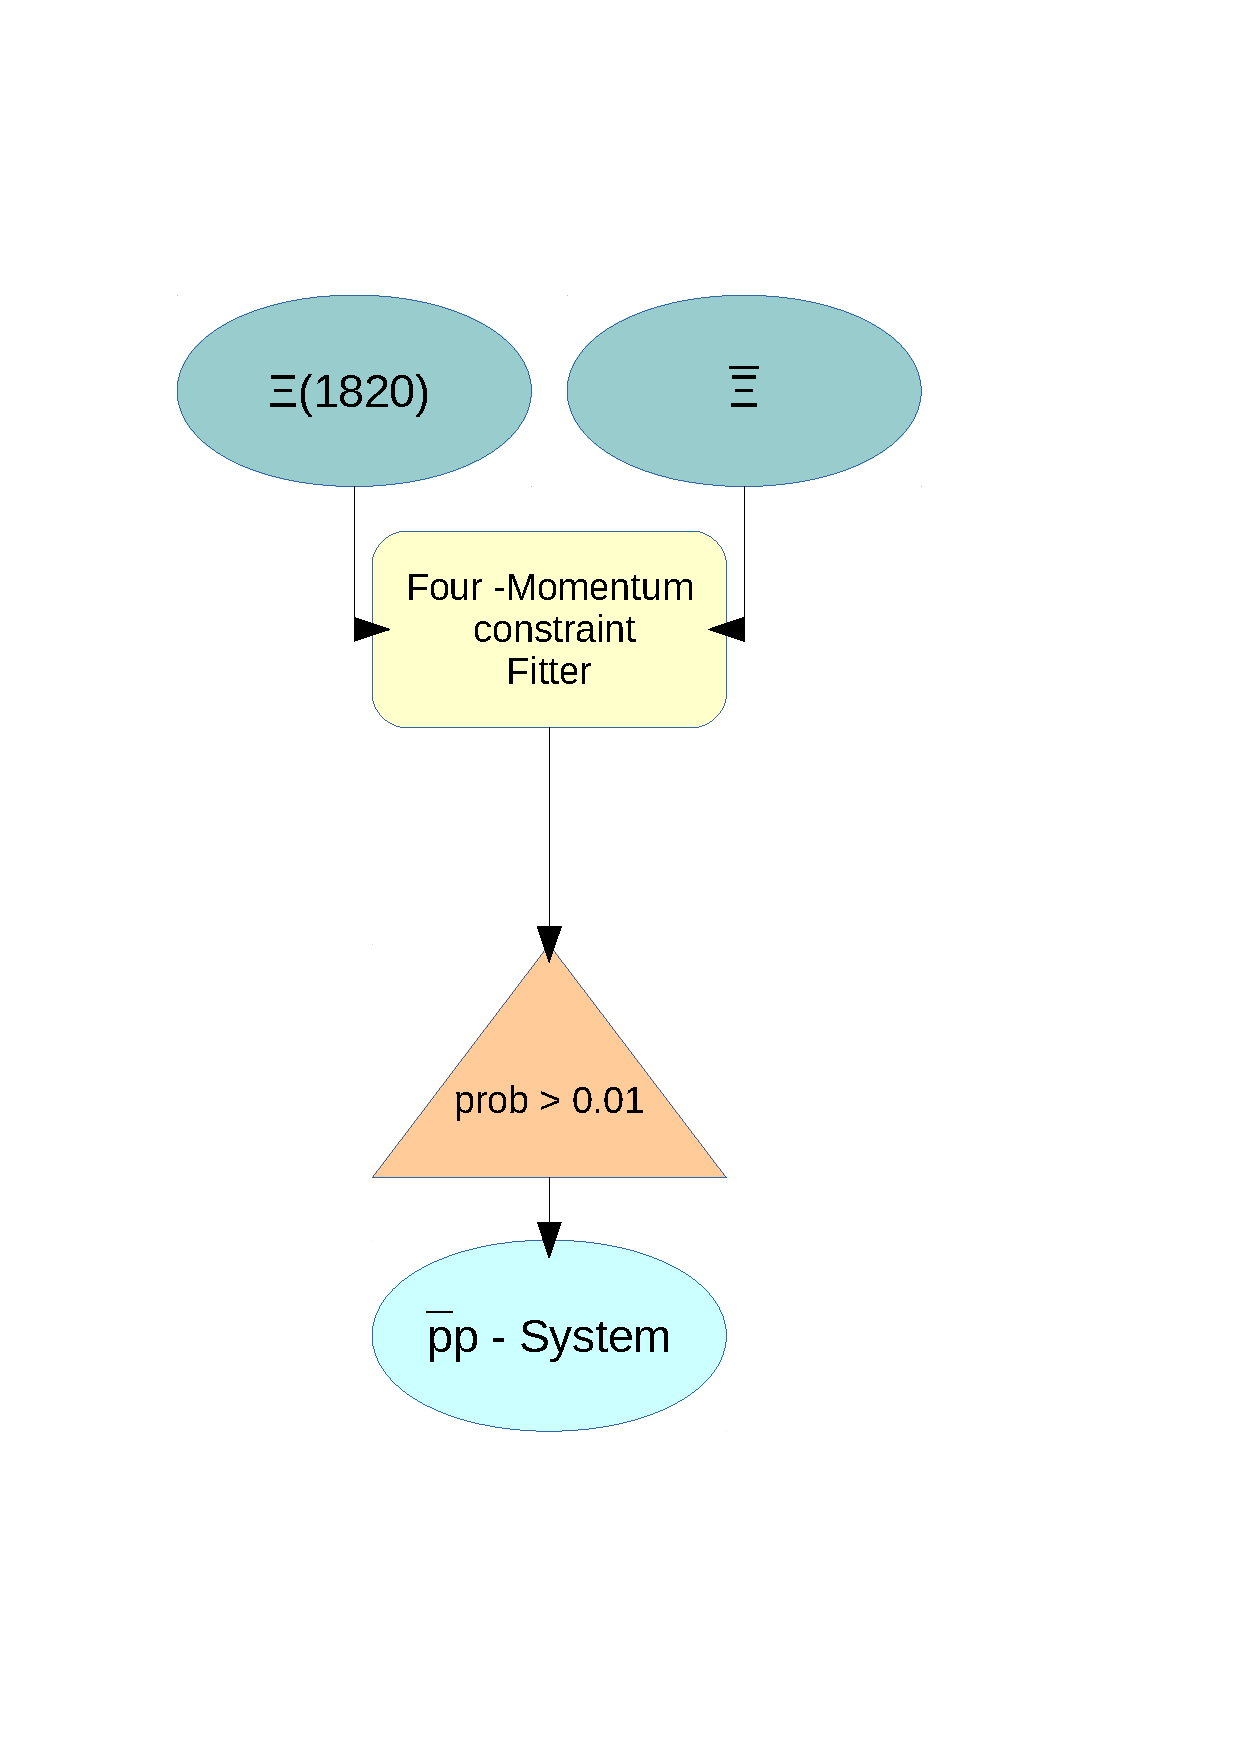
\includegraphics[width=0.50\textwidth]{./plots/combineCascadeSys.pdf}
		\caption{\propose Scheme for the reconstruction of the whole reaction chain.}
		\label{fig:fourconstraintfit}
	\end{figure}
	
	\subsection*{Results}
	
	The results of the reconstruction efficiency for all non-final state particles is shown in table \ref{tab:non-finalstate_efficiency}
	and table \ref{tab:non-finalstate_efficiency_cc}.
	
	\begin{table}
		\centering
		\caption{\propose reconstruction efficiency for non-final state particles for \pbarpSystem $\rightarrow$ \excitedcascade \anticascade}
		\label{tab:non-finalstate_efficiency}
		
		\begin{tabular}{lcc}
		
			\hline
			particle & reco. efficiency in $\%$ & dp/p in $\%$ \\\hline
			\hline
			\lam & 50.33&   1.50 \\
			\alam & 41.46&   1.45\\
			\anticascade & 18.39&   1.29\\
			\excitedcascade & 32.02&   2.68 \\
			\excitedcascade \anticascade system & 4.69&   1.03\\\hline
			 	
		\end{tabular}
	\end{table}
	
		\begin{table}
		\centering
		\caption{\propose reconstruction efficiency for non-final state particles for \pbarpSystem $\rightarrow$ \excitedanticascade \cascade}
		\label{tab:non-finalstate_efficiency_cc}
		
		\begin{tabular}{lcc}
		
			\hline
			particle & reco. efficiency in $\%$ & dp/p in $\%$ \\\hline
			\hline
			\lam & 42.47&   1.45 \\
			\alam & 49.0&   1.50\\
			\cascade & 18.64&   2.30\\
			\excitedanticascade & 33.22&   1.31\\
			\excitedanticascade \cascade system & 4.87&   1.03\\\hline
			 	
		\end{tabular}
	\end{table}
	
	Figure \ref{fig:reco_Dalitzplot} shows the Dalitz plot for the \anticascade, \lam and \kminus final states after the reconstruction. 
	Compared with the Dalitz plot of the simulated particles shown in figure \ref{fig:eventgeneration_Dalitz} the reconstruction seems to be good.
	
	\begin{figure}
		\centering
		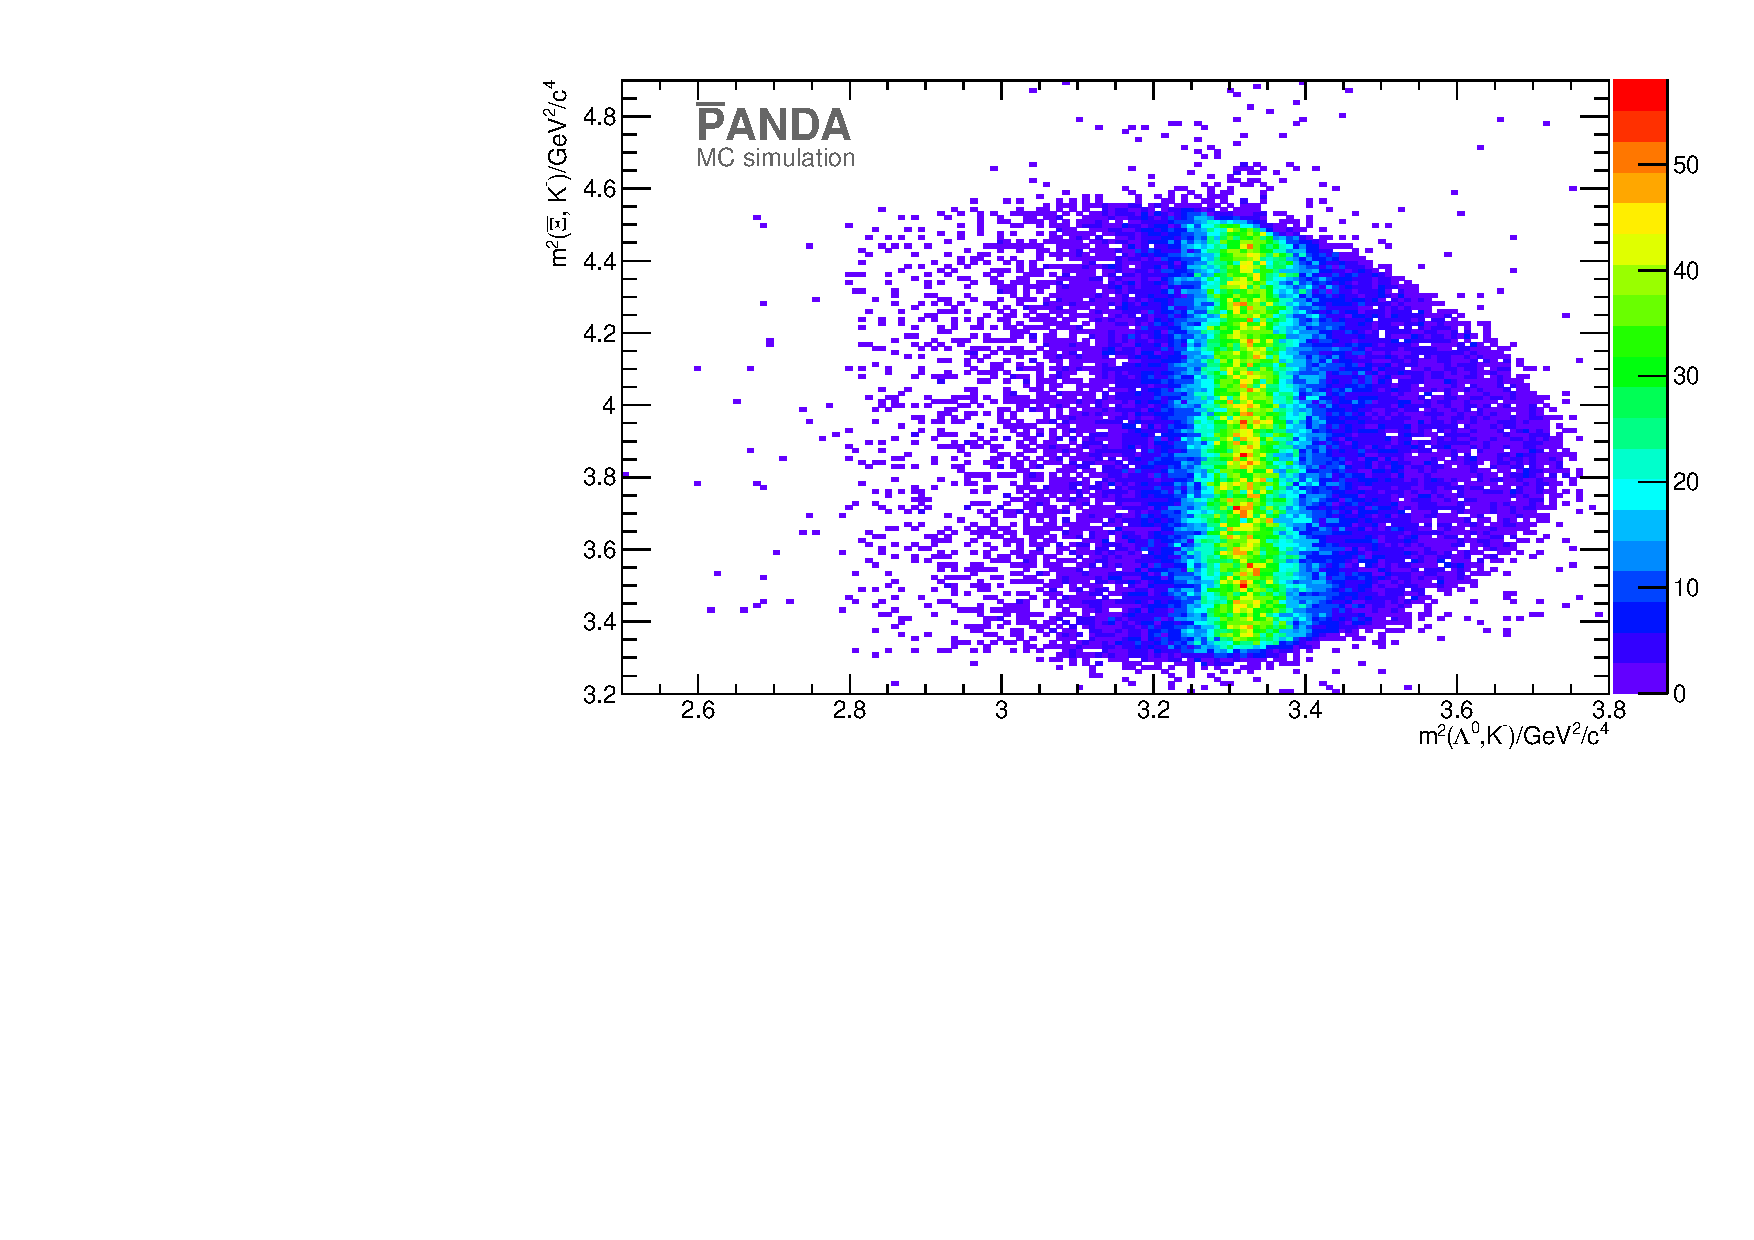
\includegraphics[width=0.8\textwidth]{./plots/pbarp/Dalitzplot_reco.pdf}
		\caption{\propose Dalitz plot for reconstructed particles}
		\label{fig:reco_Dalitzplot}
	
	\end{figure}
	
	